\documentclass[a4paper,12pt,twoside]{memoir}
\usepackage[trainermanual]{btp}    % Use the trainermanual package option (i.e. \usepackage[trainermanual]{btp}) to generate the Trainer's version of the manual
%\usepackage[
%  noinfo,
%  cam,
%  cross,                % crosses as marks
%  a4,
%  width=6.25in,         % the width of the galley
%  height=9.25in,        % the height of the galley
%  center                % actual page is centered on the galley
%]{crop}
% Set some Workshop specific info
\setWorkshopTitle{Introduction to Next Generation Sequencing Hands-on Workshop}
\setWorkshopVenue{}
\setWorkshopDate{}
\setWorkshopAuthor{
Bioplatforms Australia (BPA)\\
The Commonwealth Scientific and Industrial Research Organisation (CSIRO)\\
}

\begin{document}

%
% Workshop Title Page
%
\workshoptitlepage

%
% CC-BY
%
\chapter{Licensing}

This work is licensed under a Creative Commons Attribution 3.0 Unported License and
the below text is a summary of the main terms of the full Legal Code (the full licence) available at
\url{http://creativecommons.org/licenses/by/3.0/legalcode}.

\begin{description}[style=multiline,labelindent=0cm,align=left,leftmargin=1.5cm]
\item[You are free:] \hfill

to copy, distribute, display, and perform the work 

to make derivative works

to make commercial use of the work
  
\item[Under the following conditions:] \hfill

  \textbf{Attribution} - You must give the original author credit.
  
\item[With the understanding that:] \hfill

  \textbf{Waiver} - Any of the above conditions can be waived if you get permission from the
  copyright holder.
  
  \textbf{Public Domain} - Where the work or any of its elements is in the public domain
  under applicable law, that status is in no way affected by the license.
  
  \textbf{Other Rights} - In no way are any of the following rights affected by the license:
  
  \begin{itemize}
    \item Your fair dealing or fair use rights, or other applicable copyright exceptions and limitations;
  
    \item The author's moral rights;
  
    \item Rights other persons may have either in the work itself or in how the work is used, such
    as publicity or privacy rights.
  \end{itemize}
  
  \textbf{Notice} - For any reuse or distribution, you must make clear to others the
  licence terms of this work.
  
\end{description}

\vspace{\fill}

\begin{center}

\includegraphics[height=1cm]{./licences/cc_by.png}
\end{center}

\clearpage

\tableofcontents

\chapter{Workshop Information}
\clearpage

%
% Trainers Page
%
\section{The Trainers}

\newlength{\trainerIconWidth}
\setlength{\trainerIconWidth}{2.0cm}

\begin{table}[H]
  \centering
  \small
  \renewcommand{\arraystretch}{1}
  %\caption{A table arranging  images}
  \rowcolors{1}{gray!25}{white}
  \begin{tabular}{>{\centering\arraybackslash} m{1.1\trainerIconWidth} m{1\textwidth}}
    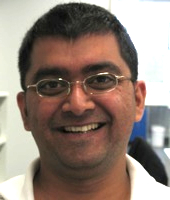
\includegraphics[width=\trainerIconWidth]{trainers/Deshpande.jpg} & 
      \textbf{Dr. Nandan Deshpande}\newline
      
      Research Associate\newline
      The University of New South Wales (UNSW), NSW\newline
      \mailto{n.deshpande@unsw.edu.au}\\
    
    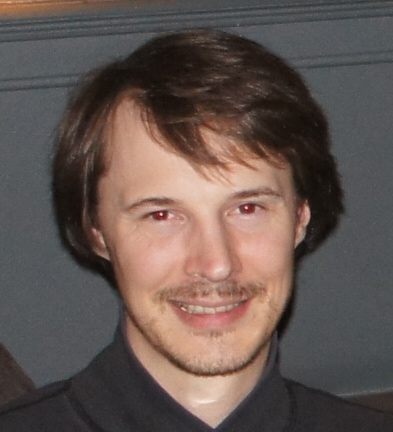
\includegraphics[width=\trainerIconWidth]{trainers/Duesing.jpg} & 
      \textbf{Dr. Konsta Duesing}\newline
      
      Research Team Leader - Statistics \& Bioinformatics\newline
      CSIRO Animal, Food and Health Science, NSW\newline
      \mailto{konsta.duesing@csiro.au}\\
    
    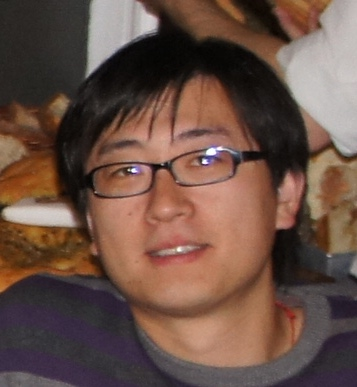
\includegraphics[width=\trainerIconWidth]{trainers/Li.jpg} & 
      \textbf{Dr. Xi (Sean) Li}\newline
      
      Bioinformatics Analyst\newline
      Bioinformatics Core, CSIRO Mathematics, Informatics and Statistics, ACT\newline
      \mailto{sean.li@csiro.au}\\
    
    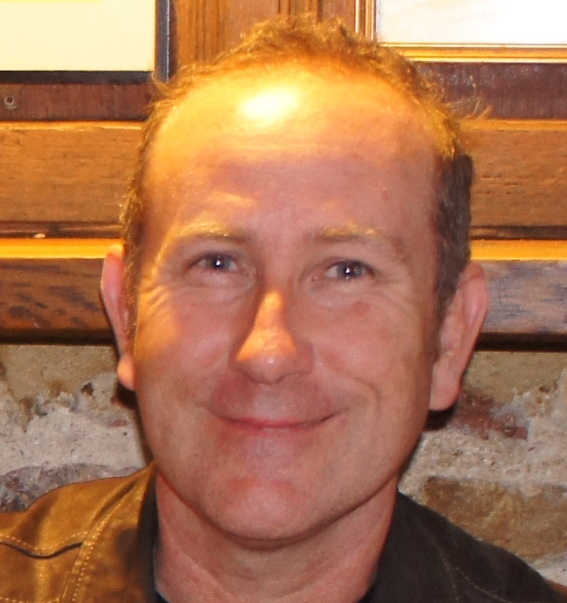
\includegraphics[width=\trainerIconWidth]{trainers/McWilliam.jpg} & 
      \textbf{Mr. Sean McWilliam}\newline
      
      Bioinformatics Analyst\newline
      CSIRO Animal, Food and Health Sciences, QLD\newline
      \mailto{sean.mcwilliam@csiro.au}\\
    
    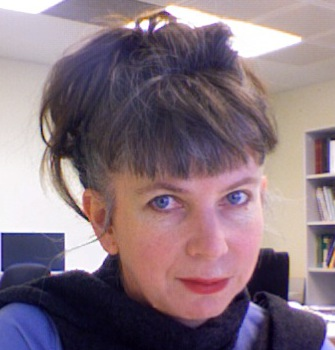
\includegraphics[width=\trainerIconWidth]{trainers/Moolhuijzen.jpg} & 
      \textbf{Dr. Paula Moolhuijzen}\newline
      
      Senior Bioinformatics Officer\newline
      Centre for Comparative Genomics, Murdoch University, WA\newline
      \mailto{pmoolhuijzen@ccg.murdoch.edu.au}\\
    
    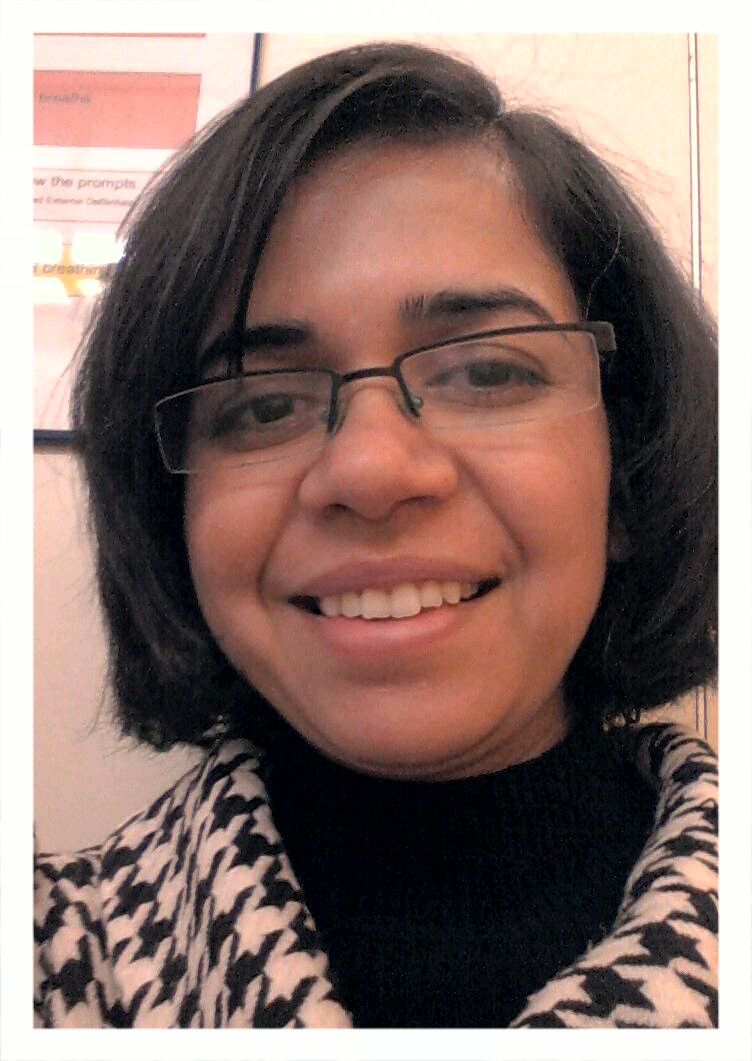
\includegraphics[width=\trainerIconWidth]{trainers/Tyagi.jpg} & 
      \textbf{Dr. Sonika Tyagi}\newline
      
      Bioinformatics Supervisor\newline
      Australian Genome Research Facility Ltd, The Walter and Eliza Hall Institute, VIC\newline
      \mailto{sonika.tyagi@agrf.org.au}\\
    
    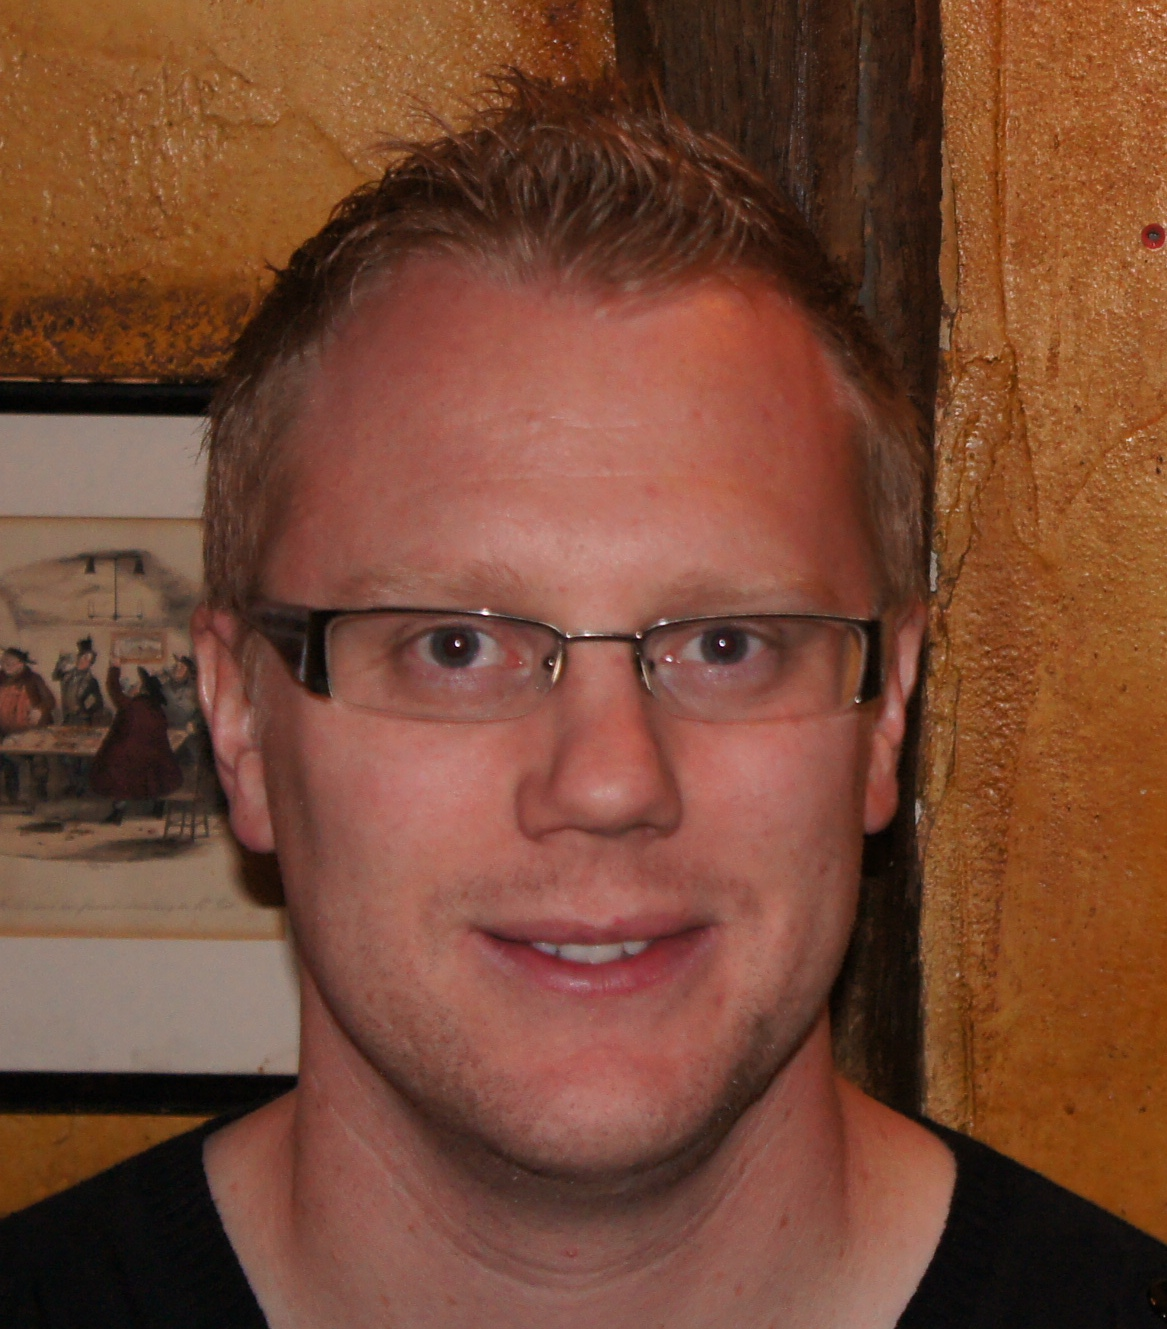
\includegraphics[width=\trainerIconWidth]{trainers/watson-haigh.jpeg} & 
      \textbf{Dr. Nathan S. Watson-Haigh}\newline
      
      Research Fellow in Bioinformatics\newline
      The Australian Centre for Plant Functional Genomics (ACPFG), SA\newline
      \mailto{nathan.haigh@acpfg.com.au}\\
    
    \end{tabular}
  \caption{\label{tab:trainers}}
\end{table}


%
% Workshop Preamble
%
%
% Start: General Information describing the workshop and the structure of the handouts
%
\newpage

% \section{Do's and Don'ts of the Workshop}
% TODO Add do's and don'ts e.g. email, social media etc 

\section{Providing Feedback}
While we endeavour to deliver a workshop with quality content and documentation
in a venue conducive to an exciting, well run hands-on workshop with a bunch of
knowledgeable and likable trainers, we know there are things we could do better.

Whilst we want to know what didn't quite hit the mark for you, what would be
most helpful and least depressing, would be for you to provide ways to improve
the workshop. i.e. constructive feedback. After all, if we knew something wasn't
going to work, we wouldn't have done it or put it into the workshop in the first
place! Remember, we're experts in the field of bioinformatics not experts in the
field of biology!

Clearly, we also want to know what we did well! This gives us that ``feel good''
factor which will see us through those long days and nights in the lead up to
such hands-on workshops!

With that in mind, we'll provide three really high tech mechanism through which you
can provide anonymous feedback during the workshop:
\begin{enumerate}
  \item A sheet of paper, from a flip-chart, sporting a ``happy'' face and a
  ``not so happy'' face. Armed with a stack of colourful post-it notes, your
  mission is to see how many comments you can stick on the ``happy'' side!
  
  \item Some empty ruled pages at the back of this handout. Use them for your
  own personal notes or for write specific comments/feedback about the workshop
  as it progresses.
  
  \item An online post-workshop evaluation survey. We'll ask you to complete
  this before you leave. If you've used the blank pages at the back of this
  handout to make feedback notes, you'll be able to provide more specific and
  helpful feedback with the least amount of brain-drain!
\end{enumerate}

\section{Document Structure}
We have provided you with an electronic copy of the workshop's hands-on tutorial documents.
We have done this for two reasons: 1) you will have something to take away with you at the 
end of the workshop, and 2) you can save time (mis)typing commands on the command line by using
copy-and-paste.

\emph{We advise you to use Acrobat Reader to view the PDF. This is because it
properly supports some features we have implemented to ensure that
copy-and-paste of commands works as expected. This includes the appropriate
copy-and-paste of special characters like tilde and hyphens as well as skipping
line numbers for easy copy-and-past of whole code blocks.}

\begin{warning}
While you could fly through the hands-on sessions doing
copy-and-paste you will learn more if you take the time, saved from not having to type all those
commands, to understand what each command is doing!
\end{warning}

The commands to enter at a terminal look something like this:
\begin{lstlisting}
tophat --solexa-quals -g 2 --library-type fr-unstranded -j annotation/Danio_rerio.Zv9.66.spliceSites -o tophat/ZV9_2cells genome/ZV9 data/2cells_1.fastq data/2cells_2.fastq
\end{lstlisting}  

The following styled code is not to be entered at a terminal, it is simply to
show you the syntax of the command. You must use your own judgement to
substitute in the correct arguments, options, filenames etc

\begin{lstlisting}[style=command_syntax]
tophat [options]* <index_base> <reads_1> <reads_2>
\end{lstlisting}

The following is an example how of R commands are styled:

\begin{lstlisting}[style=R]
R --no-save
library(plotrix) 
data <- read.table("run_25/stats.txt", header=TRUE) 
weighted.hist(data$short1_cov+data$short2_cov, data$lgth, breaks=0:70)
q()
\end{lstlisting}

The following icons are used in the margin, throughout the documentation to help
you navigate around the document more easily:

% TODO limit the use of some icons throughout as some are clearly overused and confuse the eye
\hspace*{.2cm}\vcent{
\includegraphics[height=1cm]{./icons/info.png}} Important\\
\hspace*{.2cm}\vcent{
\includegraphics[height=1cm]{./icons/notes.png}} For reference\\
\hspace*{.2cm}\vcent{
\includegraphics[height=1cm]{./icons/steps.png}} Follow these steps\\
\hspace*{.2cm}\vcent{
\includegraphics[height=1cm]{./icons/questions.png}} Questions to answer\\
\hspace*{.2cm}\vcent{
\includegraphics[height=1cm]{./icons/warning.png}} Warning - STOP and read\\
\hspace*{.2cm}\vcent{
\includegraphics[height=1cm]{./icons/bonus1.png}} Bonus exercise for fast learners\\
\hspace*{.2cm}\vcent{
\includegraphics[height=1cm]{./icons/bonus2.png}} Advanced exercise for super-fast learners\\

\section{Resources Used}
We have provided you with an environment which contains all the tools and data
you need for the duration of this workshop. However, we also provide details
about the tools and data used by each module at the start of the respective
module documentation.


%
% Start of modules
% Switch chapter styling to module
%
\chapterstyle{module}

%
% QC Module
%
% Define the top matter
\setModuleTitle{Data Quality}
\setModuleAuthors{%
  Sonika Tyagi \mailto{sonika.tyagi@agrf.org.au}
}
\setModuleContributions{%
  Nathan S. Watson-Haigh \mailto{nathan.watson-haigh@awri.com.au}%
}

% Start: Module Title Page
\chapter{\moduleTitle}
\newpage
% End: Module Title Page

\section{Key Learning Outcomes}

After completing this practical the trainee should be able to:
\begin{itemize}
  \item Assess the overall quality of NGS sequence reads
  \item Visualise the quality, and other associated matrices, of reads to decide
        on filters and cutoffs for cleaning up data ready for downstream analysis
  \item Clean up and pre-process the sequences data for further analysis
\end{itemize}

\section{Resources You'll be Using}
 
\subsection{Tools Used}
\begin{description}[style=multiline,labelindent=0cm,align=left,leftmargin=0.5cm]
  \item[FastQC]\hfill\\
  	\url{http://www.bioinformatics.babraham.ac.uk/projects/fastqc/}
  \item[FASTX-Toolkit]\hfill\\
  	\url{http://hannonlab.cshl.edu/fastx_toolkit/}
  \item[Picard]\hfill\\
  	\url{http://picard.sourceforge.net/}
\end{description}

\section{Useful Links}
 
\begin{description}[style=multiline,labelindent=0cm,align=left,leftmargin=0.5cm]
  \item[FASTQ Encoding]\hfill\\
    \url{http://en.wikipedia.org/wiki/FASTQ_format#Encoding}
\end{description}

% \subsection{Sources of Data}
% TODO Provide a publically available data set used for this module
% \url{http://www.ebi.ac.uk/ena/data/view/ERR022484}\\
% \url{http://www.ebi.ac.uk/ena/data/view/ERR022485}

\newpage

\section{Introduction}

\begin{note}
Going on a blind date with your read set? For a better understanding of the
consequences please check the data quality!
\end{note}

For the purpose of this tutorial we are focusing only on Illumina sequencing
which uses 'sequence by synthesis' technology in a highly parallel fashion.
Although Illumina high throughput  sequencing provides highly accurate sequence
data, several sequence artifacts, including base calling errors and small
insertions/deletions, poor quality reads and primer/adapter contamination are
quite common in the high throughput sequencing data. The primary errors are
substitution errors. The error rates can vary from 0.5-2.0\% with errors mainly
rising in frequency at the 3' ends of reads.

One way to investigate sequence data quality is to visualize the quality scores
and other metrics in a compact manner to get an idea about the quality of a read
data set. Read data sets can be improved by post processing in different ways
like trimming off low quality bases, cleaning up any sequencing adapters and
removing PCR duplicates. We can also look at other statistics such
as, sequence length distribution, base composition, sequence complexity,
presence of ambiguous bases etc. to assess the overall quality of the data set.

Highly redundant coverage ($>$15X) of the genome can be used to correct sequencing
errors in the reads before assembly and errors. Various k-mer based error
correction methods exist but are beyond the scope of this tutorial.

\subsection{Quality Value Encoding Schema}

In order to use a single character to encode Phred qualities, ASCII characters
are used (\url{http://shop.alterlinks.com/ascii-table/ascii-table-us.php}). All ASCII characters have a decimal
number associated with them but the first 32 characters are non-printable (e.g.
backspace, shift, return, escape). Therefore, the first printable ASCII
character is number 33, the exclamation mark (!). In Phred+33 encoded quality
values the exclamation mark takes the Phred quality score of zero.

Early Solexa (now Illumina) sequencing needed to encode negative quality values.
Because ASCII characters $<$ 33 are non-printable, using the Phred+33 encoding was
not possible. Therefore, they simply moved the offset from 33 to 64 thus
inventing the Phred+64 encoded quality values. In this encoding a Phred quality
of zero is denoted by the ASCII number 64 (the @ character). Since Illumina 1.8,
quality values are now encoded using Phred+33.

FASTQ does not provide a way to describe what quality encoding is used for the
quality values. Therefore, you should find this out from your sequencing
provider. Alternatively, you may be able to figure this out by determining what
ASCII characters are present in the FASTQ file. E.g the presence of numbers in
the quality strings, can only mean the quality values are Phred+33 encoded.
However, due to the overlapping nature of the Phred+33 and Phred+64 encoding
schema it is not always possible to identify what encoding is in use. For
example, if the only characters seen in the quality string are (\texttt{@ABCDEFGHI}),
then it is impossible to know if you have really good Phred+33 encoded qualities
or really bad Phred+64 encoded qualities.

For a grapical representation of the different ASCII characters used in the two
encoding schema see: \url{http://en.wikipedia.org/wiki/FASTQ_format#Encoding}.

\section{Prepare the Environment}

\begin{information}
To investigate sequence data quality we will demonstrate tools called FastQC
and FASTX-Toolkit. FastQC will process and present the reports in a visual manner.
Based on the results, the sequence data can be processed using the FASTX-Toolkit.
We will use one data set in this practical, which can be found in the QC
directory on your desktop.
\end{information}

\begin{steps}
Open the Terminal and go to the directory where the data are stored:
\begin{lstlisting}
cd ~/QC/
pwd
\end{lstlisting}

At any time, help can be displayed for FastQC using the following command:
\begin{lstlisting}
fastqc -h
\end{lstlisting}

\end{steps}


\section{Quality Visualisation}

\begin{information}
We have a file for a good quality and bad quality statistics. FastQC generates
results in the form of a zipped and unzipped directory for each input file.
\end{information}

\begin{steps}
Execute the following command on the two files:
\begin{lstlisting}
fastqc -f fastq bad_example.fastq 
fastqc -f fastq good_example.fastq
\end{lstlisting}

View the FastQC report file of the bad data using a web browser such as
firefox.

\begin{lstlisting}
firefox bad_example_fastqc/fastqc_report.html &
\end{lstlisting}

\end{steps}

\begin{note}
The report file will have a Basic Statistics table and various graphs and tables
for different quality statistics. E.g.:
\end{note}

\begin{table}[H]
  \centering
  \caption{FastQC Basic Statistics table}
    \begin{tabular}{ll}
    \toprule
    Filename & bad\_example.fastq \\
    \midrule
    File type & Conventional base calls \\
    Encoding & Sanger / Illumina 1.9 \\
    Total Sequences & 40000 \\
    Filtered Sequences & 0 \\
    Sequence length & 100 \\
    \%GC  & 48 \\
    \bottomrule
    \end{tabular}
  \label{tab:badexampleuntrimmed}
\end{table}

\begin{figure}[H]
\centering
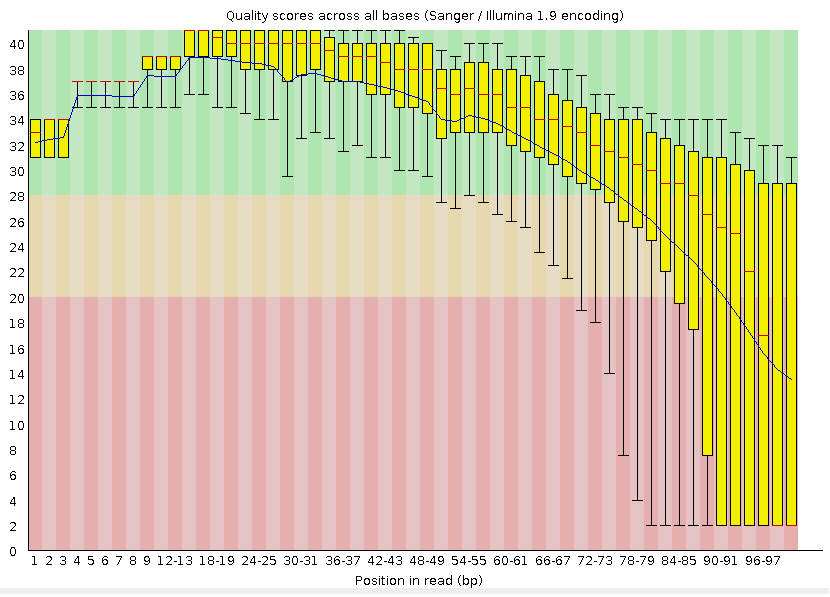
\includegraphics[width=0.8\textwidth]{ngs-qc/bad_example.png}
\caption{Per base sequence quality plot for \texttt{bad\_example.fastq}.}
\label{fig:bad_example_untrimmed_plot}
\end{figure}

\begin{information}
A Phred quality score (or Q-score) expresses an error probability.  In particular, it
serves as a convenient and compact way to communicate very small error
probabilities.
The probability that base $A$ is wrong ($P(\sim A)$) is expressed
by a quality score, $Q(A)$, according to the relationship:
\\\\
$Q(A) =-10 log10(P(\sim A))$
\\\\
The relationship between the quality score and error probability is demonstrated
with the following table:

\begin{table}[H]
  \centering
  \caption{Error probabilities associated with various quality (Q) values}
    \begin{tabular}{rrr}
    \toprule
    \textbf{Quality score, Q(A)} & \textbf{Error probability, P($\sim$A)} & \textbf{Accuracy of the base call} \\
    \midrule
    10    & 0.1     & 90\% \\
    20    & 0.01    & 99\% \\
    30    & 0.001   & 99.9\% \\
    40    & 0.0001  & 99.99\% \\
    50    & 0.00001 & 99.999\% \\
    \bottomrule
    \end{tabular}
  \label{tab:quality_error_probs}
\end{table}

\end{information}

\begin{questions}
How many sequences were there in your file? What is the read length?
\begin{answer}
40,000. read length=100bp
\end{answer}

Does the quality score values vary throughout the read length?
(hint: look at the 'per base sequence quality plot')
\begin{answer}
Yes. Quality scores are dropping towards the end of the reads.
\end{answer}

What is the quality score range you see?
\begin{answer}
2-40
\end{answer}

At around which position do the scores start falling below Q20? 
\begin{answer}
Around 80 bp position
\end{answer}


How can we trim the reads to filter out the low quality data?
\begin{answer}
By trimming off the bases after a fixed position of the read or by trimming off
bases based on the quality score.
\end{answer}
\end{questions}

\begin{bonus}
\subsection{Good Quality Data}
View the FastQC report files \texttt{fastqc\_report.html} to see examples of a good
quality data and compare the quality plot with that of the \texttt{bad\_example\_fastqc}.

\begin{lstlisting}
firefox good_example_fastqc/fastqc_report.html &
\end{lstlisting}
\end{bonus}

\begin{note}
Sequencing errors can complicate the downstream analysis, which normally
requires that reads be aligned to each other (for genome assembly) or to a
reference genome (for detection of mutations). Sequence reads containing errors
may lead to ambiguous paths in the assembly or improper gaps. In variant
analysis projects sequence reads are aligned against the reference genome. The
errors in the reads may lead to more mismatches than expected from
mutations alone. But if these errors can be removed or corrected, the read
alignments and hence the variant detection will improve. The assemblies will also
improve after pre-processing the reads with errors.
\end{note}

\section{Read Trimming}
Read trimming can be done in a variety of different ways. Choose a method
which best suits your data. Here we are giving examples of fixed-length trimming
and quality-based trimming.

\subsection{Fixed Length Trimming}
Low quality read ends can be trimmed using a fixed-length trimming. We will use the
\texttt{fastx\_trimmer} from the FASTX-Toolkit. Usage message to find out various options
you can use with this tool. Type \texttt{fastx\_trimmer -h} at anytime to display help.

\begin{steps}
We will now do fixed-length trimming of the \texttt{bad\_example.fastq} file
using the following command.
\begin{lstlisting}
cd ~/QC
fastx_trimmer -h
fastx_trimmer -Q 33 -f 1 -l 80 -i bad_example.fastq -o bad_example_trimmed01.fastq
\end{lstlisting}
\end{steps}

\begin{note}
We used the following options in the command above:
\begin{description}[style=multiline,labelindent=0cm,align=right,leftmargin=\descriptionlabelspace,rightmargin=1.5cm,font=\ttfamily]
 \item[-Q 33] Indicates the input quality scores are Phred+33 encoded
 \item[-f] First base to be retained in the output
 \item[-l] Last base to be retained in the output
 \item[-i] Input FASTQ file name
 \item[-o] Output file name
\end{description}
\end{note}

\begin{steps}
Run FastQC on the trimmed file and visualise the quality scores of the trimmed file.
\begin{lstlisting}
fastqc -f fastq bad_example_trimmed01.fastq
firefox bad_example_trimmed01_fastqc/fastqc_report.html &
\end{lstlisting}

The output should look like:

\begin{table}[H]
  \centering
  \caption{FastQC Basic Statistics table}
    \begin{tabular}{ll}
    \toprule
    Filename & bad\_example\_trimmed01.fastq\\
    \midrule
     File type & Conventional base calls\\
     Encoding & Sanger / Illumina 1.9\\
     Total Sequences & 40000\\
     Filtered Sequences & 0\\
     Sequence length & 80\\
    \%GC & 48\\
    \bottomrule
    \end{tabular}
  \label{tab:badexampletrimmed}
\end{table}

\begin{figure}[H]
\centering
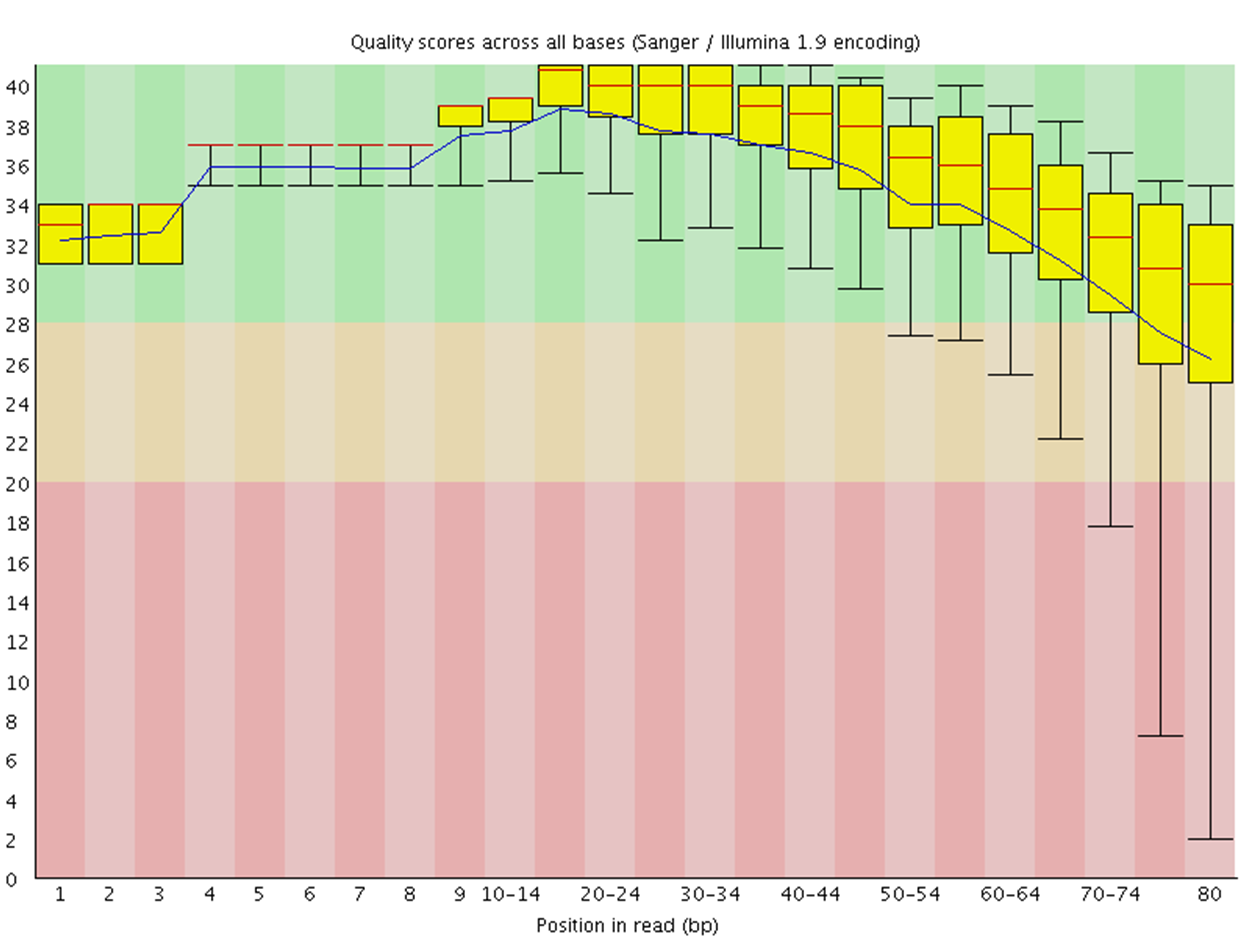
\includegraphics[width=0.8\textwidth]{ngs-qc/bad_example_trimmed_to_80bp.png}
\caption{Per base sequence quality plot for the fixed-length trimmed \texttt{bad\_example.fastq} reads.}
\label{fig:bad_example_trimmed_plot}
\end{figure}

\end{steps}

\begin{questions}
What values would you use for \texttt{-f} if you wanted to trim off 10 bases at
the 5' end of the reads?
\begin{answer}
\texttt{-f 11}
\end{answer}
\end{questions}

\subsection{Quality Based Trimming}
Base call quality scores can also be used to dynamically determine the trim
points for each read. A quality score threshold and minimum read length
following trimming can be used to remove low quality data.

\begin{steps}
Run the following command to quality trim your data:
\begin{lstlisting}
cd ~/QC
fastq_quality_trimmer -h
fastq_quality_trimmer -Q 33 -t 20 -l 50 -i bad_example.fastq -o bad_example_quality_trimmed.fastq
\end{lstlisting}
\end{steps}

\begin{note}
\begin{description}[style=multiline,labelindent=0cm,align=right,leftmargin=\descriptionlabelspace,rightmargin=1.5cm,font=\ttfamily]
 \item[-Q 33] Indicates the input quality scores are Phred+33 encoded
 \item[-t] quality score cut-off
 \item[-l] minimum length of reads to output
 \item[-i] Input FASTQ file name
 \item[-o] Output file name
\end{description}
\end{note}

\begin{steps}
Run FastQC on the quality trimmed file and visualise the quality scores.

\begin{lstlisting}
fastqc -f fastq bad_example_quality_trimmed.fastq
firefox bad_example_quality_trimmed_fastqc/fastqc_report.html &
\end{lstlisting}

The output should look like:

\begin{table}[H]
  \centering
  \caption{FastQC Basic Statistics table}
    \begin{tabular}{ll}
    \toprule
    Filename & bad\_example\_quality\_trimmed.fastq\\
    \midrule
    File type & Conventional base calls\\
    Encoding & Sanger / Illumina 1.9\\
    Total Sequences & 38976\\
    Filtered Sequences & 0\\
    Sequence length & 50-100\\
    \%GC & 48\\
    \bottomrule
    \end{tabular}
  \label{tab:badexamplequalitytrimmed}
\end{table}

\begin{figure}[H]
\centering
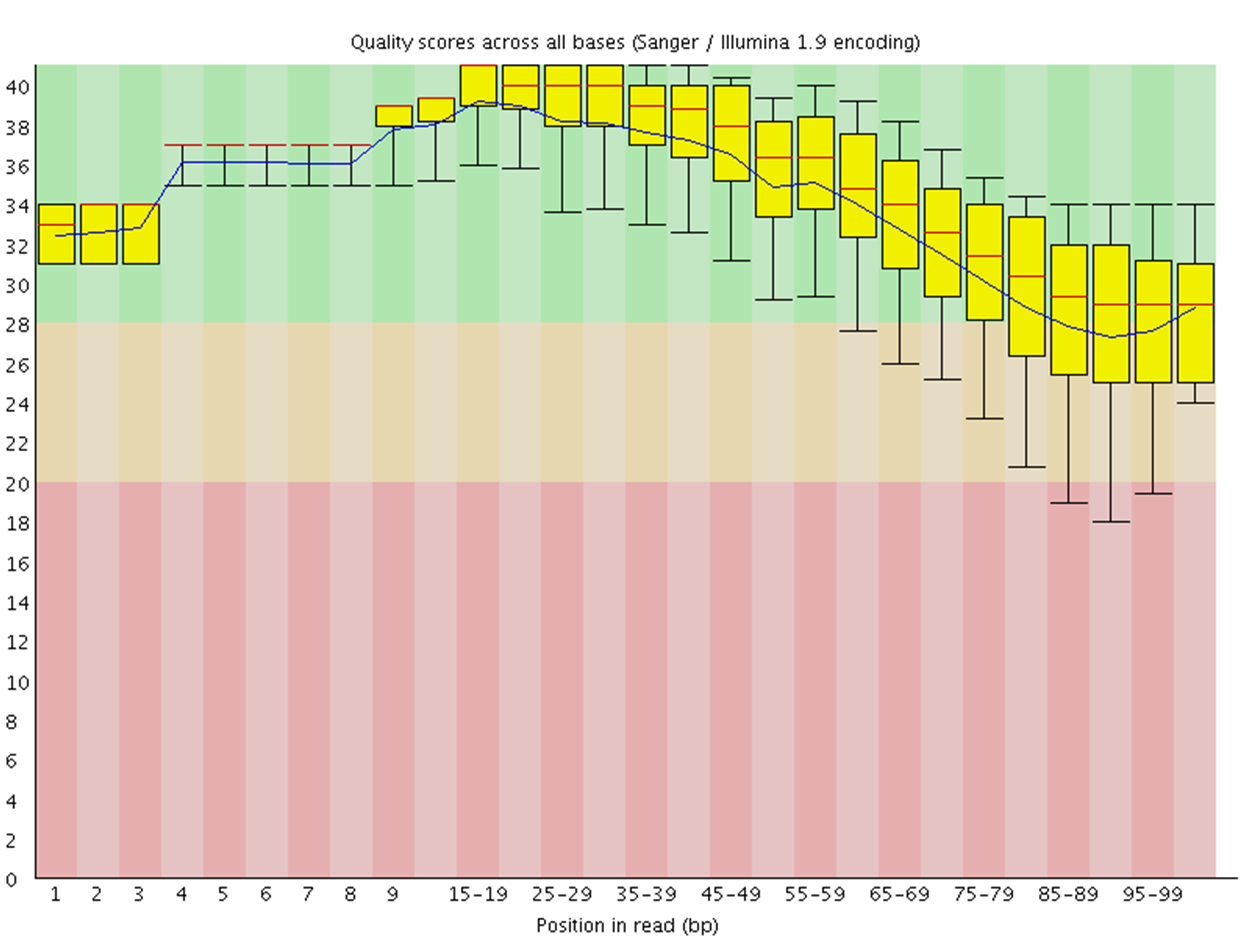
\includegraphics[width=0.8\textwidth]{ngs-qc/bad_example_quality_trimmed.png}
\caption{Per base sequence quality plot for the quality-trimmed \texttt{bad\_example.fastq} reads.}
\label{fig:bad_example_quality_trimmed_plot}
\end{figure}

\end{steps}

\begin{questions}
How did the quality score range change with two types of trimming?
\begin{answer}
Some poor quality bases (Q $<$20) are still present at the 3' end of the
fixed-length trimmed reads. It also removes bases that are good quality.

Quality-based trimming retains the 3' ends of reads which have good quality
scores.
\end{answer}

Did the number of total reads change after two types of trimming?
\begin{answer}
Quality trimming discarded $>$1000 reads. However, We retain a lot of maximal
length reads which have good quality all the way to the ends.
\end{answer}

What reads lengths were obtained after quality based trimming?
\begin{answer}
50-100

Reads $<$50 bp, following quality trimming, were discarded.
\end{answer}

Did you observe adapter sequences in the data?
\begin{answer}
No. (Hint: look at the overrepresented sequences.
\end{answer}

\end{questions}

\begin{advanced}
\subsection{Adapter Clipping}
Sometimes sequence reads may end up getting the leftover of adapters and primers
used in the sequencing process. It's good practice to screen your data for
these possible contamination for more sensitive alignment and assembly based
analysis.

\begin{note}
This is particularly important when read lengths can be longer than the
molecules being sequenced. For example when sequencing miRNAs.
\end{note}

Various QC tools are available to screen and/or clip these adapter/primer
sequences from your data. (e.g. FastQC, FASTX-Toolkit, cutadapt).

\begin{steps}
Here we are demonstrating \texttt{fastx\_clipper} to trim a given adapter
sequence.

\begin{lstlisting}
cd ~/QC
fastx_clipper -h
fastx_clipper -v -Q 33 -l 20 -M 15 -a GATCGGAAGAGCGGTTCAGCAGGAATGCCGAG -i bad_example.fastq -o bad_example_clipped.fastq
\end{lstlisting}
\end{steps}

\begin{note}
An alternative tool, not installed on this system, for adapter clipping is
\texttt{fastq-mcf}. A list of adapters is provided in a text file. For more
information, see FastqMcf at \url{http://code.google.com/p/ea-utils/wiki/FastqMcf}.
\end{note}

\subsection{Removing Duplicates}
Duplicate reads are the ones having the same start and end coordinates. This
may be the result of technical duplication (too many PCR cycles), or
over-sequencing (very high fold coverage). It is very important to put the
duplication level in context of your experiment. For example, duplication level
in targeted or re-sequencing projects may mean something different in RNA-seq
experiments. In RNA-seq experiments oversequencing is usually necessary when
detecting low abundance transcripts.

\begin{information}
The duplication level computed by FastQC is based on sequence identity at the
end of reads. Another tool, Picard, determines duplicates based on identical
start and end positions in SAM/BAM alignment files.

\textbf{We will not cover Picard but
provide the following for your information.}

Picard is a suite of tools for performing many common tasks with SAM/BAM format
files. For more information see the Picard website and information about the
various command-line tools available:

\url{http://picard.sourceforge.net/command-line-overview.shtml}
\end{information}

\begin{information}
Picard is installed on this system in \texttt{/tools/Picard/picard-default}

One of the Picard tools (MarkDuplicates) can be used to analyse and remove
duplicates from the raw sequence data. The input for Picard is a sorted
alignment file in BAM format. Short read aligners such as, bowtie, BWA and tophat
can be used to align FASTQ files against a reference genome to generate
SAM/BAM alignment format.
\end{information}

\begin{steps}
Interested users can use the following general command to run the
MarkDuplicates tool at their leisure. You only need to provide a BAM file for the
INPUT argument (not provided):


\begin{lstlisting}[style=command_syntax]
cd ~/QC
java -jar /usr/share/java/picard/MarkDuplicates.jar INPUT=<alignment_file.bam> VALIDATION_STRINGENCY=LENIENT OUTPUT=alignment_file.dup METRICS_FILE=alignment_file.matric ASSUME_SORTED=true REMOVE_DUPLICATES=true

\end{lstlisting}
\end{steps}

\end{advanced}


%
% Alignment Module
%
%% Define the top matter
\setModuleTitle{Read Alignment}
\setModuleAuthors{%
  Myrto Kostadima \mailto{kostadim@ebi.ac.uk}
}
\setModuleContributions{%
  Xi Li \mailto{sean.li@csiro.au}%
}

%  Start: Module Title Page
\chapter{\moduleTitle}
\newpage
% End: Module Title Page

\section{Key Learning Outcomes}

After completing this practical the trainee should be able to:
\begin{itemize}
  \item Perform the simple NGS data alignment task against one interested reference data
  \item Interpret and manipulate the mapping output using SAMtools
  \item Visualise the alignment via a standard genome browser, e.g. IGV browser
\end{itemize}

\section{Resources You'll be Using}
 
\subsection{Tools Used}
\begin{description}[style=multiline,labelindent=0cm,align=left,leftmargin=0.5cm]
  \item[Bowtie]\hfill\\
  	\url{http://bowtie-bio.sourceforge.net/index.shtml}
  \item[Bowtie 2]\hfill\\
  	\url{http://bowtie-bio.sourceforge.net/bowtie2/index.shtml}
  \item[Samtools]\hfill\\
  	\url{http://picard.sourceforge.net/}
  \item[BEDTools]\hfill\\
  	\url{http://code.google.com/p/bedtools/}
  \item[UCSC tools]\hfill\\
  	\url{http://hgdownload.cse.ucsc.edu/admin/exe/}  
  \item[IGV genome browser]\hfill\\
  	\url{http://www.broadinstitute.org/igv/}
\end{description}

\section{Useful Links}
 
\begin{description}[style=multiline,labelindent=0cm,align=left,leftmargin=0.5cm]
  \item[SAM Specification]\hfill\\
    \url{http://samtools.sourceforge.net/SAM1.pdf}
  \item[Explain SAM Flags]\hfill\\
    \url{http://picard.sourceforge.net/explain-flags.html}
\end{description}

\subsection{Sources of Data}
% TODO more specific about how the data was derived for this module
  \url{http://www.ebi.ac.uk/arrayexpress/experiments/E-GEOD-11431}
% \url{http://www.ebi.ac.uk/ena/data/view/ERR022484}\\
% \url{http://www.ebi.ac.uk/ena/data/view/ERR022485}

\clearpage

\section{Introduction}

\begin{information}
The goal of this hands-on session is to perform an unspliced alignment for a
small subset of raw reads. We will align raw sequencing data to the mouse genome
using Bowtie and then we will manipulate the SAM output in order to
visualize the alignment on the IGV browser.
\end{information}

\section{Prepare the Environment}

\begin{information}
We will use one data set in this practical, which can be found in the \texttt{ChIP-seq}
directory on your desktop.
\end{information}

\begin{steps}
Open the Terminal.

First, go to the right folder, where the data are stored.
\begin{lstlisting}
cd ~/ChIP-seq
\end{lstlisting}

\begin{information}
The \texttt{.fastq} file that we will align is called \texttt{Oct4.fastq}. This
file is based on Oct4 ChIP-seq data published by Chen \textit{et al.} (2008). For the
sake of time, we will align these reads to a single mouse chromosome.
\end{information}
\end{steps}

\section{Alignment}

\begin{information}
You already know that there are a number of competing tools for short read
alignment, each with its own set of strengths, weaknesses, and caveats. Here we
will try Bowtie, a widely used ultrafast, memory efficient short read
aligner.
\end{information}

\begin{steps}
Bowtie has a number of parameters in order to perform the alignment. To
view them all type

\begin{lstlisting}
bowtie --help
\end{lstlisting}

Bowtie uses indexed genome for the alignment in order to keep its memory
footprint small. Because of time constraints we will build the index only for
one chromosome of the mouse genome. For this we need the chromosome sequence in
FASTA format. This is stored in a file named \texttt{mm10}, under the
subdirectory \texttt{bowtie\_index}.

The indexed chromosome is generated using the command:

\begin{lstlisting}
bowtie-build bowtie_index/mm10.fa bowtie_index/mm10
\end{lstlisting}

This command will output 6 files that constitute the index. These files that
have the prefix \texttt{mm10} are stored in the \texttt{bowtie\_index}
subdirectory. To view if they files have been successfully created type:

\begin{lstlisting}
ls -l bowtie_index
\end{lstlisting}
\end{steps}

\begin{information}
Now that the genome is indexed we can move on to the actual alignment. The first
argument for \texttt{bowtie} is the basename of the index for the genome to be searched;
in our case this is \texttt{mm10}. We also want to make sure that the output is
in SAM format using the \texttt{-S} parameter. The last argument is the name of the
FASTQ file.
\end{information}

\begin{steps}
Align the Oct4 reads using Bowtie: 

\begin{lstlisting}
bowtie bowtie_index/mm10 -S Oct4.fastq > Oct4.sam
\end{lstlisting}

The above command outputs the alignment in SAM format and stores them in the
file \texttt{Oct4.sam}.
\end{steps}

\begin{note}
In general before you run Bowtie, you have to know what quality encoding your FASTQ files
are in. The available FASTQ encodings for bowtie are:

\begin{description}[style=multiline,labelindent=0cm,align=right,leftmargin=\descriptionlabelspace,rightmargin=1.5cm,font=\ttfamily]
 \item[--phred33-quals] Input qualities are Phred+33 (default).
 \item[--phred64-quals] Input qualities are Phred+64 (same as \texttt{--solexa1.3-quals}).
 \item[--solexa-quals] Input qualities are from GA Pipeline ver. $<$ 1.3.
 \item[--solexa1.3-quals] Input qualities are from GA Pipeline ver. $\geq$ 1.3.
 \item[--integer-quals] Qualities are given as space-separated integers (not ASCII).
\end{description}

The FASTQ files we are working with are Sanger encoded (Phred+33), which is the
default for Bowtie.

Bowtie will take 2-3 minutes to align the file. This is fast compared to
other aligners which sacrifice some speed to obtain higher sensitivity.
\end{note}

\begin{steps}
Look at the top 10 lines of the SAM file by typing:

\begin{lstlisting}
head -n 10 Oct4.sam
\end{lstlisting}
\end{steps}

\begin{questions}
Can you distinguish between the header of the SAM format and the actual alignments?
\begin{answer}
The header line starts with the letter `@', i.e.: 

\begin{tabular}{llll}
@HD & VN:1.0 & SO:unsorted & \\
@SQ & SN:chr1 & LN:197195432 & \\
@PG & ID:Bowtie &      VN:0.12.8  & CL:``bowtie bowtie\_index/mm10 -S
Oct4.fastq'' \\
\end{tabular}

While, the actual alignments start with read id, i.e.:

\begin{tabular}{llll}
SRR002012.45 & 0 & chr1 & etc \\
SRR002012.48 & 16 & chr1 & etc \\
\end{tabular}
\end{answer}

What kind of information does the header provide?
\begin{answer}
\begin{itemize}
  \item @HD: Header line; VN: Format version; SO: the sort order of alignments.
  \item @SQ: Reference sequence information; SN: reference sequence name; LN: reference sequence length.
  \item @PG: Read group information; ID: Read group identifier; VN: Program version; CL: the command line that produces the alignment.
\end{itemize}
\end{answer}

To which chromosome are the reads mapped? 
\begin{answer}
Chromosome 1.
\end{answer}
\end{questions}

\section{Manipulate SAM output}

\begin{note}
SAM files are rather big and when dealing with a high volume of NGS data,
storage space can become an issue. As we have already seen, we can convert SAM
to BAM files (their binary equivalent that are not human readable) that occupy
much less space.
\end{note}

\begin{steps}
Convert SAM to BAM using \texttt{samtools view} and store the output in the file
\texttt{Oct4.bam}. You have to instruct \texttt{samtools view} that the input is in SAM
format (\texttt{-S}), the output should be in BAM format (\texttt{-b}) and that
you want the output to be stored in the file specified by the \texttt{-o}
option:

\begin{lstlisting}
samtools view -bSo Oct4.bam Oct4.sam
\end{lstlisting}
\end{steps}

\begin{advanced}
Compute summary stats for the Flag values associated with the alignments using:

\begin{lstlisting}
samtools flagstat Oct4.bam
\end{lstlisting}
\end{advanced}

\section{Visualize alignments in IGV}

\begin{information}
IGV is a stand-alone genome browser. Please check their website
(\url{http://www.broadinstitute.org/igv/}) for all the formats that IGV
can display. For our visualization purposes we will use the BAM and bigWig
formats.
\end{information}

\begin{note}
When uploading a BAM file into the genome browser, the browser will look for the
index of the BAM file in the same folder where the BAM files is. The index file
should have the same name as the BAM file and the suffix \texttt{.bai}. Finally, to
create the index of a BAM file you need to make sure that the file is sorted
according to chromosomal coordinates.
\end{note}

\begin{steps}
Sort alignments according to chromosomal position and store the result in the
file with the prefix \texttt{Oct4.sorted}:

\begin{lstlisting}
samtools sort Oct4.bam Oct4.sorted
\end{lstlisting}

Index the sorted file.

\begin{lstlisting}
samtools index Oct4.sorted.bam
\end{lstlisting}

The indexing will create a file called \texttt{Oct4.sorted.bam.bai}. Note that
you don't have to specify the name of the index file when running
\texttt{samtools index}, it simply appends a \texttt{.bai} suffix to the input
BAM file.
\end{steps}

\begin{note}
Another way to visualize the alignments is to convert the BAM file into a bigWig
file. The bigWig format is for display of dense, continuous data and the data
will be displayed as a graph. The resulting bigWig files are in an indexed
binary format.
\end{note}

\begin{steps}
The BAM to bigWig conversion takes place in two steps. Firstly, we convert the
BAM file into a bedgraph, called \texttt{Oct4.bedgraph}, using the tool
\texttt{genomeCoverageBed} from BEDTools. Then we convert the bedgraph into a
bigWig binary file called \texttt{Oct4.bw}, using \texttt{bedGraphToBigWig} from
the UCSC tools:

\begin{lstlisting}
genomeCoverageBed -bg -ibam Oct4.sorted.bam -g bowtie_index/mouse.mm10.genome > Oct4.bedgraph 
bedGraphToBigWig Oct4.bedgraph bowtie_index/mouse.mm10.genome Oct4.bw
\end{lstlisting}
\end{steps}

\begin{note}
Both of the commands above take as input a file called
\texttt{mouse.mm10.genome} that is stored under the subdirectory \texttt{bowtie\_index}. These genome files are
tab-delimited and describe the size of the chromosomes for the organism of
interest. When using the UCSC Genome Browser, Ensembl, or Galaxy, you typically
indicate which species/genome build you are working with. The way you do this for
BEDTools is to create a ``genome'' file, which simply lists the names of
the chromosomes (or scaffolds, etc.) and their size (in basepairs).

BEDTools includes pre-defined genome files for human and mouse in the
\texttt{genomes} subdirectory included in the BEDTools distribution.
\end{note}

\begin{steps}
Now we will load the data into the IGV browser for visualization. In order to
launch IGV double click on the \texttt{IGV 2.3} icon on your Desktop. Ignore any warnings
and when it opens you have to load the genome of interest.

On the top left of your screen choose from the drop down menu \texttt{Mus musculus
(mm10)}. Then in order to load the desire files go to:

\begin{lstlisting}[style=command_syntax]
File > Load from File
\end{lstlisting}

On the pop up window navigate to Desktop $>$ ChIP-seq folder and select the file
\texttt{Oct4.sorted.bam}.

Repeat these steps in order to load \texttt{Oct4.bw} as well.

Select \texttt{chr1} from the drop down menu on the top left. Right click on the name of
\texttt{Oct4.bw} and choose Maximum under the Windowing Function. Right click again and
select Autoscale.

In order to see the aligned reads of the BAM file, you need to zoom in to a
specific region. For example, look for gene \texttt{Lemd1} in the search box.
\end{steps}

\begin{questions}
What is the main difference between the visualization of BAM and bigWig files?
\begin{answer}
The actual alignment of reads that stack to a particular region can be displayed
using the information stored in a BAM format.
The bigWig format is for display of dense, continuous data that will be
displayed in the Genome Browser as a graph.
\end{answer}
\end{questions}

Using the \texttt{+} button on the top right, zoom in to see more of the details of the alignments.

\begin{questions}
What do you think the different colors mean?
\begin{answer}
The different color represents four nucleotides, e.g. blue is Cytidine (C), red
is Thymidine (T).
\end{answer}
\end{questions}

\section{Practice Makes Perfect!}
\begin{steps}
In the ChIP-seq folder you will find the file \texttt{gfp.fastq}. Follow the
above described analysis, from the bowtie alignment step, for this dataset as
well. You will need these files for the ChIP-Seq module.
\end{steps}


%
% ChIP-Seq Module
%
%% Define the top matter
\setModuleTitle{ChIP-Seq}
\setModuleAuthors{%
  Remco Loos, EMBL-EBI \mailto{remco@ebi.ac.uk} \\
  Myrto Kostadima \mailto{kostadim@ebi.ac.uk}
}
\setModuleContributions{%
  Xi Li \mailto{sean.li@csiro.au}%
}

%  Start: Module Title Page
\chapter{\moduleTitle}
\newpage
% End: Module Title Page

\section{Key Learning Outcomes}

After completing this practical the trainee should be able to:
\begin{itemize}
  \item Perform simple ChIP-Seq analysis, e.g. the detection of immuno-enriched areas using the chosen peak caller program MACS
  \item Visualize the peak regions through a genome browser, e.g. Ensembl, and identify the real peak regions
  \item Perform functional annotation and detect potential binding sites (motif) in the predicted binding regions using motif discovery tool, e.g. MEME.
\end{itemize}

\section{Resources You'll be Using}
 
\subsection{Tools Used}
\begin{description}[style=multiline,labelindent=0cm,align=left,leftmargin=0.5cm]
  \item[MACS]\hfill\\
  	\url{http://liulab.dfci.harvard.edu/MACS/index.html}
  \item[Ensembl]\hfill\\
  	\url{http://www.ensembl.org}
  \item[PeakAnalyzer]\hfill\\
  	\url{http://www.ebi.ac.uk/bertone/software}
  \item[MEME]\hfill\\
  	\url{http://meme.ebi.edu.au/meme/cgi-bin/meme.cgi}
  \item[TOMTOM]\hfill\\
  	\url{http://meme.ebi.edu/meme/cgi-bin/tomtom.cgi}  
  \item[DAVID]\hfill\\
  	\url{http://david.abcc.ncifcrf.gov}
  \item[GOstat]\hfill\\
    \url{http://gostat.wehi.edu.au}
\end{description}

\subsection{Sources of Data}
  \url{http://www.ebi.ac.uk/arrayexpress/experiments/E-GEOD-11431}
 % These data are reported in Chen, X et al. (2008) Integration of external signaling pathways with the core tran-scriptional network in embryonic stem cells. Cell. Jun 13;133(6):1106-17.


\newpage

\section{Introduction}

\begin{information}
The goal of this hands-on session is to perform some basic tasks in the analysis
of ChIP-seq data. In fact, you already performed the first step, alignment of
the reads to the genome, in the previous session. We start from the aligned
reads and we will find immuno-enriched areas using the peak caller MACS. We will
visualize the identified regions in a genome browser and perform functional
annotation and motif analysis on the predicted binding regions.
\end{information}

\section{Prepare the Environment}

\begin{information}
The material for this practical can be found in the \texttt{ChIP-seq} directory on your
desktop. This directory also contains an electronic version of this document,
which can be useful to copy and paste commands. Please make sure that this
directory also contains the SAM/BAM files you produced during the alignment
practical.
\end{information}

\begin{steps}
If you didn't have time to align the control file called \texttt{gfp.fastq}
during the alignment practical, please do it now. Follow the same steps, from
the bowtie alignment step, as for the \texttt{Oct4.fastq} file.
\end{steps}

\begin{note}
In ChIP-seq analysis (unlike in other applications such as RNA-seq) it can be useful
to exclude all reads that map to more than one location in the
genome. When using Bowtie, this can be done using the
\texttt{-m 1} option, which tells it to report only unique matches (See
\texttt{bowtie --help} for more details).
\end{note}


\begin{steps}
Open the Terminal and go to the \texttt{ChIP-seq} directory:
\begin{lstlisting}
cd ~/ChIP-seq
\end{lstlisting}
\end{steps}

\section{Finding enriched areas using MACS}

\begin{information}
MACS stands for Model based analysis of ChIP-seq. It was designed for
identifying transcription factor binding sites. MACS captures the influence of
genome complexity to evaluate the significance of enriched ChIP regions, and
improves the spatial resolution of binding sites through combining the
information of both sequencing tag position and orientation. MACS can be easily
used for ChIP-Seq data alone, or with a control sample to increase specificity.
\end{information}

\begin{steps}
Consult the MACS help file to see the options and parameters:

\begin{lstlisting}
macs --help
\end{lstlisting}
\end{steps}

\begin{information}
The input for MACS can be in ELAND, BED, SAM, BAM or BOWTIE formats (you just
have to set the \texttt{--format} option).

Options that you will have to use include: 

\begin{description}[style=multiline,labelindent=0cm,align=right,leftmargin=\descriptionlabelspace,rightmargin=1.5cm,font=\ttfamily]
 \item[-t] To indicate the input ChIP file.
 \item[-c] To indicate the name of the control file.
 \item[--format] To change the file format. The default format is bed.
 \item[--name] To set the name of the output files.
 \item[--gsize] This is the mappable genome size. With the read length we have,
 $70\%$ of the genome is a fair estimation. Since in this analysis we include
 only reads from chromosome 1 (197Mbases), we will use a \texttt{--gsize} of 138Mbases (70\% of 197Mbases).
 \item[--tsize] To set the read length (look at the FASTQ files to check the
 length).
 \item[--wig] To generate signal wig files for viewing in a genome browser.
 Since this process is time consuming, it is recommended to run MACS first with
 this flag off, and once you decide on the values of the parameters, run MACS
 again with this flag on.
 \item[--diag] To generate a saturation table, which gives an indication whether
 the sequenced reads give a reliable representation of the possible peaks.
\end{description}
\end{information}

\begin{steps}
Now run macs using the following command:

\begin{lstlisting}[style=command_syntax]
macs -t <Oct4_aligned_bam_file> -c <gfp_aligned_bam_file> --format=BAM --name=Oct4 --gsize=138000000 --tsize=26 --diag --wig 
\end{lstlisting}

Look at the output saturation table (\texttt{Oct4\_diag.xls}). To open this file
file, right-click on it and choose ``Open with'' and select LibreOffice. Do you think
that more sequencing is necessary?

Open the Excel peak file and view the peak details. Note that the number of tags
(column 6) refers to the number of reads in the whole peak region and not the
peak height.

\end{steps}

\section{Viewing results with the Ensembl genome browser}

\begin{information}
It is often instructive to look at your data in a genome browser. Before, we
used IGV, a stand-alone browser, which has the advantage of being installed
locally and providing fast access. Web-based genome browsers, like Ensembl or
the UCSC browser, are slower, but provide more functionality. They do not only
allow for more polished and flexible visualisation, but also provide easy access
to a wealth of annotations and external data sources. This makes it
straightforward to relate your data with information about repeat regions, known
genes, epigenetic features or areas of cross-species conservation, to name just
a few. As such, they are useful tools for exploratory analysis.

They will allow you to get a `feel' for the data, as well as detecting
abnormalities and problems. Also, exploring the data in such a way may give you
ideas for further analyses.
\end{information}

\begin{steps}
Launch a web browser and go to the Ensembl website at
\url{http://www.ensembl.org/index.html}

Choose the genome of interest (in this case, mouse) on the left side of the
page, browse to any location in the genome or click one of the demo links
provided on the web page.

Click on the \textbf{Manage your data} link on the left, then choose
\textbf{Add your data} in the \textbf{Personal Data} tab.

\end{steps}

\begin{note}
Wig files are large so are inconvenient for uploading directly to the Ensemble Genome browser. Instead, we will convert it to an indexed binary format
and put this into a web accessible place such as on a HTTP, HTTPS, or FTP server.
This makes all the browsing process much faster. Detailed
instructions for generating a bigWig from a wig type file can be found at:

\url{http://genome.ucsc.edu/goldenPath/help/bigWig.html}.

\end{note}

\begin{steps}
We have generated bigWig files in advance for you to upload to the Ensembl
browser. They are at the following URL:
\url{http://www.ebi.ac.uk/~remco/ChIP-Seq_course/Oct4.bw}

To visualise the data:
\begin{itemize}
	\item Paste the location above in the field File URL. 
	\item Choose data format bigWig. 
	\item Choose some informative name and in the next window choose the colour of your preference. 
	\item Click \textbf{Save} and close the window to return to the genome browser. 
\end{itemize}
Repeat the process for the gfp control sample, located at:

\url{http://www.ebi.ac.uk/~remco/ChIP-Seq_course/gfp.bw}.

After uploading, to make sure your data is visible:
\begin{itemize}
        \item Switch to the \textbf{Configure Region Image} tab
        \item Click \textbf{Your data} in the left panel
        \item Choose each of the uploaded *.bw files to confirm the \textbf{Wiggle plot} in \textbf{Change track style} pop up menu has been choosen.
        \item Closing the window will save these changes.

\end{itemize}

Go to a region on chromosome 1 (e.g. \texttt{1:34823162-35323161}), and zoom in and out
to view the signal and peak regions. Be aware that the y-axis of each track is auto-scaled independently of each other,
so bigger-looking peaks may not actually be bigger! Always look at the values
on the left hand side axis.
\end{steps}

\begin{questions}
What can you say about the profile of Oct4 peaks in this region? 
\begin{answer}
There are no significant Oct4 peaks over the selected region.
\end{answer}

Compare it with H3K4me3 histone modification wig file we have generated at 
\url{http://www.ebi.ac.uk/~remco/ChIP-Seq_course/H3K4me3.bw}. 
\begin{answer}
H3K4me3 has a region that contains relatively high peaks than Oct4. 
\end{answer}

Jump to \texttt{1:36066594-36079728} for a sample peak. Do you think H3K4me3
peaks regions contain one or more modification sites? What about Oct4?
\begin{answer}
Yes. There are roughly three peaks, which indicate the possibility of having more than one modification sites in this region. 

For Oct4, no peak can be observed.
\end{answer}

\end{questions}

\begin{note}
MACS generates its peak files in a file format called bed file. This is a simple
text format containing genomic locations, specified by chromosome, begin and end
positions, and some more optional information.

See \url{http://genome.ucsc.edu/FAQ/FAQformat.html#format1} for details.

Bed files can also be uploaded to the Ensembl browser.
\end{note}

\begin{advanced}
Try uploading the peak file generated by MACS to Ensembl. Find the first peak in
the file (use the \texttt{head} command to view the beginning of the bed file), and see
if the peak looks convincing to you.
\end{advanced}


\section{Annotation: From peaks to biological interpretation}

\begin{information}
In order to biologically interpret the results of ChIP-seq experiments, it is
usually recommended to look at the genes and other annotated elements that are
located in proximity to the identified enriched regions. This can be easily done
using PeakAnalyzer.
\end{information}

\begin{steps}
Go to the PeakAnalyzer tool directory:
\begin{lstlisting}
cd /tools/PeakAnalyzer/peakanalyzer-default
\end{lstlisting}
Launch the PeakAnalyzer program by typing:
\begin{lstlisting}
java -jar PeakAnalyzer.jar &
\end{lstlisting}

The first window allows you to choose between the split application (which we
will try next) and peak annotation. Choose the peak annotation option and click
\textbf{Next}.

We would like to find the closest downstream genes to each peak, and the genes
that overlap with the peak region. For that purpose you should choose the
\textbf{NDG} option and click \textbf{Next}.

Fill in the location of the peak file \texttt{Oct4\_peaks.bed}, and choose the mouse GTF
as the annotation file. You don't have to define a symbol file since gene
symbols are included in the GTF file.

Choose the output directory and run the program.
\end{steps}

\begin{information}
When the program has finished running, you will have the option to generate
plots, by pressing the \textbf{Generate plots} button. This is only possible if R is
installed on your computer, as it is on this system. A PDF file with the plots will be generated in
the output folder. You could generate similar plots with Excel using the output files that
were generated by PeakAnalyzer. 
\end{information}

\begin{note}
This list of closest downstream genes (contained in the file
\texttt{Oct4\_peaks.ndg.bed}) can be the basis of further analysis. For instance,
you could look at the Gene Ontology terms associated with these genes to get an
idea of the biological processes that may be affected. Web-based tools like
DAVID (\url{http://david.abcc.ncifcrf.gov}) or GOstat
(\url{http://gostat.wehi.edu.au}) take a list of genes and return the enriched
GO categories.
\end{note}

\begin{bonus}
We can pull out Ensemble Transcript IDs from the \texttt{Oct4\_peaks.ndg.bed}
file and write them to another file ready for use with DAVID or GOstat:
\begin{lstlisting}
cut -f 5 Oct4_peaks.ndg.bed | sed '1 d' > Oct4_peaks.ndg.tid
\end{lstlisting}
\end{bonus}

\section{Motif analysis}

\begin{information}
It is often interesting to find out whether we can associate identified the
binding sites with a sequence pattern or motif. We will use MEME for motif
analysis. The input for MEME should be a file in FASTA format containing the
sequences of interest. In our case, these are the sequences of the identified
peaks that probably contain Oct4 binding sites.

Since many peak-finding tools merge overlapping areas of enrichment, the
resulting peaks tend to be much wider than the actual binding sites.
Sub-dividing the enriched areas by accurately partitioning enriched loci into a
finer-resolution set of individual binding sites, and fetching sequences from
the summit region where binding motifs are most likely to appear enhances the
quality of the motif analysis. Sub-peak summit sequences can be retrieved
directly from the Ensembl database using PeakAnalyzer.
\end{information}

\begin{steps}
If you have closed the PeakAnalyzer running window, open it again. If it is
still open, just go back to the first window.

Choose the split peaks utility and click \textbf{Next}. The input consists of
files generated by most peak-finding tools: a file containing the chromosome,
start and end locations of the enriched regions, and a \texttt{.wig} signal file
describing the size and shape of each peak. Fill in the location of both files
\texttt{Oct4\_peaks.bed} and the wig file generated by MACS, which is under the
\texttt{Oct4\_MACS\_wiggle/treat/} directory, check the option to \textbf{Fetch subpeak
sequences} and click \textbf{Next}.

In the next window you have to set some parameters for splitting the peaks.

\begin{description}[style=multiline,labelindent=0cm,align=right,leftmargin=\descriptionlabelspace,rightmargin=1.5cm,font=\ttfamily]
 \item[Separation float] Keep the default value. This value determines when a
 peak will be separated into sub-peaks. This is the ratio between a valley and
 its neighbouring summit (the lower summit of the two). For example, if you set
 this height to be \texttt{0.5}, two sub-peaks will be separated only if the
 height of the lower summit is twice the height of the valley.
 \item[Minimum height] Set this to be \texttt{5}. Only sub-peaks with at least this
 number of tags in their summit region will be separated. Change the organism
 name from the default human to mouse and run the program.
\end{description}
\end{steps}

\begin{information}
Since the program has to read large wig files, it will take a few minutes to
run. Once the run is finished, two output files will be produced. The first
describes the location of the sub-peaks, and the second is a FASTA file
containing 300 sequences of length 61 bases, taken from the summit regions of
the highest sub-peaks.
\end{information}

\begin{steps}
Open a web bowser and go to the MEME website at
\url{http://meme.ebi.edu.au/meme/cgi-bin/meme.cgi}, and fill in the necessary
details, such as:
\begin{itemize}
	\item Your e-mail address 
	\item The sub-peaks FASTA file \texttt{Oct4\_peaks.bestSubPeaks.fa} (will need uploading), or just paste in the sequences. 
	\item The number of motifs we expect to find (1 per sequence) 
	\item The width of the desired motif (between 6 to 20) 
	\item The maximum number of motifs to find (3 by default). For Oct4 one classical motif is known. 
\end{itemize}
\end{steps}

\begin{note}
You will receive the results by e-mail. This usually doesn't take more than a few minutes.
\end{note}

\begin{steps}
Open the e-mail and click on the link that leads to the HTML results page.

Scroll down until you see the first motif logo. We would like to know if this
motif is similar to any other known motif. We will use TOMTOM for this. Scroll
down until you see the option \textbf{Submit this motif to}. Click the TOMTOM
button to compare to known motifs in motif databases, and on the new page choose
to compare your motif to those in the JASPAR and UniPROBE database.
\end{steps}


\begin{questions}
Which motif was found to be the most similar to your motif?
\begin{answer}
Sox2
\end{answer}
\end{questions}

\newpage
\section{Reference}
%TODO Use BibTeX
Chen, X et al.: Integration of external signaling pathways with the core transcriptional network in embryonic stem cells. Cell 133:6, 1106-17 (2008).


%
% RNA-Seq Module (main)
%
% Define the top matter
\setModuleTitle{RNA-Seq}
\setModuleAuthors{%
  Myrto Kostadima, EMBL-EBI \mailto{kostadmi@ebi.ac.uk}\\
  Remco Loos, EMBL-EBI \mailto{remco@ebi.ac.uk}
}
\setModuleContributions{%
  Nathan S. Watson-Haigh \mailto{nathan.watson-haigh@awri.com.au} \\
  Sonika Tyagi \mailto{sonika.tyagi@agrf.org.au}%
  Susan M Corley \mailto{susan}%
}

% Start: Module Title Page
\chapter{\moduleTitle}
\newpage
% End: Module Title Page

\section{Key Learning Outcomes}

After completing this practical the trainee should be able to:
\begin{itemize}
  \item Understand and perform a simple RNA-Seq analysis workflow.
  \item Perform gapped alignments to an indexed reference genome using TopHat.
  \item Perform transcript assembly using Cufflinks.
  \item Visualize transcript alignments and annotation in a genome browser such as IGV.
  \item Be able to identify differential gene expression between two experimental conditions.
  \item Be familiar with R environment and be able to run R based RNA-seq packages.
\end{itemize}

\section{Resources You'll be Using}
 
\subsection{Tools Used}
\begin{description}[style=multiline,labelindent=0cm,align=left,leftmargin=1cm]
  \item[Tophat] \hfill\\
    \url{http://tophat.cbcb.umd.edu/}
  \item[Cufflinks] \hfill\\
    \url{http://cufflinks.cbcb.umd.edu/}
  \item[Samtools] \hfill\\
    \url{http://samtools.sourceforge.net/}
  \item[BEDTools] \hfill\\
    \url{http://code.google.com/p/bedtools/}
  \item[UCSC tools] \hfill\\
    \url{http://hgdownload.cse.ucsc.edu/admin/exe/}
  \item[IGV] \hfill\\
    \url{http://www.broadinstitute.org/igv/}
  \item[DAVID Functional Analysis] \hfill\\
    \url{http://david.abcc.ncifcrf.gov/}
  \item[edgeR pakcage] \hfill\\
    \url{http://http://www.bioconductor.org/packages/release/bioc/html/edgeR.html/}
\end{description}

\subsection{Sources of Data}
\url{http://www.ebi.ac.uk/ena/data/view/ERR022484}\\
\url{http://www.ebi.ac.uk/ena/data/view/ERR022485}
\url{http://www.pnas.org/content/suppl/2008/12/16/0807121105.DCSupplemental}

\newpage

\section{Introduction}
The goal of this hands-on session is to perform some basic tasks in the
downstream analysis of RNA-seq data. We will start from RNA-seq data aligned to
the zebrafish genome using Tophat.

We will perform transcriptome reconstruction using Cufflinks and we will compare
the gene expression between two different conditions in order to identify
differentially expressed genes.

In the second part of the tutorial we will also be demonstrating usage of R-based packages to perform differential expression analysis.
We will be using edgeR for the demonstration. The gene/tag counts generated from the alignment are used as input for edgeR.
\section{Prepare the Environment}
We will use a dataset derived from sequencing of mRNA from \textit{Danio rerio} embryos
in two different developmental stages. Sequencing was performed on the Illumina
platform and generated 76bp paired-end sequence data using polyA selected RNA.
Due to the time constraints of the practical we will only use a subset of the
reads.

The data files are contained in the subdirectory called \texttt{data} and are
the following:
\begin{description}[style=multiline,labelindent=1.5cm,align=left,leftmargin=2.5cm]
  \item[\texttt{2cells\_1.fastq} and \texttt{2cells\_2.fastq}] \hfill\\
 These files are based on RNA-seq data of a 2-cell zebrafish embryo
  \item[\texttt{6h\_1.fastq} and \texttt{6h\_2.fastq}] \hfill\\
 These files are based on RNA-seq data of zebrafish embryos 6h post
 fertilization
\end{description}

\begin{steps}
Open the Terminal and go to the \texttt{RNA-seq} working directory:
\begin{lstlisting}
cd ~/RNA-seq/
\end{lstlisting}
\end{steps}

%\reversemarginpar\marginpar{\vskip+0em\hfill
\includegraphics[height=1cm]{./graphics/warning.png}}
%\textcolor{red}{
\begin{warning}
  All commands entered into the terminal for this tutorial should be from within the
  \textbf{\texttt{$\sim$/RNA-seq}} directory.
\end{warning}

\begin{steps}
Check that the \texttt{data} directory contains the above-mentioned files by typing:
\begin{lstlisting}
ls data
\end{lstlisting}
\end{steps}

\section{Alignment}
There are numerous tools for performing short read alignment and the choice of aligner
should be carefully made according to the analysis goals/requirements. Here we will
use Tophat, a widely used ultrafast aligner that performs spliced alignments.

Tophat is based on the Bowtie aligner and uses an indexed genome for the
alignment to speed up the alignment and keep its memory footprint small. 
The the index for the \textit{Danio rerio} genome has been created for you. 

\begin{warning}
The command to create an index is as follows. You DO NOT need to run this command
yourself - we have done this for you.
\begin{lstlisting}
bowtie-build genome/Danio_rerio.Zv9.66.dna.fa genome/ZV9
\end{lstlisting}
\end{warning}

\begin{steps}
Tophat has a number of parameters in order to perform the alignment. To view them all type:
\begin{lstlisting}
tophat --help
\end{lstlisting}
\end{steps}

\begin{information}
The general format of the tophat command is:
\begin{lstlisting}[style=command_syntax]
tophat [options]* <index_base> <reads_1> <reads_2>
\end{lstlisting}

Where the last two arguments are the \texttt{.fastq} files of the paired end
reads, and the argument before is the basename of the indexed genome.
\end{information}

\begin{note}
The quality values in the FASTQ files used in this hands-on session are Phred+33
encoded. We explicitly tell tophat of this fact by using the command line
argument \texttt{--solexa-quals}.
\end{note}

\begin{information}
You can look at the first few reads in the file \texttt{data/2cells\_1.fastq} with:
 
\begin{lstlisting}
head -n 20 data/2cells_1.fastq
\end{lstlisting}
\end{information}

%\reversemarginpar\marginpar{\vskip+0em\hfill
\includegraphics[height=1cm]{./graphics/notes.png}}
\begin{note}
Some other parameters that we are going to use to run Tophat are listed below:
\begin{description}[style=multiline,labelindent=0cm,align=right,leftmargin=\descriptionlabelspace,rightmargin=1.5cm,font=\ttfamily]
 \item[-g] Maximum number of multihits allowed. Short reads are likely to map to
 more than one location in the genome even though these reads can have originated
 from only one of these regions. In RNA-seq we allow for a limited number of
 multihits, and in this case we ask Tophat to report only reads that map at most
 onto 2 different loci.
 \item[--library-type] Before performing any type of RNA-seq analysis you need
 to know a few things about the library preparation. Was it done using a
 strand-specific protocol or not? If yes, which strand? In our data the protocol
 was NOT strand specific.
 \item[-j] Improve spliced alignment by providing Tophat with annotated splice
 junctions. Pre-existing genome annotation is an advantage when analysing RNA-seq
 data. This file contains the coordinates of annotated splice junctions from Ensembl.
 These are stored under the sub-directory \texttt{annotation} in a file called
 \texttt{ZV9.spliceSites}.
 \item[-o] This specifies in which subdirectory Tophat should save the output
 files. Given that for every run the name of the output files is the same, we
 specify different directories for each run.
\end{description}
\end{note}

It takes some time (approx. 20 min) to perform tophat spliced alignments, even for this subset of
reads. Therefore, we have pre-aligned the \texttt{2cells} data for you using the following command:
\begin{warning}
You DO NOT need to run this command yourself - we have done this for you.

\begin{lstlisting}
tophat --solexa-quals -g 2 --library-type fr-unstranded -j annotation/Danio_rerio.Zv9.66.spliceSites -o tophat/ZV9_2cells genome/ZV9 data/2cells_1.fastq data/2cells_2.fastq
\end{lstlisting}
\end{warning}

\begin{steps}
Align the \texttt{6h} data yourself using the following command:  

\begin{lstlisting}
# Takes approx. 20mins
tophat --solexa-quals -g 2 --library-type fr-unstranded -j annotation/Danio_rerio.Zv9.66.spliceSites -o tophat/ZV9_6h genome/ZV9 data/6h_1.fastq data/6h_2.fastq
\end{lstlisting}

\end{steps}

The \texttt{6h} read alignment will take approx. 20 min to complete. Therefore,
we'll take a look at some of the files, generated by tophat, for the
pre-computed \texttt{2cells} data.

\subsection{Alignment Visualisation in IGV}

The Integrative Genomics Viewer (IGV) is able to provide a visualisation of read
alignments given a reference sequence and a BAM file. We'll visualise the
information contained in the \texttt{accepted\_hits.bam} and
\texttt{junctions.bed} files for the pre-computed \texttt{2cells} data. The
former, contains the tophat sliced alignments of the reads to the reference
while the latter stores the coordinates of the splice junctions present in the
data set.

\begin{steps}
Open the \texttt{RNA-seq} directory on your Desktop and double-click the
\texttt{tophat} subdirectory and then the \texttt{ZV9\_2cells} directory.

\begin{enumerate}
  \item Launch IGV by double-clicking the ``IGV 2.3'' icon on the Desktop
  (ignore any warnings that you may get as it opens). \emph{NOTE: IGV may take
  several minutes to load for the first time, please be patient.}
  \item Choose ``Zebrafish (Zv9)'' from the drop-down box in the top left of the
  IGV window. Else you can also load the genome fasta file.
  \item Load the \texttt{accepted\_hits.sorted.bam} file by clicking the
  ``File'' menu, selecting ``Load from File'' and navigating to the
  \texttt{Desktop/RNA-seq/tophat/ZV9\_2cells} directory.
  \item Rename the track by right-clicking on its name and choosing ``Rename
  Track''. Give it a meaningful name like ``2cells BAM''.
  \item Load the \texttt{junctions.bed} from the same directory and rename the
  track ``2cells Junctions BED''.
  \item Load the Ensembl annotations file \texttt{Danio\_rerio.Zv9.66.gtf}
  stored in the \texttt{RNA-seq/annotation} directory.
  \item Navigate to a region on chromosome 12 by typing
  \texttt{chr12:20,270,921-20,300,943} into the search box at the top of the IGV
  window.
\end{enumerate}

\end{steps}

\begin{information}
Keep zooming to view the bam file alignments

Some useful IGV manuals can be found below

\url{http://www.broadinstitute.org/software/igv/interpreting_insert_size}\\
\url{http://www.broadinstitute.org/software/igv/alignmentdata}
\end{information}


\begin{questions}
Can you identify the splice junctions from the BAM file?
\begin{answer}
Slice junctions can be identified in the alignment BAM files.
These are the aligned RNA-Seq reads that have skipped-bases from the reference genome (most likely introns).
\end{answer}

Are the junctions annotated for \texttt{CBY1} consistent with the annotation?
\begin{answer}
Read alignment supports an extended length in exon 5 to the gene model (cby1-001) 
\end{answer}

Are all annotated genes, from both RefSeq and Ensembl, expressed?
\begin{answer}
No BX000473.1-201 is not expressed
\end{answer}

\end{questions}

\begin{steps}
Once tophat finishes aligning the 6h data you will need to sort the alignments found in the BAM file and then index the
sorted BAM file.

\begin{lstlisting}
samtools sort tophat/ZV9_6h/accepted_hits.bam tophat/ZV9_6h/accepted_hits.sorted
samtools index tophat/ZV9_6h/accepted_hits.sorted.bam
\end{lstlisting}

Load the sorted BAM file into IGV, as described previously, and rename the track appropriately.
\end{steps}

\newpage
\section{Isoform Expression and Transcriptome Assembly}
There are a number of tools that perform reconstruction of the transcriptome
and for this workshop we are going to use Cufflinks. Cufflinks can do
transcriptome assembly either \textit{ab initio} or using a reference annotation. It
also quantifies the isoform expression in Fragments
Per Kilobase of exon per Million fragments mapped (FPKM).

\begin{steps}
Cufflinks has a number of parameters in order to perform transcriptome
assembly and quantification. To view them all type:

\begin{lstlisting}
cufflinks --help
\end{lstlisting}
\end{steps}

We aim to reconstruct the transcriptome for both samples by using the Ensembl
annotation both strictly and as a guide. In the first case Cufflinks will only
report isoforms that are included in the annotation, while in the latter case
it will report novel isoforms as well.

The Ensembl annotation for \textit{Danio rerio} is available in
\texttt{annotation/Danio\_rerio.Zv9.66.gtf}.

\begin{information}
The general format of the \texttt{cufflinks} command is:
\begin{lstlisting}[style=command_syntax]
cufflinks [options]* <aligned_reads.(sam|bam)>
\end{lstlisting}
Where the input is the aligned reads (either in SAM or BAM format).
\end{information}

\begin{note}
Some of the available parameters for Cufflinks that we are going to use to run
Cufflinks are listed below:
\begin{description}[style=multiline,labelindent=0cm,align=right,leftmargin=\descriptionlabelspace,rightmargin=1.5cm,font=\ttfamily]
  \item[-o] Output directory.
  \item[-G] Tells Cufflinks to use the supplied GTF annotations strictly in order
  to estimate isoform annotation.
  \item[-b] Instructs Cufflinks to run a bias detection and correction algorithm
  which can significantly improve accuracy of transcript abundance estimates.
  To do this Cufflinks requires a multi-fasta file with the genomic sequences
  against which we have aligned the reads.
  \item[-u] Tells Cufflinks to do an initial estimation procedure to more
  accurately weight reads mapping to multiple locations in the genome
  (multi-hits).
  \item[--library-type] Before performing any type of RNA-seq analysis you need
  to know a few things about the library preparation. Was it done using a
  strand-specific protocol or not? If yes, which strand? In our data the protocol
  was NOT strand specific.
\end{description}
\end{note}

\begin{steps}
Perform transcriptome assembly, strictly using the supplied GTF annotations, for the \texttt{2cells} and \texttt{6h} data using cufflinks:
\begin{lstlisting}
# 2cells data (takes approx. 5mins):
cufflinks -o cufflinks/ZV9_2cells_gtf -G annotation/Danio_rerio.Zv9.66.gtf -b genome/Danio_rerio.Zv9.66.dna.fa -u --library-type fr-unstranded tophat/ZV9_2cells/accepted_hits.bam
# 6h data (takes approx. 5mins):
cufflinks -o cufflinks/ZV9_6h_gtf -G annotation/Danio_rerio.Zv9.66.gtf -b genome/Danio_rerio.Zv9.66.dna.fa -u --library-type fr-unstranded tophat/ZV9_6h/accepted_hits.bam
\end{lstlisting}
\end{steps}

\begin{information}
Cufflinks generates several files in the specified output directory. Here's a short description of these files:

\begin{description}[style=multiline,labelindent=0cm,align=right,leftmargin=\descriptionlabelspace,rightmargin=1.5cm,font=\ttfamily]
\item[genes.fpkm\_tracking] Contains the estimated gene-level expression values.
\item[isoforms.fpkm\_tracking] Contains the estimated isoform-level expression values.
\item[skipped.gtf] Contains loci skipped as a result of exceeding the maximum number of fragments.
\item[transcripts.gtf] This GTF file contains Cufflinks' assembled isoforms.
\end{description}

The complete documentation can be found at:
\url{http://cufflinks.cbcb.umd.edu/manual.html#cufflinks_output}
\end{information}

\begin{information}
So far we have forced cufflinks, by using the \texttt{-G} option, to strictly
use the GTF annotations provided and thus novel transcripts will not be reported. We
can get cufflinks to perform a GTF-guided transcriptome assembly by using the
\texttt{-g} option instead. Thus, novel transcripts will be reported.

\end{information}

\begin{warning}
GTF-guided transcriptome assembly is more computationally intensive than
strictly using the GTF annotations. Therefore, we have pre-computed these
GTF-guided assemblies for you and have placed the results under subdirectories:
\texttt{cufflinks/ZV9\_2cells\_gtf\_guided} and
\texttt{cufflinks/ZV9\_6h\_gft\_guided}.

You DO NOT need to run these commands. We provide them so you know how we
generated the the GTF-guided transcriptome assemblies:
\begin{lstlisting}
# 2cells guided transcriptome assembly (takes approx. 30mins):
cufflinks -o cufflinks/ZV9_2cells_gtf_guided -g annotation/Danio_rerio.Zv9.66.gtf -b genome/Danio_rerio.Zv9.66.dna.fa -u --library-type fr-unstranded tophat/ZV9_2cells/accepted_hits.bam
# 6h guided transcriptome assembly (takes approx. 30mins):
cufflinks -o cufflinks/ZV9_6h_gtf_guided -g annotation/Danio_rerio.Zv9.66.gtf -b genome/Danio_rerio.Zv9.66.dna.fa -u --library-type fr-unstranded tophat/ZV9_6h/accepted_hits.bam
\end{lstlisting}

\end{warning}

\begin{steps}
\begin{enumerate}
  \item Go back to IGV and load the pre-computed, GTF-guided transcriptome
  assembly for the \texttt{2cells} data
  (\texttt{cufflinks/ZV9\_2cells\_gtf\_guided/transcripts.gtf}).
  \item Rename the track as ``2cells GTF-Guided Transcripts''.
  \item In the search box type \texttt{ENSDART00000082297} in order for the
  browser to zoom in to the gene of interest.
\end{enumerate}
\end{steps}

\begin{questions}
Do you observe any difference between the Ensembl GTF annotations and the
GTF-guided transcripts assembled by cufflinks (the ``2cells GTF-Guided Transcripts'' track)?
\begin{answer}
Yes. It appears that the Ensembl annotations may have truncated the last exon.
However, our data also doesn't contain reads that span between the last two
exons.
\end{answer}

\end{questions}

\section{Differential Expression}
One of the stand-alone tools that perform differential expression analysis is
Cuffdiff. We use this tool to compare between two conditions; for example
different conditions could be control and disease, or wild-type and mutant, or
various developmental stages.

In our case we want to identify genes that are
differentially expressed between two developmental stages; a \texttt{2cells}
embryo and \texttt{6h} post fertilization.

\begin{information}
The general format of the cuffdiff command is:
\begin{lstlisting}[style=command_syntax]
cuffdiff [options]* <transcripts.gtf> <sample1_replicate1.sam[,...,sample1_replicateM]> <sample2_replicate1.sam[,...,sample2_replicateM.sam]>
\end{lstlisting}

Where the input includes a \texttt{transcripts.gtf} file, which is an annotation
file of the genome of interest or the cufflinks assembled transcripts, and the aligned reads (either in SAM or BAM
format) for the conditions.
Some of the Cufflinks options that we will use to run the program are:
\begin{description}[style=multiline,labelindent=0cm,align=right,leftmargin=\descriptionlabelspace,rightmargin=1.5cm,font=\ttfamily]
  \item[-o] Output directory.
  \item[-L] Labels for the different conditions
  \item[-T] Tells Cuffdiff that the reads are from a time series experiment.
  \item[-b] Instructs Cufflinks to run a bias detection and correction algorithm
  which can significantly improve accuracy of transcript abundance estimates.
  To do this Cufflinks requires a multi-fasta file with the genomic sequences
  against which we have aligned the reads.
  \item[-u] Tells Cufflinks to do an initial estimation procedure to more
  accurately weight reads mapping to multiple locations in the genome
  (multi-hits). 
  \item[--library-type] Before performing any type of RNA-seq analysis you need
 to know a few things about the library preparation. Was it done using a
 strand-specific protocol or not? If yes, which strand? In our data the protocol
 was NOT strand specific.
  \item[-C] biological replicates and multiple group contrast can be defined here 
\end{description}
\end{information}

\begin{steps}
Run cuffdiff on the tophat generated BAM files for the 2cells vs. 6h data sets:
\begin{lstlisting}
cuffdiff -o cuffdiff/ -L ZV9_2cells,ZV9_6h -T -b genome/Danio_rerio.Zv9.66.dna.fa -u --library-type fr-unstranded annotation/Danio_rerio.Zv9.66.gtf tophat/ZV9_2cells/accepted_hits.bam tophat/ZV9_6h/accepted_hits.bam
\end{lstlisting}
\end{steps}

\begin{steps}
We are interested in the differential expression at the gene level. The results
are reported by Cuffdiff in the file \texttt{cuffdiff/gene\_exp.diff}. 
Look at the first few lines of the file using the following command:
\begin{lstlisting}
head -n 20 cuffdiff/gene_exp.diff
\end{lstlisting}

We would like to see which are the most significantly differentially expressed
genes. Therefore we will sort the above file according to the q value
(corrected p value for multiple testing). The result will be stored in a
different file called \texttt{gene\_exp\_qval.sorted.diff}.
\begin{lstlisting}
sort -t$'\t' -g -k 13 cuffdiff/gene_exp.diff > cuffdiff/gene_exp_qval.sorted.diff
\end{lstlisting}

Look again at the first few lines of the sorted file by typing:
\begin{lstlisting}
head -n 20 cuffdiff/gene_exp_qval.sorted.diff
\end{lstlisting}

Copy an Ensembl transcript identifier from the first two columns for one of
these genes (e.g. \texttt{ENSDARG00000077178}). Now go back to the IGV browser
and paste it in the search box.
\end{steps}

\begin{questions}
What are the various outputs generated by cuffdiff ? 
Hint:Please refer to the  \texttt{Cuffdiff output} section of the cufflinks manual online.

Do you see any difference in the read coverage between the \texttt{2cells} and
\texttt{6h} conditions that might have given rise to this transcript being
called as differentially expressed?
\begin{warning}
Note that the coverage on the Ensembl browser is based on raw reads and no
normalisation has taken place contrary to the FPKM values.
\end{warning}

\begin{answer}
The read coverage of this transcript (\texttt{ENSDARG00000077178}) in the 2cells
data set is much higher than in the 6h data set.
\end{answer}

\end{questions}

\begin{information}
\texttt{Cuffquant} utility from te cufflinks suite can be used to generate the count files to be used with count based differential analysis methods such as, \texttt{edgeR} and \texttt{Deseq}.
\end{information}

\section{Differential Gene Expression Analysis using edgeR}
\begin{information}
The example we are working through today follows aCase Study set out in the edgeR Users Guide (4.3 Androgen-treated prostate cancer cells (RNA-Seq, two groups) which is based on an experiment conducted by Li et al. (2008, Proc Natl Acad Sci USA, 105, 20179-84).
The researches used a prostate cancer cell line (LNCaP cells). These cells are sensitive to stimulation by male hormones (androgens). 
Three replicate RNA samples were collected from LNCaP cells treated with an androgen hormone (DHT). Four replicates were collected from cells treated with an inactive compound. 
Each of the seven samples was run on a lane (7 lanes) of an Illumina flow cell to produce 35 bp reads.
The experimental design was therefore:
TABLE here
\end{information}
\begin{steps}
\begin{enumerate}
  \item Load libraries

  \item read in count table and experimental design
\end{enumerate}
\end{steps}


\begin{bonus}
\section{Functional Annotation of Differentially Expressed Genes}
After you have performed the differential expression analysis you are interested
in identifying if there is any functionality enrichment for your differentially
expressed genes.
On your Desktop click:
\begin{lstlisting}[style=command_syntax]
Applications >> Internet >> Firefox Web Browser
\end{lstlisting}
And go to the following URL: \url{http://david.abcc.ncifcrf.gov/}
On the left side click on Functional Annotation. Then click on the Upload tab.
Under the section Choose from File, click Choose File and navigate to the
\texttt{cuffdiff} directory. Select the file called \texttt{globalDiffExprs\_Genes\_qval.01\_top100.tab}.
Under Step 2 select ENSEMBL\_GENE\_ID from the drop-down menu. Finally select
Gene list and then press Submit List.
Click on Gene Ontology and then click on the CHART button of the GOTERM\_BP\_ALL item.

\begin{questions}
Do these categories make sense given the samples we're studying?
\begin{answer}
Developmental Biology
\end{answer}

Browse around DAVID website and check what other information are available.
\begin{answer}
Cellular component, Molecular function, Biological Processes, Tissue expression, Pathways, Literature, Protein domains 
\end{answer}
\end{questions}
\end{bonus}

\newpage

\section{References}
%TODO Change to using BiBTeX
\begin{enumerate}
  \item Trapnell, C., Pachter, L. \& Salzberg, S. L. TopHat: discovering splice
  junctions with RNA-Seq. Bioinformatics 25, 1105-1111 (2009).
  \item Trapnell, C. et al. Transcript assembly and quantification by RNA-Seq
  reveals unannotated transcripts and isoform switching during cell
  differentiation. Nat. Biotechnol. 28, 511-515 (2010).
  \item Langmead, B., Trapnell, C., Pop, M. \& Salzberg, S. L. Ultrafast and
  memory-efficient alignment of short DNA sequences to the human genome.
  Genome Biol. 10, R25 (2009).
  \item Roberts, A., Pimentel, H., Trapnell, C. \& Pachter, L. Identification
  of novel transcripts in annotated genomes using RNA-Seq. Bioinformatics 27,
  2325-2329 (2011).
  \item Roberts, A., Trapnell, C., Donaghey, J., Rinn, J. L. \& Pachter, L.
  Improving RNA-Seq expression estimates by correcting for fragment bias.
  Genome Biol. 12, R22 (2011).
\end{enumerate}


%
% Velvet de novo assembly
%
%% Define the top matter
\setModuleTitle{\textit{de novo} Genome Assembly}
\setModuleAuthors{%
  Matthias Haimel \mailto{mhaimel@ebi.ac.uk}\\
  Nathan S. Watson-Haigh \mailto{nathan.watson-haigh@awri.com.au}
}
\setModuleContributions{%
  
}

%  Start: Module Title Page
\chapter{\moduleTitle}
\newpage
% End: Module Title Page

\section{Key Learning Outcomes}

After completing this practical the trainee should be able to:
\begin{itemize}
  \item Compile velvet with appropriate compile-time parameters set for a specific analysis
  \item Be able to choose appropriate assembly parameters
  \item Assemble a set of single-ended reads
  \item Assemble a set of paired-end reads from a single insert-size library
%  \item Assemble a set of long 454 single-end reads
%  \item Assemble multiple paired-end libraries with different insert-sizes
%  \item Assemble a hybrid set of long 454 single-end reads and a set of paired-end reads
  \item Be able to visualise an assembly in AMOS Hawkeye
  \item Understand the importance of using paired-end libraries in \textit{de
        novo} genome assembly
\end{itemize}

\section{Resources You'll be Using}
Although we have provided you with an environment which contains all the tools
and data you will be using in this module, you may like to know where we have
sourced those tools and data from.
 
\subsection{Tools Used}
\begin{description}[style=multiline,labelindent=0cm,align=left,leftmargin=1cm]
  \item[Velvet] \hfill\\
  	\url{http://www.ebi.ac.uk/~zerbino/velvet/}
  \item[AMOS Hawkeye] \hfill\\
    \url{http://apps.sourceforge.net/mediawiki/amos/index.php?title=Hawkeye}
  \item[gnx-tools] \hfill\\
    \url{https://github.com/mh11/gnx-tools}
  \item[FastQC] \hfill\\
    \url{http://www.bioinformatics.bbsrc.ac.uk/projects/fastqc/}
  \item[R] \hfill\\
    \url{http://www.r-project.org/}
\end{description}

\subsection{Sources of Data}
\begin{itemize}
\item \url{ftp://ftp.ensemblgenomes.org/pub/release-8/bacteria/fasta/Staphylococcus/s_aureus_mrsa252/dna/s_aureus_mrsa252.EB1_s_aureus_mrsa252.dna.chromosome.Chromosome.fa.gz}
% single end data
\item \url{http://www.ebi.ac.uk/ena/data/view/SRS004748}
\item \url{ftp://ftp.sra.ebi.ac.uk/vol1/fastq/SRR022/SRR022825/SRR022825.fastq.gz}
\item \url{ftp://ftp.sra.ebi.ac.uk/vol1/fastq/SRR022/SRR022823/SRR022823.fastq.gz}
% paired-end data
%\item \url{http://www.ebi.ac.uk/ena/data/view/SRS004748}
\item \url{http://www.ebi.ac.uk/ena/data/view/SRX008042}
\item \url{ftp://ftp.sra.ebi.ac.uk/vol1/fastq/SRR022/SRR022852/SRR022852_1.fastq.gz}
\item \url{ftp://ftp.sra.ebi.ac.uk/vol1/fastq/SRR022/SRR022852/SRR022852_2.fastq.gz}
\item \url{ftp://ftp.sra.ebi.ac.uk/vol1/fastq/SRR023/SRR023408/SRR023408_1.fastq.gz}
\item \url{ftp://ftp.sra.ebi.ac.uk/vol1/fastq/SRR023/SRR023408/SRR023408_2.fastq.gz}
% 454 Module data
%\item \url{http://www.ebi.ac.uk/ena/data/view/SRX000181}
%\item \url{ftp://ftp.sra.ebi.ac.uk/vol1/fastq/SRR000/SRR000892/SRR000892.fastq.gz}
%\item \url{ftp://ftp.sra.ebi.ac.uk/vol1/fastq/SRR000/SRR000893/SRR000893.fastq.gz}
% Multiple insert sizes data
%\item \url{ftp://ftp.sra.ebi.ac.uk/vol1/fastq/SRR022/SRR022852/SRR022852_1.fastq.gz}
%\item \url{ftp://ftp.sra.ebi.ac.uk/vol1/fastq/SRR022/SRR022852/SRR022852_2.fastq.gz}
% hybrid data
% 454
\item \url{http://www.ebi.ac.uk/ena/data/view/SRX000181}
\item \url{ftp://ftp.sra.ebi.ac.uk/vol1/fastq/SRR000/SRR000892/SRR000892.fastq.gz}
\item \url{ftp://ftp.sra.ebi.ac.uk/vol1/fastq/SRR000/SRR000893/SRR000893.fastq.gz}
% illumina paired-end
\item \url{http://www.ebi.ac.uk/ena/data/view/SRX007709}
\item \url{ftp://ftp.sra.ebi.ac.uk/vol1/fastq/SRR022/SRR022863/SRR022863_1.fastq.gz}
\item \url{ftp://ftp.sra.ebi.ac.uk/vol1/fastq/SRR022/SRR022863/SRR022863_2.fastq.gz}
\end{itemize}

\newpage

\section{Introduction}
The aim of this module is to become familiar with performing \textit{de novo}
genome assembly using Velvet, a de Bruijn graph based assembler, on a variety of
sequence data.

\section{Prepare the Environment}
\begin{information}
The first exercise should get you a little more comfortable with the computer
environment and the command line.
\end{information}

\begin{steps}
First make sure that you are in your home directory by typing:
\begin{lstlisting}
cd
\end{lstlisting}

and making absolutely sure you're there by typing:
\begin{lstlisting}
pwd
\end{lstlisting}

Now create sub-directories for this and the two other velvet practicals. All
these directories will be made as sub-directories of a directory for the whole
course called NGS. For this you can use the following commands:
\begin{lstlisting}
mkdir -p NGS/velvet/{part1,part2,part3}
\end{lstlisting}
\end{steps}

\begin{information}
The \texttt{-p} tells \texttt{mkdir} (make directory) to make any parent
directories if they don't already exist. You could have created the above directories one-at-a-time
by doing this instead:
\begin{lstlisting}
mkdir NGS
mkdir NGS/velvet
mkdir NGS/velvet/part1
mkdir NGS/velvet/part2
mkdir NGS/velvet/part3
\end{lstlisting}
\end{information}

\begin{steps}
After creating the directories, examine the structure and move into the
directory ready for the first velvet exercise by typing:
\begin{lstlisting}
ls -R NGS
cd NGS/velvet/part1
pwd
\end{lstlisting}

\end{steps}

\section{Downloading and Compiling Velvet}
\begin{note}
For the duration of this workshop, all the software you require has been set up
for you already. This might not be the case when you return to ``real life''. Many
of the programs you will need, including velvet, are quite easy to set up, it
might be instructive to try a couple.
\end{note}

\begin{information}
Although you will be using the preinstalled version of velvet, it is useful to
know how to compile velvet as some of the parameters you might like to control
can only be set at compile time. You can find the latest version of velvet at:

{\centering
\url{http://www.ebi.ac.uk/~zerbino/velvet/}
 
}

You could go to this URL and download the latest velvet version, or
equivalently, you could type the following, which will download, unpack,
inspect, compile and execute your locally compiled version of velvet:
\begin{lstlisting}
cd ~/NGS/velvet/part1
pwd
tar xzf ~/NGS/Data/velvet_1.2.10.tgz
ls -R
cd velvet_1.2.10
make
./velveth
\end{lstlisting}
The standout displayed to screen when 'make' runs may contain an error message but it is ignored
\end{information}

\begin{steps}
Take a look at the executables you have created. They will be displayed as green
by the command:
\begin{lstlisting}
ls --color=always
\end{lstlisting}
\end{steps}

\begin{note}
The switch \texttt{--color}, instructs that files be coloured according to their
type. This is often the default but we are just being explicit. By specifying
the value \texttt{always}, we ensure that colouring is always applied, even from
a script.
\end{note}

\begin{steps}
Have a look of the output the command produces and you will see that
\texttt{MAXKMERLENGTH=31} and \texttt{CATEGORIES=2} parameters were passed into
the compiler.

This indicates that the default compilation was set for de Bruijn graph k-mers of
maximum size 31 and to allow a maximum of just 2 read categories. You can
override these, and other, default configuration choices using command line
parameters. Assume, you want to run velvet with a k-mer length of 41 using 3
categories, velvet needs to be recompiled to enable this functionality by
typing:
\begin{lstlisting}
make clean
make MAXKMERLENGTH=41 CATEGORIES=3
./velveth
\end{lstlisting}
\end{steps}

\begin{questions}
Discuss with the persons next to you the following questions:\\
What are the consequences of the parameters you have given make for velvet?
\begin{answer}
MAXKMERLENGTH: increase the max k-mer length from 31 to 41

CATEGORIES: paired-end data require to be put into separate categories. By
increasing this parameter from 2 to 3 allows you to process 3 paired / mate-pair
libraries and unpaired data.
\end{answer}

Why does Velvet use k-mer 31 and 2 categories as default?
\begin{answer}
Possibly a number of reason:\\
  - odd number to avoid palindromes\\
  - The first reads were very short (20-40 bp) and there were hardly any paired-end data\\
     around so there was no need to allow for longer k-mer lengths / more categories.\\
  - For programmers: 31 bp get stored in 64 bits (using 2bit encoding)
\end{answer}

Should you get better results by using a longer k-mer length?
\begin{answer}
If you can achieve a good k-mer coverage - yes.
\end{answer}
\end{questions}

\begin{bonus}
velvet can also be used to process SOLID colour space data. To do this you need
a further make parameter. With the following command clean away your last
compilation and try the following parameters:
\begin{lstlisting}
make clean
make MAXKMERLENGTH=41 CATEGORIES=3 color
./velveth_de
\end{lstlisting}
\end{bonus}

\begin{questions}
What effect would the following compile-time parameters have on velvet:\\
\texttt{OPENMP=Y}
\begin{answer}
Turn on multithreading
\end{answer}

\texttt{LONGSEQUENCES=Y}
\begin{answer}
Assembling reads / contigs longer than 32kb long
\end{answer}

\texttt{BIGASSEMBLY=Y}
\begin{answer}
Using more than 2.2 billion reads
\end{answer}

\texttt{VBIGASSEMBLY=Y}
\begin{answer}
Not documented yet
\end{answer}

\texttt{SINGLE\_COV\_CAT=Y}
\begin{answer}
Merge all coverage statistics into a single variable - save memory
\end{answer}

\end{questions}

\begin{note}
For a further description of velvet compile and runtime parameters please see
the velvet Manual: \url{https://github.com/dzerbino/velvet/wiki/Manual}
\end{note}

\newpage
\section{Assembling Single-end Reads}

The following exercise focuses on velvet using single-end reads, how the
available parameters effect an assembly and how to measure and compare the
changes.

\emph{Even though you have carefully compiled velvet in your own
workspace, we will be use the pre-installed version.}

\begin{note}
The data you will use is from Staphylococcus aureus USA300 which has a
genome of around 3MBases. The reads are unpaired Illumina, also known as
single-end library.

The data for this section was obtained from the Sequence Read Archive (SRA),
using \texttt{SRR022825} and \texttt{SRR022823} run data from SRA Sample
\texttt{SRS004748}. The SRA experiment can be viewed at:

\center{\url{http://www.ebi.ac.uk/ena/data/view/SRS004748}}

\end{note}

\begin{steps}
To begin with, first move back to the directory you prepared for this exercise,
create a new folder with a suitable name for this part and move into it. There
is no need to download the read files, as they are already stored locally.
Instead we will create symlinks to the files. Continue by copying (or typing):
\begin{lstlisting}
cd ~/NGS/velvet/part1
mkdir SRS004748
cd SRS004748
pwd
ln -s ~/NGS/Data/SRR022825.fastq.gz ./
ln -s ~/NGS/Data/SRR022823.fastq.gz ./
ls -l
\end{lstlisting}
\end{steps}

\begin{information}
You are ready to process your data with Velvet. There are two main components to
Velvet:
\begin{description}[style=multiline,labelindent=0cm,align=right,leftmargin=\descriptionlabelspace,rightmargin=1.5cm,font=\ttfamily]
  \item[velveth] Used to construct, from raw read data, a dataset organised in the
    fashion expected by the second component, \texttt{velvetg}.
  \item[velvetg] The core of velvet where the de Bruijn graph assembly is built and
    manipulated.
\end{description}

You can always get further information about the usage of both velvet programs
by typing \texttt{velvetg} or \texttt{velveth} in your terminal.
\end{information}

\begin{steps}
Now run \texttt{velveth} for the reads in \texttt{SRR022825.fastq.gz} and
\texttt{SRR022823.fastq.gz} using the following options:
\begin{itemize}
  \item A de Bruijn graph k-mer of 25
  \item An output directory called run\_25
\end{itemize}
\begin{lstlisting}
velveth run_25 25 -fastq.gz -short SRR022825.fastq.gz SRR022823.fastq.gz
\end{lstlisting}

\texttt{velveth} Once \texttt{velveth} finishes, move into the output directory
\texttt{run\_25} and have a look at what \texttt{velveth} has generated so far.
The command \texttt{less} allows you to look at output files (press \texttt{q}
to quit and return to the command prompt). Here are some other options for
looking at file contents:

\begin{lstlisting}
cd run_25
ls -l
head Sequences
cat Log
\end{lstlisting}

\end{steps}

\begin{questions}
What did you find in the folder \texttt{run\_25}?
\begin{answer}
Sequences, Roadmaps, Log
\end{answer}

Describe the content of the two \texttt{velveth} output files?
\begin{answer}
Sequences: FASTA file version of provided reads\\
Roadmaps: Internal file of velvet - basic information about number of reads, k-mer size
\end{answer}

What does the \texttt{Log} file store for you?
\begin{answer}
Time stamp, Executed commands; velvet version + compiler parameters, results
\end{answer}
\end{questions}

\begin{steps}
Now move one directory level up and run \texttt{velvetg} on your output directory, with
the commands:
\begin{lstlisting}
cd ../
time velvetg run_25
\end{lstlisting}

Move back into your results directory to examine the effects of \texttt{velvetg}:
\begin{lstlisting}
cd run_25
ls -l
\end{lstlisting}
\end{steps}

\begin{questions}
What extra files do you see in the folder \texttt{run\_25}?
\begin{answer}
PreGraph, Graph, stats.txt, contigs.fa, LastGraph
\end{answer}

What do you suppose they might represent?
\begin{answer}
PreGraph, Graph, LastGraph: Velvet internal graph representation at different
stages (see manual for more details about the file format)

stats.txt: tab-delimited description of the nodes of the graph incl. coverage information

contigs.fa: assembly output file
\end{answer}
  
In the Log file in \texttt{run\_25}, what is the N50?
\begin{answer}
4409 bp
\end{answer}
\end{questions}

\begin{information}
Hopefully, we will have discussed what the N50 statistic is by this point.
Broadly, it is the median (not average) of a sorted data set using the length of
a set of sequences. Usually it is the length of the contig whose length, when
added to the length of all longer contigs, makes a total greater that half the
sum of the lengths of all contigs. Easy, but messy - a more formal definition
can be found here:

\center{\url{http://www.broadinstitute.org/crd/wiki/index.php/N50}}
\end{information}

\begin{steps}
Backup the \texttt{contigs.fa} file and calculate the N50 (and the N25,N75) value with
the command:
\begin{lstlisting}
cp contigs.fa contigs.fa.0
gnx -min 100 -nx 25,50,75 contigs.fa
\end{lstlisting}

\end{steps}

\begin{questions}
Does the value of N50 agree with the value stored in the Log file?
\begin{answer}
No
\end{answer}

If not, why do you think this might be?
\begin{answer}
K-mer N50 vs bp N50; contig length cut-off value, estimated genome length
\end{answer}

\end{questions}

\begin{information}
In order to improve our results, take a closer look at the standard options of
\texttt{velvetg} by typing \texttt{velvetg} without parameters. For the moment
focus on the two options \texttt{-cov\_cutoff} and \texttt{-exp\_cov}. Clearly
\texttt{-cov\_cutoff} will allow you to exclude contigs for which the k-mer
coverage is low, implying unacceptably poor quality.
The \texttt{-exp\_cov} switch is used to give \texttt{velvetg} an idea of the
coverage to expect.

If the expected coverage of any contig is substantially in excess of the
suggested expected value, maybe this would indicate a repeat. For further
details of how to choose the parameters, go to ``Choice of a coverage cutoff'':

\center{\url{http://wiki.github.com/dzerbino/velvet/}}

\end{information}

\begin{steps}
Briefly, the k-mer coverage (and much more information) for each contig is stored
in the file \texttt{stats.txt} and can be used with R to visualize the k-mer coverage
distribution. Take a look at the \texttt{stats.txt} file, start R, load and
visualize the data using the following commands:
\begin{lstlisting}[style=R]
R --no-save --no-restore
install.packages('plotrix')
library(plotrix)
data <- read.table("stats.txt", header=TRUE)
weighted.hist(data$short1_cov, data$lgth, breaks=0:50)
\end{lstlisting}

A weighted histogram is a better way of visualizing the coverage information,
because of noise (lots of very short contigs). You can see an example output
below:
\end{steps}

% TODO Can't put figure environment within steps, note etc environment
\begin{figure}[H]
\centering
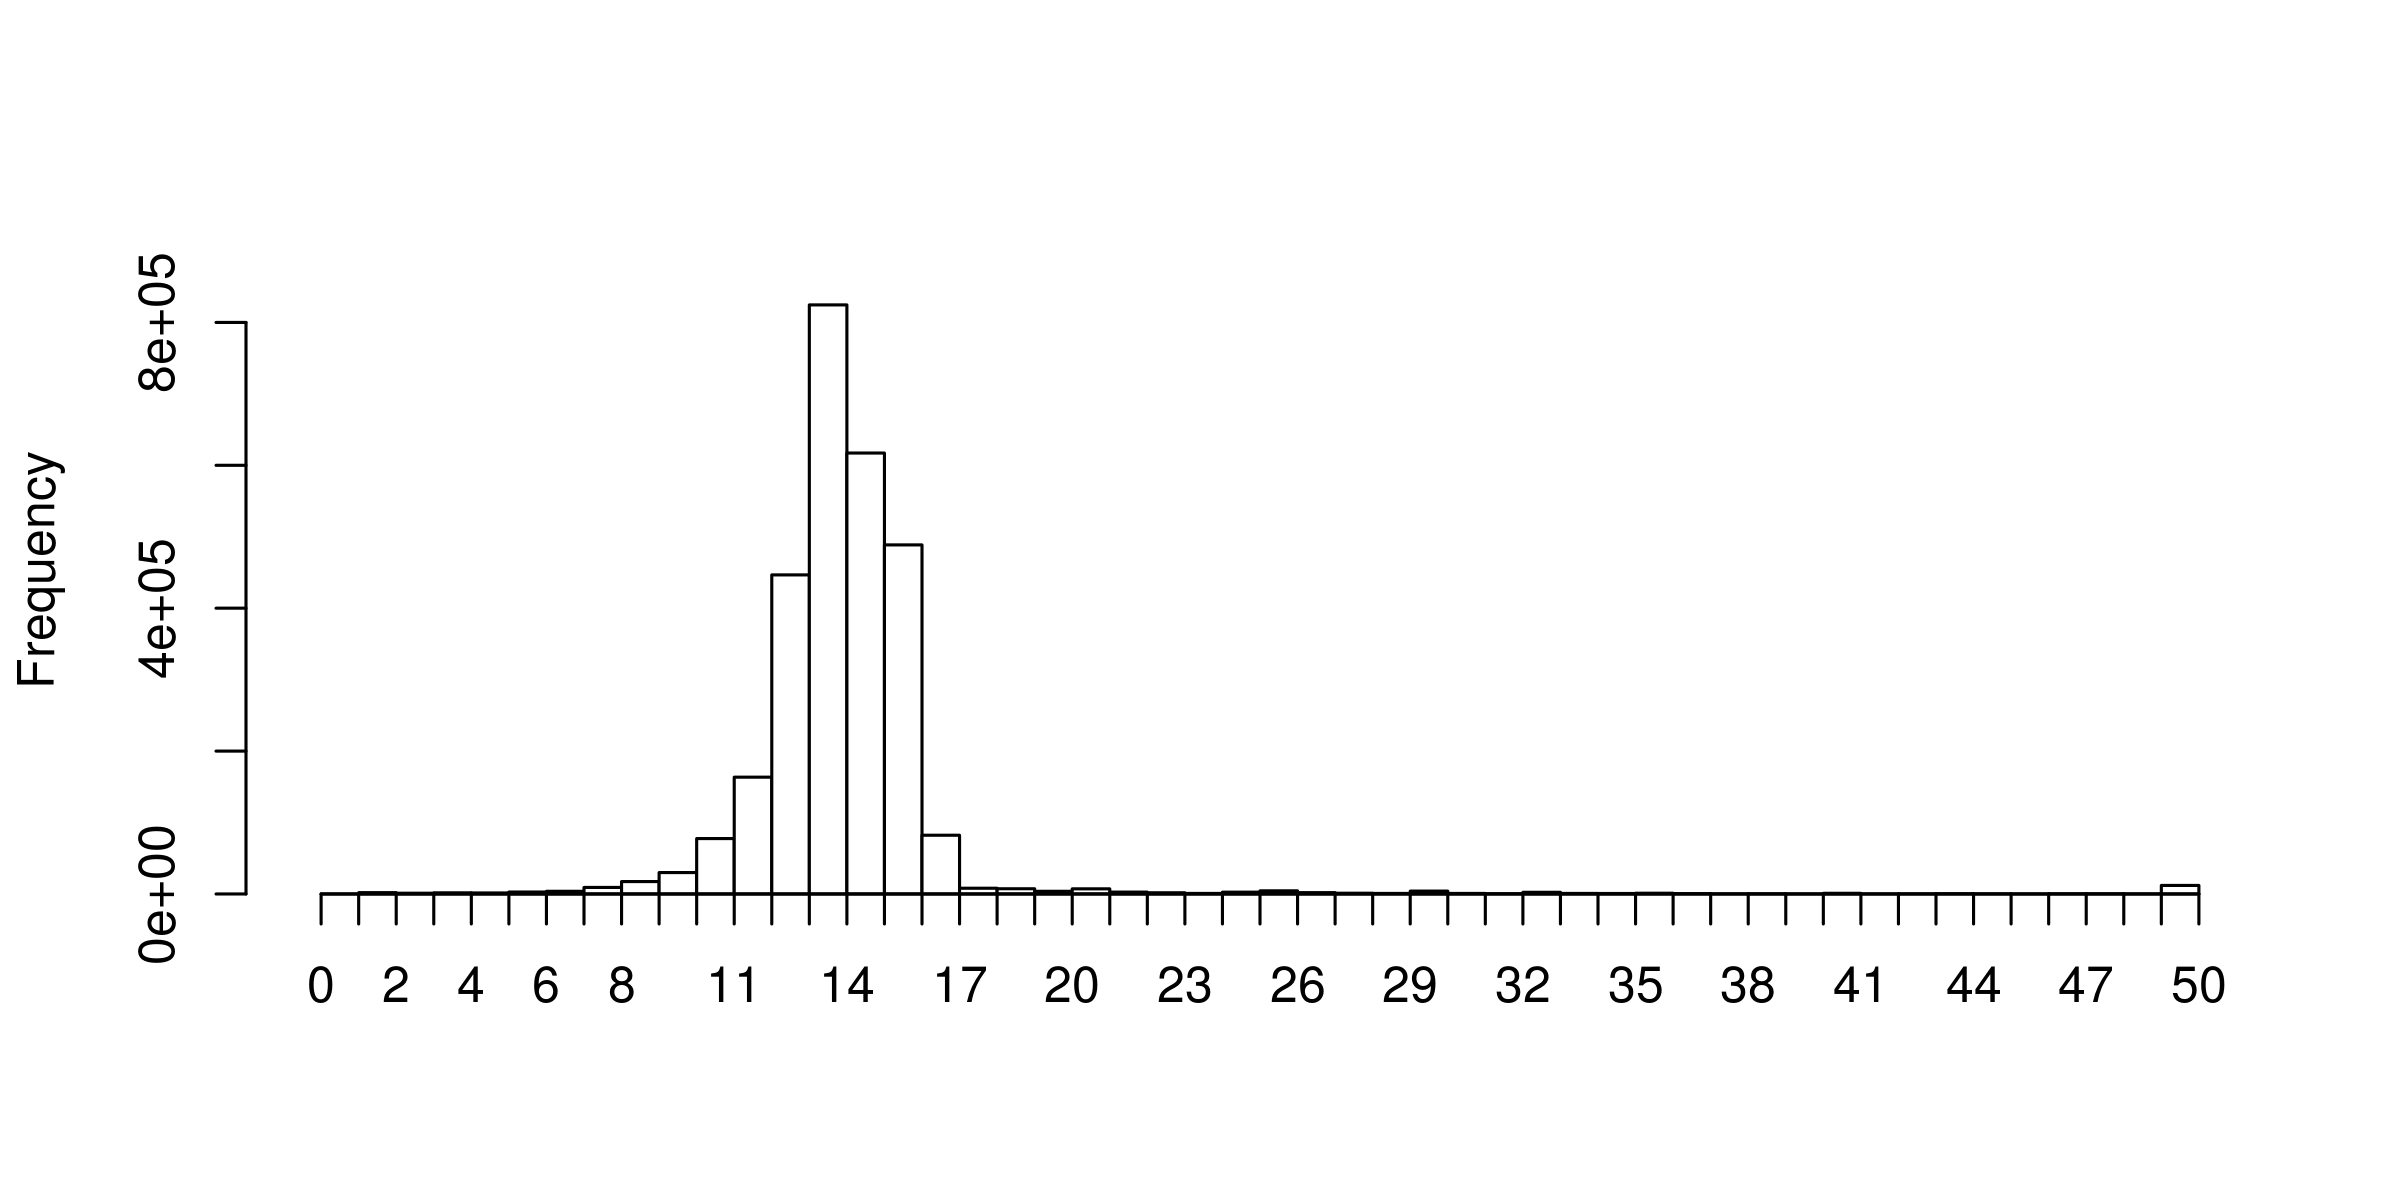
\includegraphics[width=0.8\textwidth]{de_novo/velvet/velvet_Rplot001.png}
\caption{\label{fig:SRS004748_coverage_hist} A weighted k-mer coverage histogram of the single-end reads.}
\end{figure}

\begin{steps}
After choosing the expected coverage and the coverage cut-off, you can exit R by
typing:
\begin{lstlisting}[style=R]
q()
\end{lstlisting}
\end{steps}

\begin{steps}
The weighted histogram suggests to me that the expected coverage is around 14
and that everything below 6 is likely to be noise. Some coverage is also
represented at around 20, 30 and greater 50, which might be contamination or
repeats (depending on the dataset), but at the moment this should not worry you.
To see the improvements, rerun \texttt{velvetg} first with \texttt{-cov\_cutoff} 6 and
after checking the N50 use only / add \texttt{-exp\_cov} 14 to the command line
option. Also keep a copy of the contigs file for comparison:
\begin{lstlisting}
cd ~/NGS/velvet/part1/SRS004748
time velvetg run_25 -cov_cutoff 6

# Make a copy of the run
cp run_25/contigs.fa run_25/contigs.fa.1

time velvetg run_25 -exp_cov 14
cp run_25/contigs.fa run_25/contigs.fa.2

time velvetg run_25 -cov_cutoff 6 -exp_cov 14
cp run_25/contigs.fa run_25/contigs.fa.3
\end{lstlisting}
\end{steps}

\begin{questions}
What is the N50 with no parameter:
\begin{answer}
4,447 bp
\end{answer}

What is the N50 with \texttt{-cov\_cutoff} 6:
\begin{answer}
5,168 bp
\end{answer}

What is the N50 with \texttt{-exp\_cov} 14:
\begin{answer}
4,903 bp
\end{answer}

What is the N50 with \texttt{-cov\_cutoff} 6 \texttt{-exp\_cov} 14:
\begin{answer}
5,417 bp
\end{answer}

Did you notice a variation in the time \texttt{velvetg} took to run? If so, can you
explain why that might be?
\begin{answer}
Velvet reuses already calculated results (from PreGraph,Graph)
\end{answer}

\end{questions}

\begin{steps}
You were running \texttt{velvetg} with the \texttt{-exp\_cov} and
\texttt{-cov\_cutoff} parameters. Now try to experiment using different
cut-offs, expected parameters and also explore other settings (e.g.
\texttt{-max\_coverage}, \texttt{-max\_branch\_length}, \texttt{-unused\_reads},
\texttt{-amos\_file}, \texttt{-read\_trkg} or see \texttt{velvetg} help menu).
\end{steps}

\begin{questions}
Make some notes about the parameters you've played with and the results you
obtained.
\begin{answer}
-max\_coverage: cut-off value for the upper range (like cov\_cutoff for the lower range)\\
-max\_branch\_length: length of branch to look for bubble\\
-unused\_reads: write unused reads into file\\
-amos\_file: write AMOS message file\\
-read\_trkg: tracking read (more memory usage) - automatically on for certain operations\\
\end{answer}
\\
\\
\\
\\
\end{questions}

\subsection{AMOS Hawkeye}

The \texttt{-amos\_file} argument tells \texttt{velvetg} to output the assembly
as an AMOS message file (\texttt{*.afg}) which can then be used by tools like
Hawkeye from the AMOS suite of tools.

\begin{steps}
Lets create the AMOS message file by running \texttt{velvetg} with some
appropriate parameters:
\begin{lstlisting}
velvetg run_25 -cov_cutoff 6 -exp_cov 14 -amos_file yes
\end{lstlisting}

\begin{note}
The \texttt{-exp\_cov} argument to enable read-tracking \texttt{-read\_trkg yes} in Velvet.
Without read tracking enabled, very little read-level information can be output
to the AMOS message file. This results in a pretty useless visualisation in
Hawkeye! However, since reads are being tracked, the analysis takes longer and
uses more memory.
\end{note}

Now convert the AMOS message file \texttt{velvet\_asm.afg} into an AMOS bank
using \texttt{bank-transact} and view the assembly with AMOS Hawkeye.
\begin{lstlisting}
bank-transact -c -b run_25/velvet_asm.bnk -m run_25/velvet_asm.afg
hawkeye run_25/velvet_asm.bnk
\end{lstlisting}

Have a look around the interface, in particular try to look at the ``Scaffold
View'' and ``Contig View'' of the larges scaffold. You should see something like
this:

\begin{figure}[H]
\centering
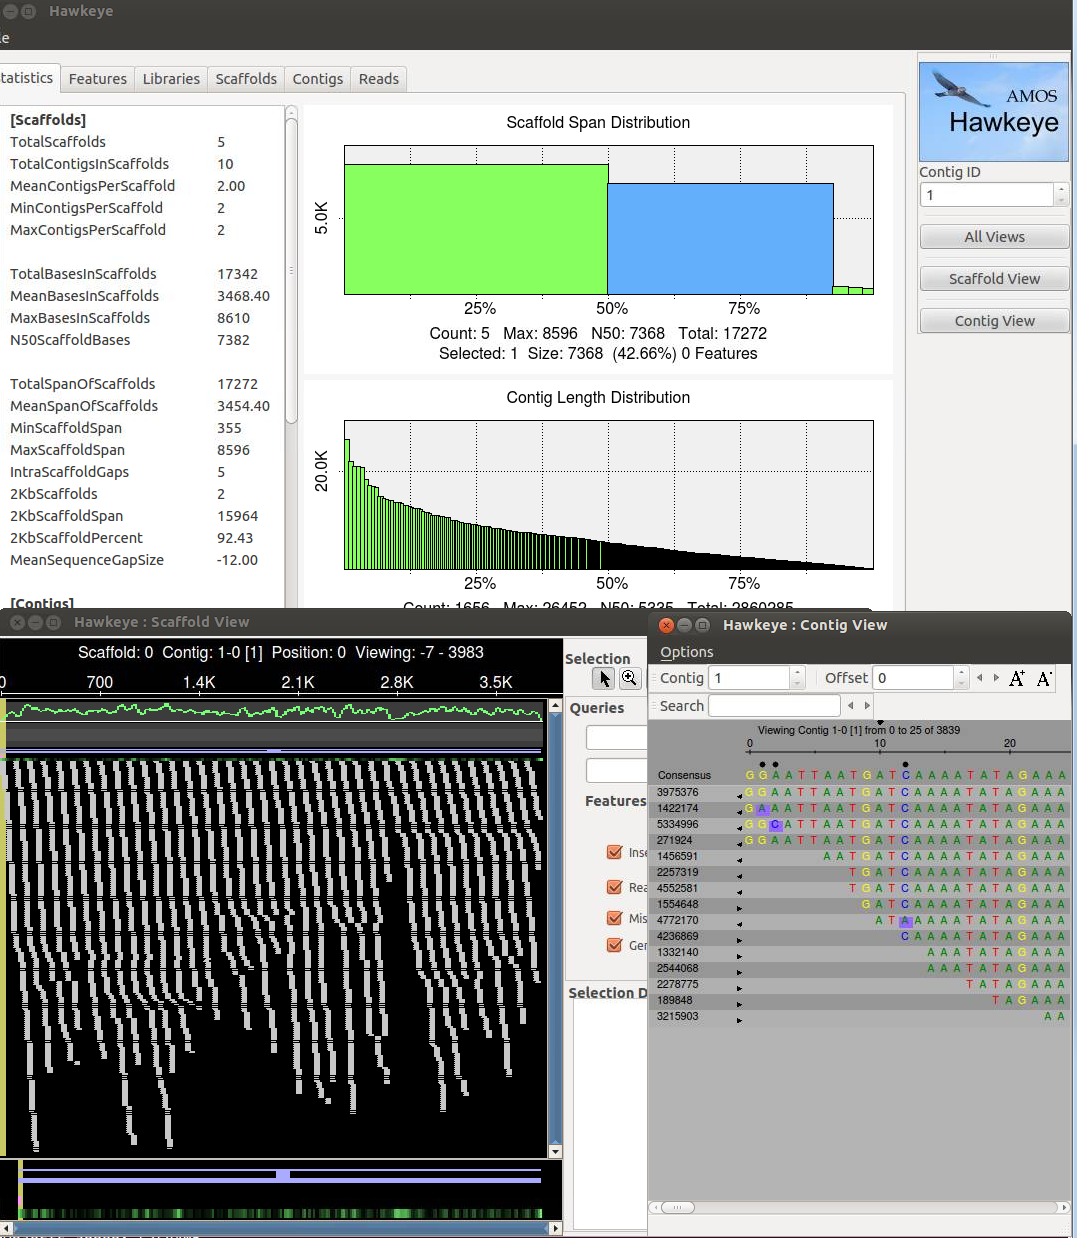
\includegraphics[width=0.8\textwidth]{de_novo/velvet/hawkeye_single_ended.png}
\caption{\label{fig:hawkeye_single_ended}}
\end{figure}

\end{steps}

\begin{bonus}
If you have time, try running the \texttt{velvetg} command without the
\texttt{-exp\_cov} argument, create the AMOS bank and see how the assemblies
look different in Hawkeye. Here's a hint:
\begin{lstlisting}
velvetg run_25 -cov_cutoff 6 -amos_file yes
bank-transact -c -b run_25/velvet_asm.bnk -m run_25/velvet_asm.afg
hawkeye run_25/velvet_asm.bnk
\end{lstlisting}

\end{bonus}

\begin{advanced}
\subsection{Simple Assembly Simulation}

\begin{note}
The data for this section is from Staphylococcus aureus MRSA252, a genome
closely related to the genome that provided the short read data in the earlier
sections of this exercise. The sequence data this time is the fully assembled
genome. The genome size is therefore known exactly and is 2,902,619 bp.
\end{note}

\begin{information}
In this exercise you will process the single whole genome sequence with \texttt{velveth}
and \texttt{velvetg}, look at the output only and go no further. The main intent of
processing this whole genome is to compute its N50 value. This must clearly be
very close to the ideal N50 value for the short reads assembly and so aid
evaluation of that assembly.
\end{information}

\begin{steps}
To begin, move back to the main directory for this exercise, make a
sub-directory for the processing of this data and move into it. All in one go,
this would be:
\begin{lstlisting}
cd ~/NGS/velvet/part1/ 
mkdir MRSA252 
cd MRSA252
\end{lstlisting}

Next, you need to download the genome sequence from
\url{http://www.ensemblgenomes.org/} which holds five new sites, for bacteria,
protists, fungi, plants and invertebrate metazoa. You could browse for the data
you require or use the file which we have downloaded for you. For the easier of
these options, make and check a symlink to the local file and with the
commands:
\begin{lstlisting}
ln -s ~/NGS/Data/s_aureus_mrsa252.EB1_s_aureus_mrsa252.dna.chromosome.Chromosome.fa.gz ./
ls -l
\end{lstlisting}

\end{steps}

\begin{note}
Usually Velvet expects relatively short sequence entries and for this reason has
a read limit of 32,767 bp per sequence entry. As the genome size is 2,902,619 bp
- longer as the allowed limit and does not fit with the standard settings into
velvet. But like the maximum k-mer size option, you can tell Velvet during
compile time, using \texttt{LONGSEQUENCES=Y}, to expect longer input sequences
than usual. I already prepared the executable which you can use by typing
\texttt{velveth\_long} and \texttt{velvetg\_long}.
\end{note}

\begin{steps}
Now, run \texttt{velveth\_long}, using the file you either just downloaded or created a
symlink to as the input:
\begin{lstlisting}
velveth_long run_25 25 -fasta.gz -long s_aureus_mrsa252.EB1_s_aureus_mrsa252.dna.chromosome.Chromosome.fa.gz
velvetg_long run_25
\end{lstlisting}

\end{steps}

\begin{questions}
What is the N50?
\begin{answer}
24,142 bp
\end{answer}

How does the N50 compare to the previous single end run (SRS004748)?
\begin{answer}
Big difference
\end{answer}
  
Does the total length differ from the input sequence length?
\begin{answer}
2,817,181 (stats) vs 2,902,619 (input)
\end{answer}
  
What happens when you rerun velvet with a different k-mer length?
\begin{answer}
K-mer 31: N50: 30,669 bp, total 2,822,878
\end{answer}

\end{questions}
\end{advanced}


\section{Assembling Paired-end Reads}

The use of paired-end data in \textit{de novo} genome assembly results in better
quality assemblies, particularly for larger, more complex genomes. In addition,
paired-end constraint violation (expected distance and orientation of paired
reads) can be used to identify misassemblies.

\begin{warning}
If you are doing \textit{de novo} assembly, pay the extra and get paired-ends:
they're worth it!
\end{warning}

\begin{note}
The data you will examine in this exercise is again from Staphylococcus aureus
which has a genome of around 3MBases. The reads are Illumina paired end with an
insert size of $~$350 bp.

The required data can be downloaded from the SRA. Specifically, the run data
(SRR022852) from the SRA Sample SRS004748.

\center{\url{http://www.ebi.ac.uk/ena/data/view/SRS004748}}

\end{note}

\begin{information}
The following exercise focuses on preparing the paired-end FASTQ files ready for
Velvet, using Velvet in paired-end mode and comparing results with Velvet's
'auto' option.
\end{information}

\begin{steps}
First move to the directory you made for this exercise and make a suitable named
directory for the exercise:
\begin{lstlisting}
cd ~/NGS/velvet/part2 
mkdir SRS004748 
cd SRS004748
\end{lstlisting}

There is no need to download the read files, as they are already stored
locally. You will simply create a symlink to this pre-downloaded data using
the following commands:
\begin{lstlisting}
ln -s ~/NGS/Data/SRR022852_?.fastq.gz ./
\end{lstlisting}

It is interesting to monitor the computer's resource utilisation, particularly
memory. A simple way to do this is to open a second terminal and in it type:
\begin{lstlisting}
top
\end{lstlisting}
\end{steps}

\begin{note}
\texttt{top} is a program that continually monitors all the processes running on
your computer, showing the resources used by each. Leave this running and refer
to it periodically throughout your Velvet analyses. Particularly if they are
taking a long time or whenever your curiosity gets the better of you. You should
find that as this practical progresses, memory usage will increase
significantly.

Now, back to the first terminal, you are ready to run \texttt{velveth} and
\texttt{velvetg}. The reads are \texttt{-shortPaired} and for the
first run you should not use any parameters for \texttt{velvetg}.
\end{note}

\begin{information}
From this point on, where it will be informative to time
your runs. This is very easy to do, just prefix the command to run the program
with the command \texttt{time}. This will cause UNIX to report how long the program took
to complete its task.
\end{information}

\begin{steps}
Set the two stages of velvet running, whilst you watch the memory usage as
reported by \texttt{top}. Time the \texttt{velvetg} stage:
\begin{lstlisting}
velveth run_25 25 -fmtAuto -create_binary -shortPaired -separate SRR022852_1.fastq.gz SRR022852_2.fastq.gz
time velvetg run_25
\end{lstlisting}

\end{steps}

\begin{questions}
What does \texttt{-fmtAuto} and \texttt{-create\_binary} do? (see help menu)
\begin{answer}
\texttt{-fmtAuto} tries to detect the correct format of the input files e.g.
  FASTA, FASTQ and whether they are compressed or not.

\texttt{-create\_binary} outputs sequences as a binary file. That means that
  \texttt{velvetg} can read the sequences from the binary file more quickly that
  from the original sequence files.
\end{answer}

Comment on the use of memory and CPU for \texttt{velveth} and \texttt{velvetg}?
\begin{answer}
\texttt{velveth} uses only one CPU while \texttt{velvetg} uses all possible CPUs
for some parts of the calculation.
\end{answer}
 
How long did \texttt{velvetg} take?
\begin{answer}
My own measurements are:\\
\texttt{real    1m8.877s; user    4m15.324s; sys     0m4.716s}
\end{answer}

\end{questions}

\begin{steps}
Next, after saving your \texttt{contigs.fa} file from being overwritten, set the
cut-off parameters that you investigated in the previous exercise and rerun
\texttt{velvetg}.
time and monitor the use of resources as previously. Start with
\texttt{-cov\_cutoff 16} thus:
\begin{lstlisting}
mv run_25/contigs.fa run_25/contigs.fa.0
time velvetg run_25 -cov_cutoff 16
\end{lstlisting}

Up until now, \texttt{velvetg} has ignored the paired-end information. Now try
running \texttt{velvetg} with both \texttt{-cov\_cutoff 16} and
\texttt{-exp\_cov 26}, but first save your \texttt{contigs.fa} file. By using
\texttt{-cov\_cutoff} and \texttt{-exp\_cov}, \texttt{velvetg} tries to estimate
the insert length, which you will see in the \texttt{velvetg} output. The
command is, of course:
\begin{lstlisting}
mv run_25/contigs.fa run_25/contigs.fa.1
time velvetg run_25 -cov_cutoff 16 -exp_cov 26
\end{lstlisting}

\end{steps}

\begin{questions}
Comment on the time required, use of memory and CPU for \texttt{velvetg}?
\begin{answer}
Runtime is lower when velvet can reuse previously calculated data. By using
\texttt{-exp\_cov}, the memory usage increases.
\end{answer}

Which insert length does Velvet estimate?
\begin{answer}
Paired-end library 1 has length: 228, sample standard deviation: 26
\end{answer}

\end{questions}

\begin{steps}
Next try running \texttt{velvetg} in `paired-end mode`. This entails running \texttt{velvetg}
specifying the insert length with the parameter \texttt{-ins\_length} set to 350. Even
though velvet estimates the insert length it is always advisable to check /
provide the insert length manually as velvet can get the statistics wrong due
to noise. Just in case, save your last version of \texttt{contigs.fa}. The commands are:
\begin{lstlisting}
mv run_25/contigs.fa run_25/contigs.fa.2
time velvetg run_25 -cov_cutoff 16 -exp_cov 26 -ins_length 350
mv run_25/contigs.fa run_25/contigs.fa.3
\end{lstlisting}
\end{steps}

\begin{questions}
How fast was this run?
\begin{answer}
My own measurements are:\\
\texttt{real    0m29.792s; user    1m4.372s; sys     0m3.880s}
\end{answer}

\end{questions}

\begin{steps}
Take a look into the Log file.
\end{steps}

\begin{questions}
What is the N50 value for the \texttt{velvetg} runs using the switches:\\
\begin{answer}
Base run: 19,510 bp
\end{answer}
\texttt{-cov\_cutoff 16}
\begin{answer}
24,739 bp
\end{answer}

\texttt{-cov\_cutoff 16 -exp\_cov 26}
\begin{answer}
61,793 bp
\end{answer}

\texttt{-cov\_cutoff 16 -exp\_cov 26 -ins\_length 350}
\begin{answer}
n50 of 62,740 bp; max 194,649 bp; total 2,871,093 bp
\end{answer}

\end{questions}

\begin{steps}
Try giving the \texttt{-cov\_cutoff} and/or \texttt{-exp\_cov} parameters the
value \texttt{auto}. See the \texttt{velvetg} help to show you how. The
information Velvet prints during running includes information about the values
used (coverage cut-off or insert length) when using the \texttt{auto} option.
\end{steps}

\begin{questions}
What coverage values does Velvet choose (hint: look at the output that Velvet
produces while running)?
\begin{answer}
Median coverage depth = 26.021837\\
Removing contigs with coverage $<$ 13.010918 \ldots
\end{answer}

How does the N50 value change?
\begin{answer}
n50 of 68,843 bp; max 194,645 bp; total 2,872,678 bp
\end{answer}
\end{questions}

\begin{steps}
Run \texttt{gnx} on all the \texttt{contig.fa} files you have generated in the
course of this exercise. The command will be:
\begin{lstlisting}
gnx -min 100 -nx 25,50,75 run_25/contigs.fa*
\end{lstlisting}
\end{steps}

\begin{questions}
For which runs are there Ns in the \texttt{contigs.fa} file and why? 
\begin{answer}
contigs.fa.2, contigs.fa.3, contigs.fa\\
Velvet tries to use the provided (or infers) the insert length and fills
ambiguous regions with Ns.
\end{answer}

Comment on the number of contigs and total length generated for each run.
\begin{answer}
\begin{table}[H]
  %\centering
    \begin{tabular}{llll}
    \toprule
    Filename & No. contigs & Total length & No. Ns \\
    \midrule
    Contigs.fa.0 & 631 & 2,830,659 & 0 \\
    Contigs.fa.1 & 580 & 2,832,670 & 0 \\
    Contigs.fa.2 & 166 & 2,849,919 & 4,847 \\
    Contigs.fa.3 & 166 & 2,856,795 & 11,713 \\
    Contigs.fa & 163 & 2,857,439 & 11,526 \\
    \bottomrule
    \end{tabular}%
  \caption{\label{tab:velvetrunresults}}%
\end{table}%
\end{answer}
\end{questions}

\subsection{AMOS Hawkeye}

We will now output the assembly in the AMOS massage format and visualise the
assembly using AMOS Hawkeye.

\begin{steps}
Run \texttt{velvetg} with appropriate arguments and output the AMOS message
file, then convert it to an AMOS bank and open it in Hawkeye:
\begin{lstlisting}
time velvetg run_25 -cov_cutoff 16 -exp_cov 26 -ins_length 350 -amos_file yes -read_trkg yes 
time bank-transact -c -b run_25/velvet_asm.bnk -m run_25/velvet_asm.afg         
hawkeye run_25/velvet_asm.bnk
\end{lstlisting}
\end{steps}

\begin{questions}
Looking at the scaffold view of a contig, comment on the proportion of ``happy
mates'' to ``compressed mates'' and ``stretched mates''.
\begin{answer}
Nearly all mates are compressed with no stretched mates and very few happy
mates.
\end{answer}

What is the mean and standard deviation of the insert size reported under the
Libraries tab?
\begin{answer}
Mean: 350 bp
SD: 35 bp
\end{answer}

Look at the actual distribution of insert sizes for this library. Can you
explain where there is a difference between the mean and SD reported in those
two places?
\begin{answer}
We specified \texttt{-ins\_length 350} to the \texttt{velvetg} command. Velvet
uses this value, in the AMOS message file that it outputs, rather than its own
estimate.
\end{answer}
\end{questions}

\begin{steps}
You can get AMOS to re-estimate the mean and SD of insert sizes using
intra-contig pairs. First, close Hawkeye and then run the following commands
before reopening the AMOS bank to see what has changed.
\begin{lstlisting}
asmQC -b run_25/velvet_asm.bnk -scaff -recompute -update -numsd 2
hawkeye run_25/velvet_asm.bnk
\end{lstlisting}
\end{steps}

\begin{questions}
Looking at the scaffold view of a contig, comment on the proportion of ``happy
mates'' to ``compressed mates'' and ``stretched mates''.
\begin{answer}
There are only a few compressed and stretched mates compared to happy mates.
There are similar numbers of stretched and compressed mates.
\end{answer}

What is the mean and standard deviation of the insert size reported under the
Libraries tab?
\begin{answer}
TODO
Mean: 226 bp
SD: 25 bp
\end{answer}

Look at the actual distribution of insert sizes for this library. Does the mean
and SD reported in both places now match?
\begin{answer}
Yes
\end{answer}

Can you find a region with an unusually high proportion of stretched, compressed,
incorrectly orientated or linking mates? What might this situation indicate?
\begin{answer}
This would indicate a possible misassembly and worthy of further investigation.

Look at the largest scaffold, there are stacks of stretched pairs which span
contig boundaries. This indicates that the gap size has been underestimated
during the scaffolding phase.
\end{answer}
\end{questions}


\subsection{Velvet and Data Quality}
So far we have used the raw read data without performing any quality control or
read trimming prior to doing our velvet assemblies.

\begin{warning}
Velvet does not use quality information present in FASTQ files.
\end{warning}

For this reason, it is vitally important to perform read QC and quality
trimming. In doing so, we remove errors/noise from the dataset which in turn
means velvet will run faster, will use less memory and will produce a better
assembly. Assuming we haven't compromised too much on coverage.

\begin{information}
To investigate the effect of data quality, we will use the run data (SRR023408)
from the SRA experiment SRX008042. The reads are Illumina paired end with an
insert size of 92 bp.
\end{information}

\begin{steps}
Go back to the main directory for this exercise and create and enter a new
directory dedicated to this phase of the exercise. The commands are:
\begin{lstlisting}
cd ~/NGS/velvet/part2 
mkdir SRX008042 
cd SRX008042
\end{lstlisting}

Create symlinks to the read data files that we downloaded for you from the SRA:
\begin{lstlisting}
ln -s ~/NGS/Data/SRR023408_?.fastq.gz ./
\end{lstlisting}
\end{steps}

\begin{note}
We will use FastQC, a tool you should be familiar with, to visualise the quality
of our data. We will use FastQC in the Graphical User Interface (GUI) mode.
\end{note}

\begin{steps}
Start FastQC and set the process running in the background, by using a trailing
\texttt{\&}, so we get control of our terminal back for entering more commands:
\begin{lstlisting}
fastqc &
\end{lstlisting}
\end{steps}

\begin{steps}
Open the two compressed FASTQ files (File $->$ Open) by selecting them both and clicking OK).
Look at tabs for both files:
\end{steps}

\begin{figure}[H]
\centering
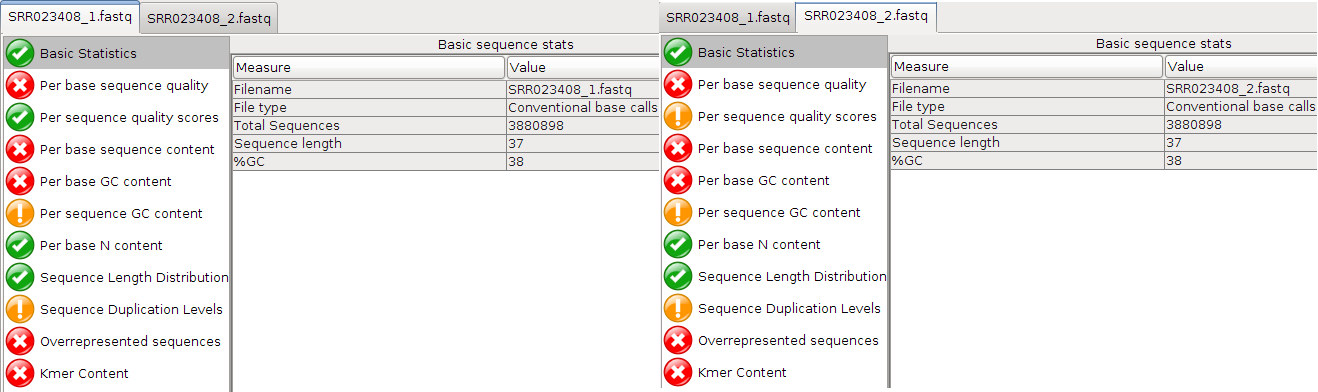
\includegraphics[width=0.8\textwidth]{de_novo/velvet/paired_fastqc.png}
\caption{\label{fig:paired_fastqc}}
\end{figure}

\begin{questions}
Are the quality scores the same for both files?
\begin{answer}
Overall yes
\end{answer}

Which value varies?
\begin{answer}
Per sequence quality scores
\end{answer}

Take a look at the Per base sequence quality for both files. Did you note that
it is not good for either file?
\begin{answer}
The quality score of both files drop very fast. Qualities of the REV strand drop
faster than the FWD strand. This is because the template has been sat around
while the FWD strand was sequenced.
\end{answer}

At which positions would you cut the reads if we did ``fixed length trimming''?
\begin{answer}
Looking at the ``Per base quality" and ``Per base sequence content'', I would
choose around 27
\end{answer}

Why does the quality deteriorate towards the end of the read?
\begin{answer}
Errors more likely for later cycles
\end{answer}

Does it make sense to trim the 5' start of reads?
\begin{answer}
Looking at the ``Per base sequence content", yes - there is a clear signal at the beginning.
\end{answer}
\end{questions}

\begin{steps}
Have a look at the other options that FastQC offers.
\end{steps}

\begin{questions}
Which other statistics could you use to support your trimming strategy?
\begin{answer}
``Per base sequence content", ``Per base GC content", ``Kmer content", ``Per
base sequence quality"
\end{answer}
\end{questions}

\begin{figure}[H]
\centering
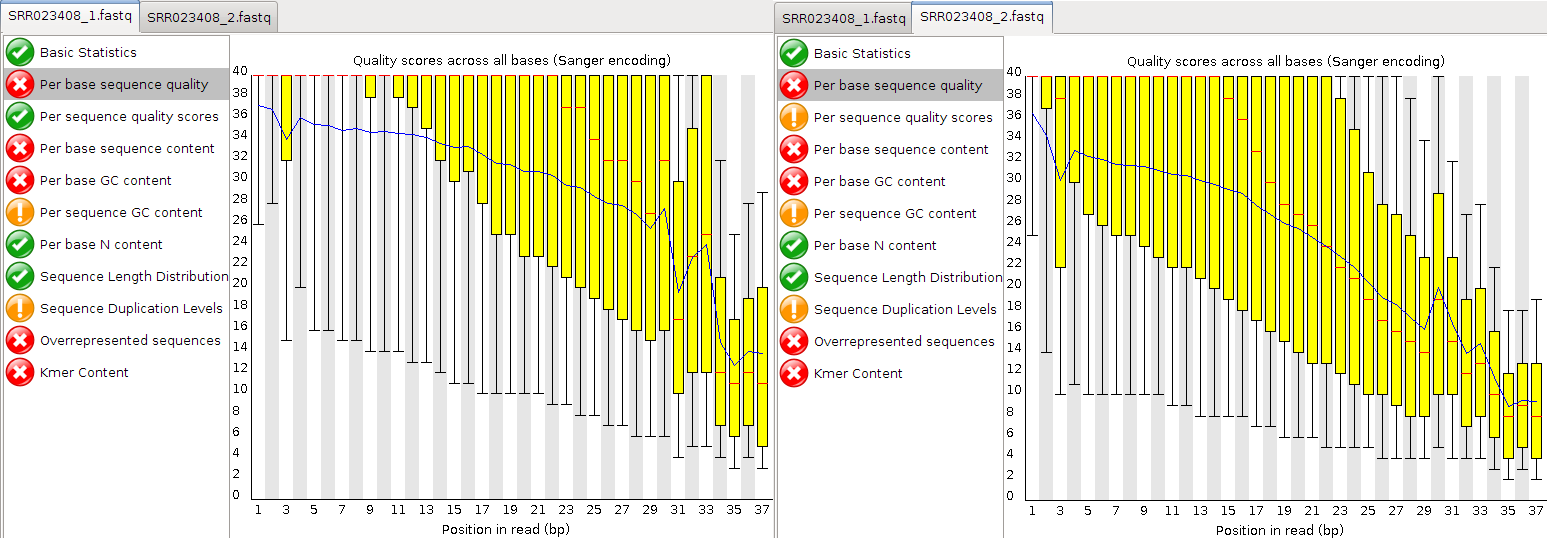
\includegraphics[width=0.8\textwidth]{de_novo/velvet/paired_fastqc_quality_plots.png}
\caption{\label{fig:paired_fastqc_quality_plots}}
\end{figure}

\begin{steps}
Once you have decided what your trim points will be, close FastQC.
We will use \texttt{fastx\_trimmer} from the FASTX-Toolkit to perform
fixed-length trimming. For usage information see the help:
\begin{lstlisting}
fastx_trimmer -h
\end{lstlisting}

\begin{note}
\texttt{fastx\_trimmer} is not able to read compressed FASTQ files, so we first
need to decompress the files ready for input.
\end{note}

The suggestion (hopefully not far from your own thoughts?) is that you trim your
reads as follows:

\begin{lstlisting}
gunzip < SRR023408_1.fastq.gz > SRR023408_1.fastq
gunzip < SRR023408_2.fastq.gz > SRR023408_2.fastq
fastx_trimmer -Q 33 -f 1 -l 32 -i SRR023408_1.fastq -o SRR023408_trim1.fastq 
fastx_trimmer -Q 33 -f 1 -l 27 -i SRR023408_2.fastq -o SRR023408_trim2.fastq
\end{lstlisting}

\begin{advanced}
Many NGS read files are large. This means that simply reading and writing files
can become the bottleneck, also known as I/O bound. Therefore, it is often good practice to
avoid unnecessary disk read/write.

We could do what is called pipelining to send a stream of data from one command
to another, using the pipe (\texttt{|}) character, without the need for
intermediary files. The following command would achieve this:
\begin{lstlisting}
gunzip --to-stdout < SRR023408_1.fastq.gz | fastx_trimmer -Q 33 -f 4 -l 32 -o SRR023408_trim1.fastq 
gunzip --to-stdout < SRR023408_2.fastq.gz | fastx_trimmer -Q 33 -f 3 -l 29 -o SRR023408_trim2.fastq
\end{lstlisting}
\end{advanced}

Now run \texttt{velveth} with a k-mer value of 21 for both the untrimmed and
trimmed read files in \texttt{-shortPaired} mode. Separate the output of the two
executions of \texttt{velveth} into suitably named directories, followed by
\texttt{velvetg}:
\begin{lstlisting}
# untrimmed reads
velveth run_21 21 -fmtAuto -create_binary -shortPaired -separate SRR023408_1.fastq SRR023408_2.fastq
time velvetg run_21

# trimmed reads
velveth run_21trim 21 -fmtAuto -create_binary -shortPaired -separate SRR023408_trim1.fastq SRR023408_trim2.fastq
time velvetg run_21trim
\end{lstlisting}
\end{steps}

\begin{questions}
How long did the two \texttt{velvetg} runs take?
\begin{answer}
run\_25:      \texttt{real    3m16.132s; user    8m18.261s; sys     0m7.317s}\\
run\_25trim:  \texttt{real    1m18.611s; user    3m53.140s; sys     0m4.962s}
\end{answer}

What N50 scores did you achieve?
\begin{answer}
Untrimmed: 11\\
Trimmed: 15
\end{answer}

What were the overall effects of trimming?
\begin{answer}
Time saving, increased N50, reduced coverage
\end{answer}
\end{questions}

\begin{steps}
The evidence is that trimming improved the assembly. The thing to do surely, is
to run \texttt{velvetg} with the \texttt{-cov\_cutoff} and \texttt{-exp\_cov}. In order
to use \texttt{-cov\_cutoff} and \texttt{-exp\_cov} sensibly, you need to
investigate with R, as you did in the previous exercise, what parameter values
to use. Start up R and produce the weighted histograms:
\begin{lstlisting}[style=R]
R --no-save
library(plotrix) 
data <- read.table("run_21/stats.txt", header=TRUE) 
data2 <- read.table("run_21trim/stats.txt", header=TRUE) 
par(mfrow=c(1,2))
weighted.hist(data$short1_cov, data$lgth, breaks=0:50)
weighted.hist(data2$short1_cov, data2$lgth, breaks=0:50)
\end{lstlisting}

\begin{figure}[H]
\centering
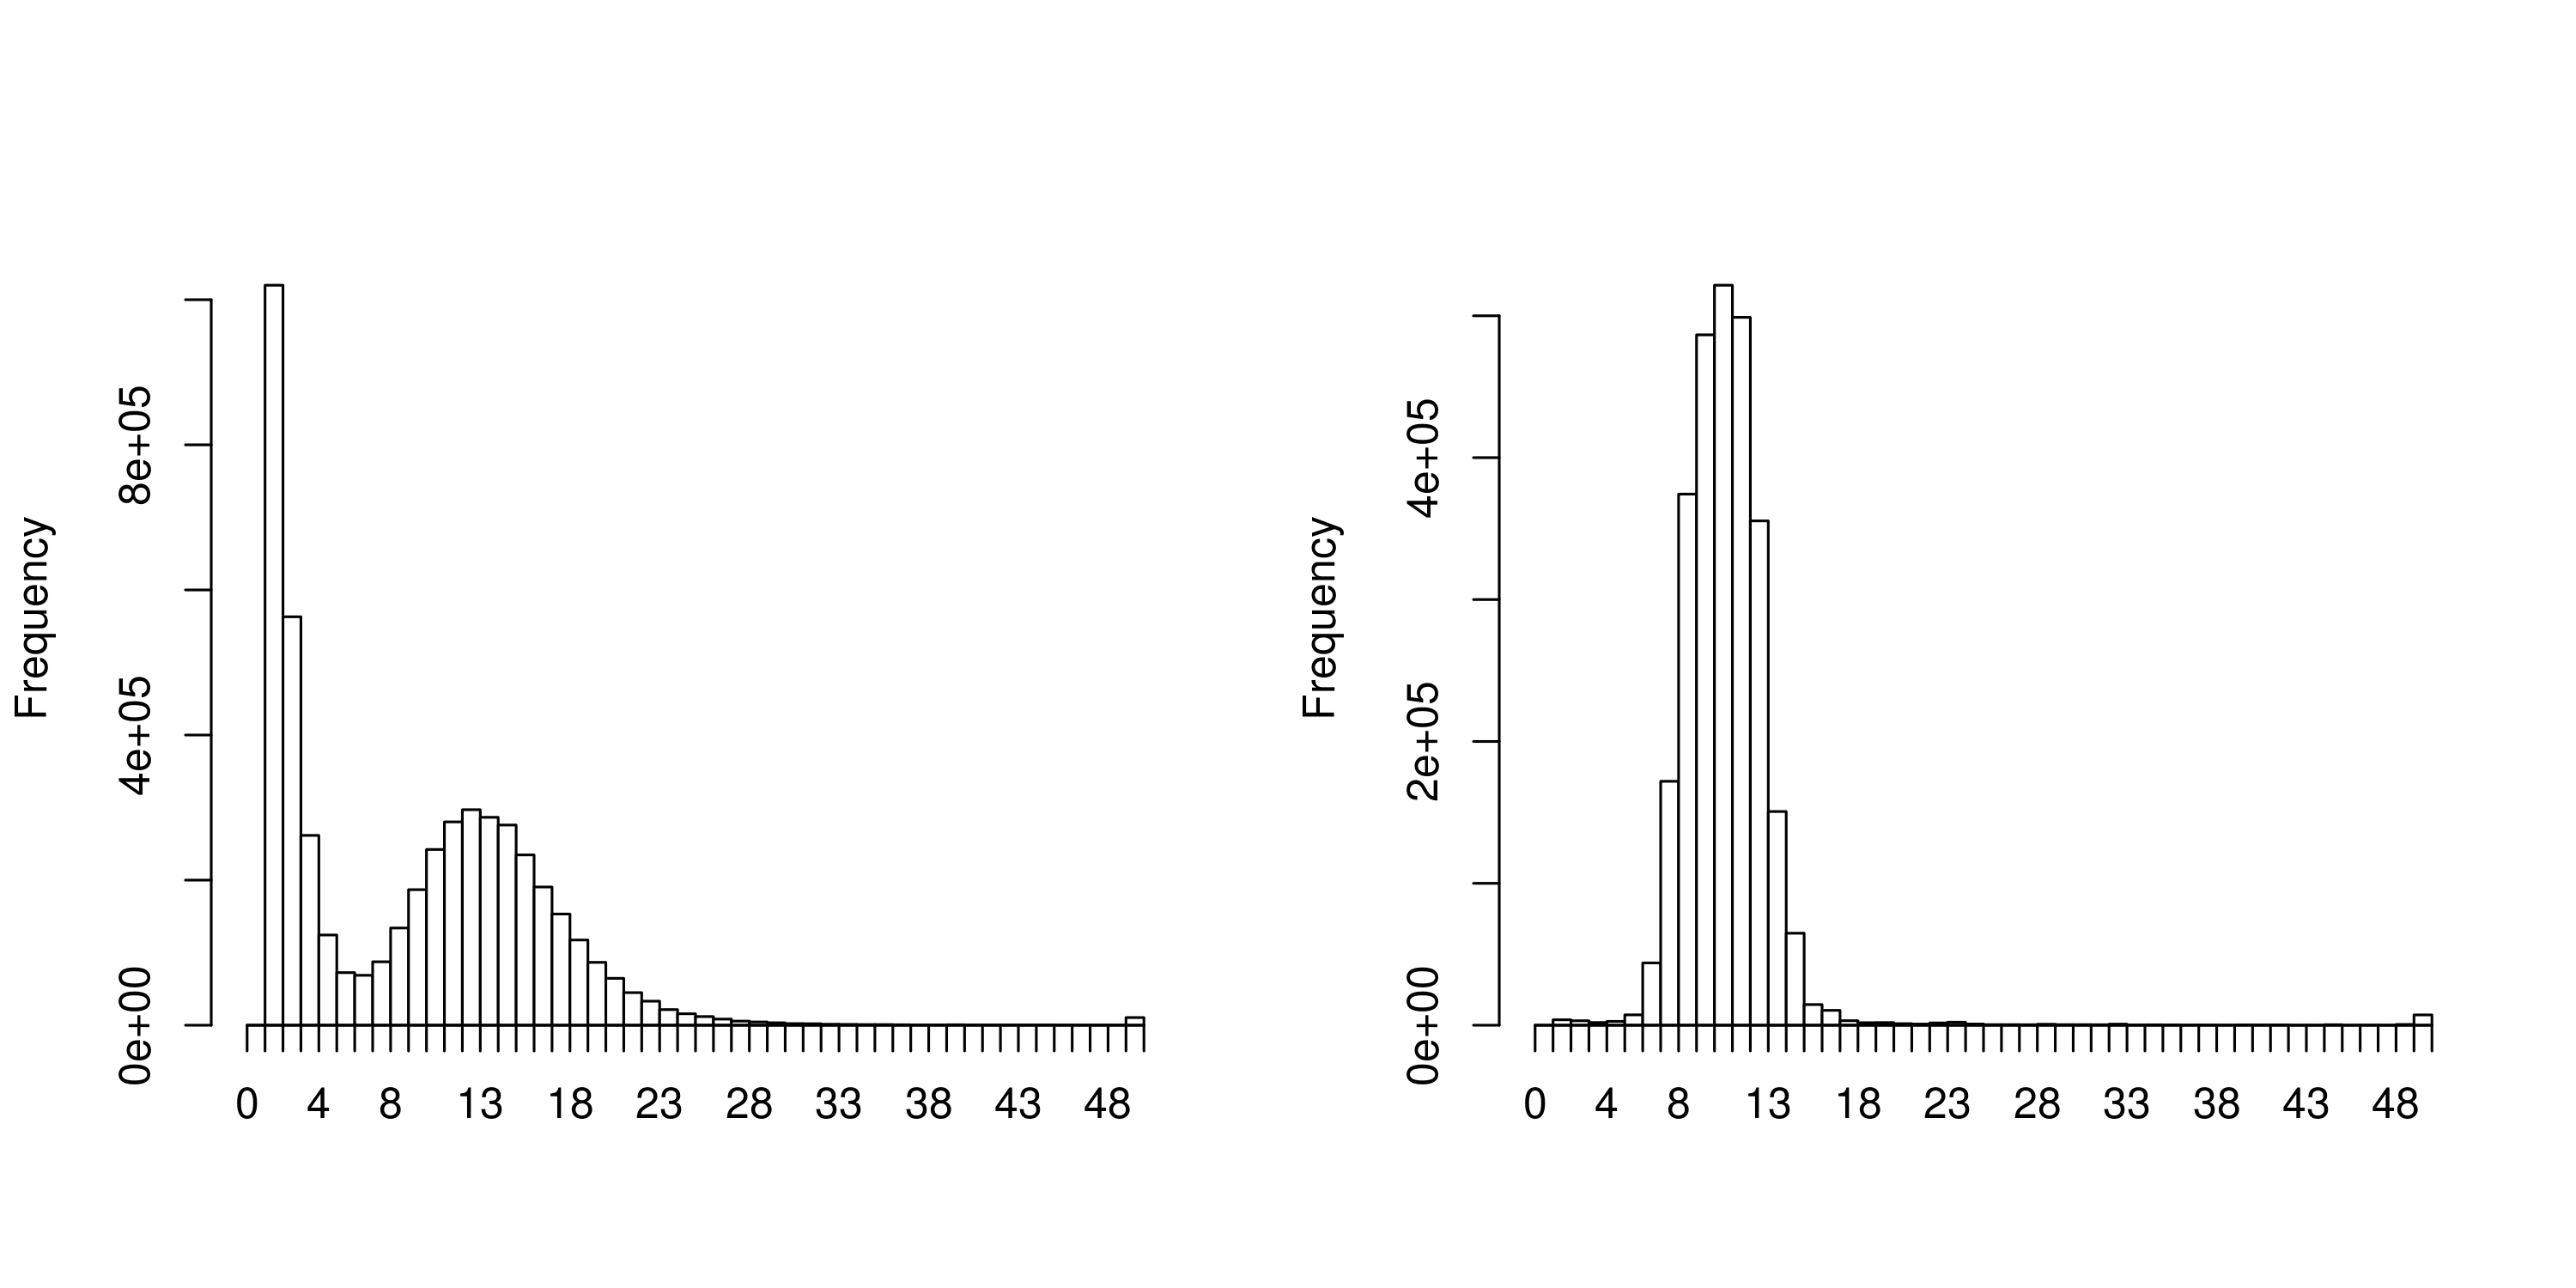
\includegraphics[width=0.8\textwidth]{de_novo/velvet/velvet_Rplot002.png}
\caption{\label{fig:velvet_Rplot002} Weighted k-mer coverage histograms of the paired-end reads pre-trimmed (left) and post-trimmed (right).}
\end{figure}

For the untrimmed read histogram (left) there is an expected coverage of around
13 with a coverage cut-off of around 7. For the trimmed read histogram (right)
there is an expected coverage of around 9 with a coverage cut-off of around 5.

If you disagree, feel free to try different settings, but first quit R before
running \texttt{velvetg}:
\begin{lstlisting}[style=R]
q()
\end{lstlisting}

\begin{lstlisting}
time velvetg run_21 -cov_cutoff 7 -exp_cov 13 -ins_length 92
time velvetg run_21trim -cov_cutoff 5 -exp_cov 9 -ins_length 92
\end{lstlisting}

\end{steps}

\begin{questions}
How good does it look now?\\
\begin{answer}
Still not great
\end{answer}
Comment on:\\ 
Runtime
\begin{answer}
Reduced runtime
\end{answer}

Memory
\begin{answer}
Lower memory usage
\end{answer}

k-mer choice (Can you use k-mer 31 for a read of length 30 bp?)
\begin{answer}
K-mer has to be lower than the read length and the K-mer coverage should be
sufficient to produce results.
\end{answer}

Does less data mean ``worse" results?
\begin{answer}
Not necessarily. If you have lots of data you can safely remove poor data
without too much impact on overall coverage.
\end{answer}
  
How would a smaller/larger k-mer size behave?
\begin{answer}
% TODO
\end{answer}
\end{questions}

\begin{steps}
Compare the results, produced during the last exercises, with each other:

\begin{table}[H]
  \centering
    \begin{tabular*}{0.9\textwidth}{l|l|l|l}
    \toprule
    Metric & SRR022852 & SRR023408 & SRR023408.trimmed \\
    \midrule
    Overall Quality (1-5) & & & \\[0.5\questionspacing]
    \hline
    bp Coverage & & & \\[0.5\questionspacing]
    \hline
    k-mer Coverage & & & \\[0.5\questionspacing]
    \hline
    N50 (k-mer used) & & & \\[0.5\questionspacing]
    \bottomrule
    \end{tabular*}
  \caption{\label{tab:comparison}}
\end{table}

\begin{answer}
\begin{table}[H]
  \centering
    \begin{tabular*}{0.9\textwidth}{l|l|l|l}
    \toprule
    Metric & SRR022852 & SRR023408 & SRR023408.trimmed \\
    \midrule
    Overall Quality (1-5) & 2 & 5 & 4\\[0.5\questionspacing]
    \hline
    bp Coverage & 136 x (36 bp;11,374,488) & 95x (37bp; 7761796) & 82x (32bp; 7761796)\\[0.5\questionspacing]
    \hline
    k-mer Coverage & 45x & 43x (21); 33x (25) & 30x (21); 20.5x (25)\\[0.5\questionspacing]
    \hline
    N50 (k-mer used) & 68,843 (25) & 2,803 (21) & 2,914 (21)\\[0.5\questionspacing]
    \bottomrule
    \end{tabular*}
  \caption{\label{tab:comparison_result}}
\end{table}
\end{answer}

\end{steps}

\begin{questions}
What would you consider as the ``best" assembly?
\begin{answer}
SRR022852
\end{answer}

If you found a candidate, why do you consider it as ``best" assembly?
\begin{answer}
Overall data quality and coverage
\end{answer}

How else might you assess the the quality of an assembly? Hint: Hawkeye.
\begin{answer}
By trying to identify paired-end constraint violations using AMOS Hawkeye.
\end{answer}
\end{questions}


%\section{Assembling Long (454) Read}

\begin{note}
The data you will examine in this exercise is again from Staphylococcus aureus
which has a genome of around 3MB. The reads are 454 single end.

The required data can be downloaded from the SRA. Specifically, the run data
(SRR000892, SRR000893) from the SRA Experiment SRX000181.

\center{\url{http://www.ebi.ac.uk/ena/data/view/SRX000181}}
\end{note}

\begin{information}
The following exercise focuses on processing 454 long reads with velvet and how
this differs compared to short reads.
\end{information}

\begin{steps}
First move to the directory you made for this exercise and make a suitable named
directory for the exercise before downloading the read files:
\begin{lstlisting}
cd ~/NGS/velvet/part3
mkdir SRX000181
cd SRX000181
\end{lstlisting}

The downloaded files can be used directly in velvet. To let velvet know that
these FASTQ files are long reads, you pass in the parameter \texttt{-long} by
using the commands:
\begin{lstlisting}
ln -s ~/NGS/Data/SRR000892.fastq.gz
ln -s ~/NGS/Data/SRR000893.fastq.gz
velveth run_25 25 -create_binary -fastq.gz -long *.fastq.gz
time velvetg run_25
\end{lstlisting}
\end{steps}

\begin{questions}
Take a look at the \texttt{stats.txt} file. Which columns are used compared to
short reads and why?
\begin{answer}
long\_cov instead of e.g. short1\_cov
\end{answer}

Which N50 do you get?
\begin{answer}
28 (k-mer N50)
\end{answer}

How long did the \texttt{velvetg} run take?
\begin{answer}
\texttt{real    0m36.333s; user    2m33.238s; sys     0m3.893s}
\end{answer}
\end{questions}

\begin{steps}
The right thing to do is to run \texttt{velvetg} setting the cut-offs. But for long reads
there is an option called \texttt{-long\_cov\_cutoff} to filter them
independently because of the difference in usage in velvet. To investigate with
R, as you did in the previous exercises, start up R and produce the weighted
histogram using the column \texttt{long\_cov} by typing:
\begin{lstlisting}[style=R]
R --no-save
library(plotrix) 
data <- read.table("run_25/stats.txt", header=TRUE) 
weighted.hist(data$long_cov, data$lgth, breaks=0:50)
\end{lstlisting}

\begin{figure}[H]
\centering
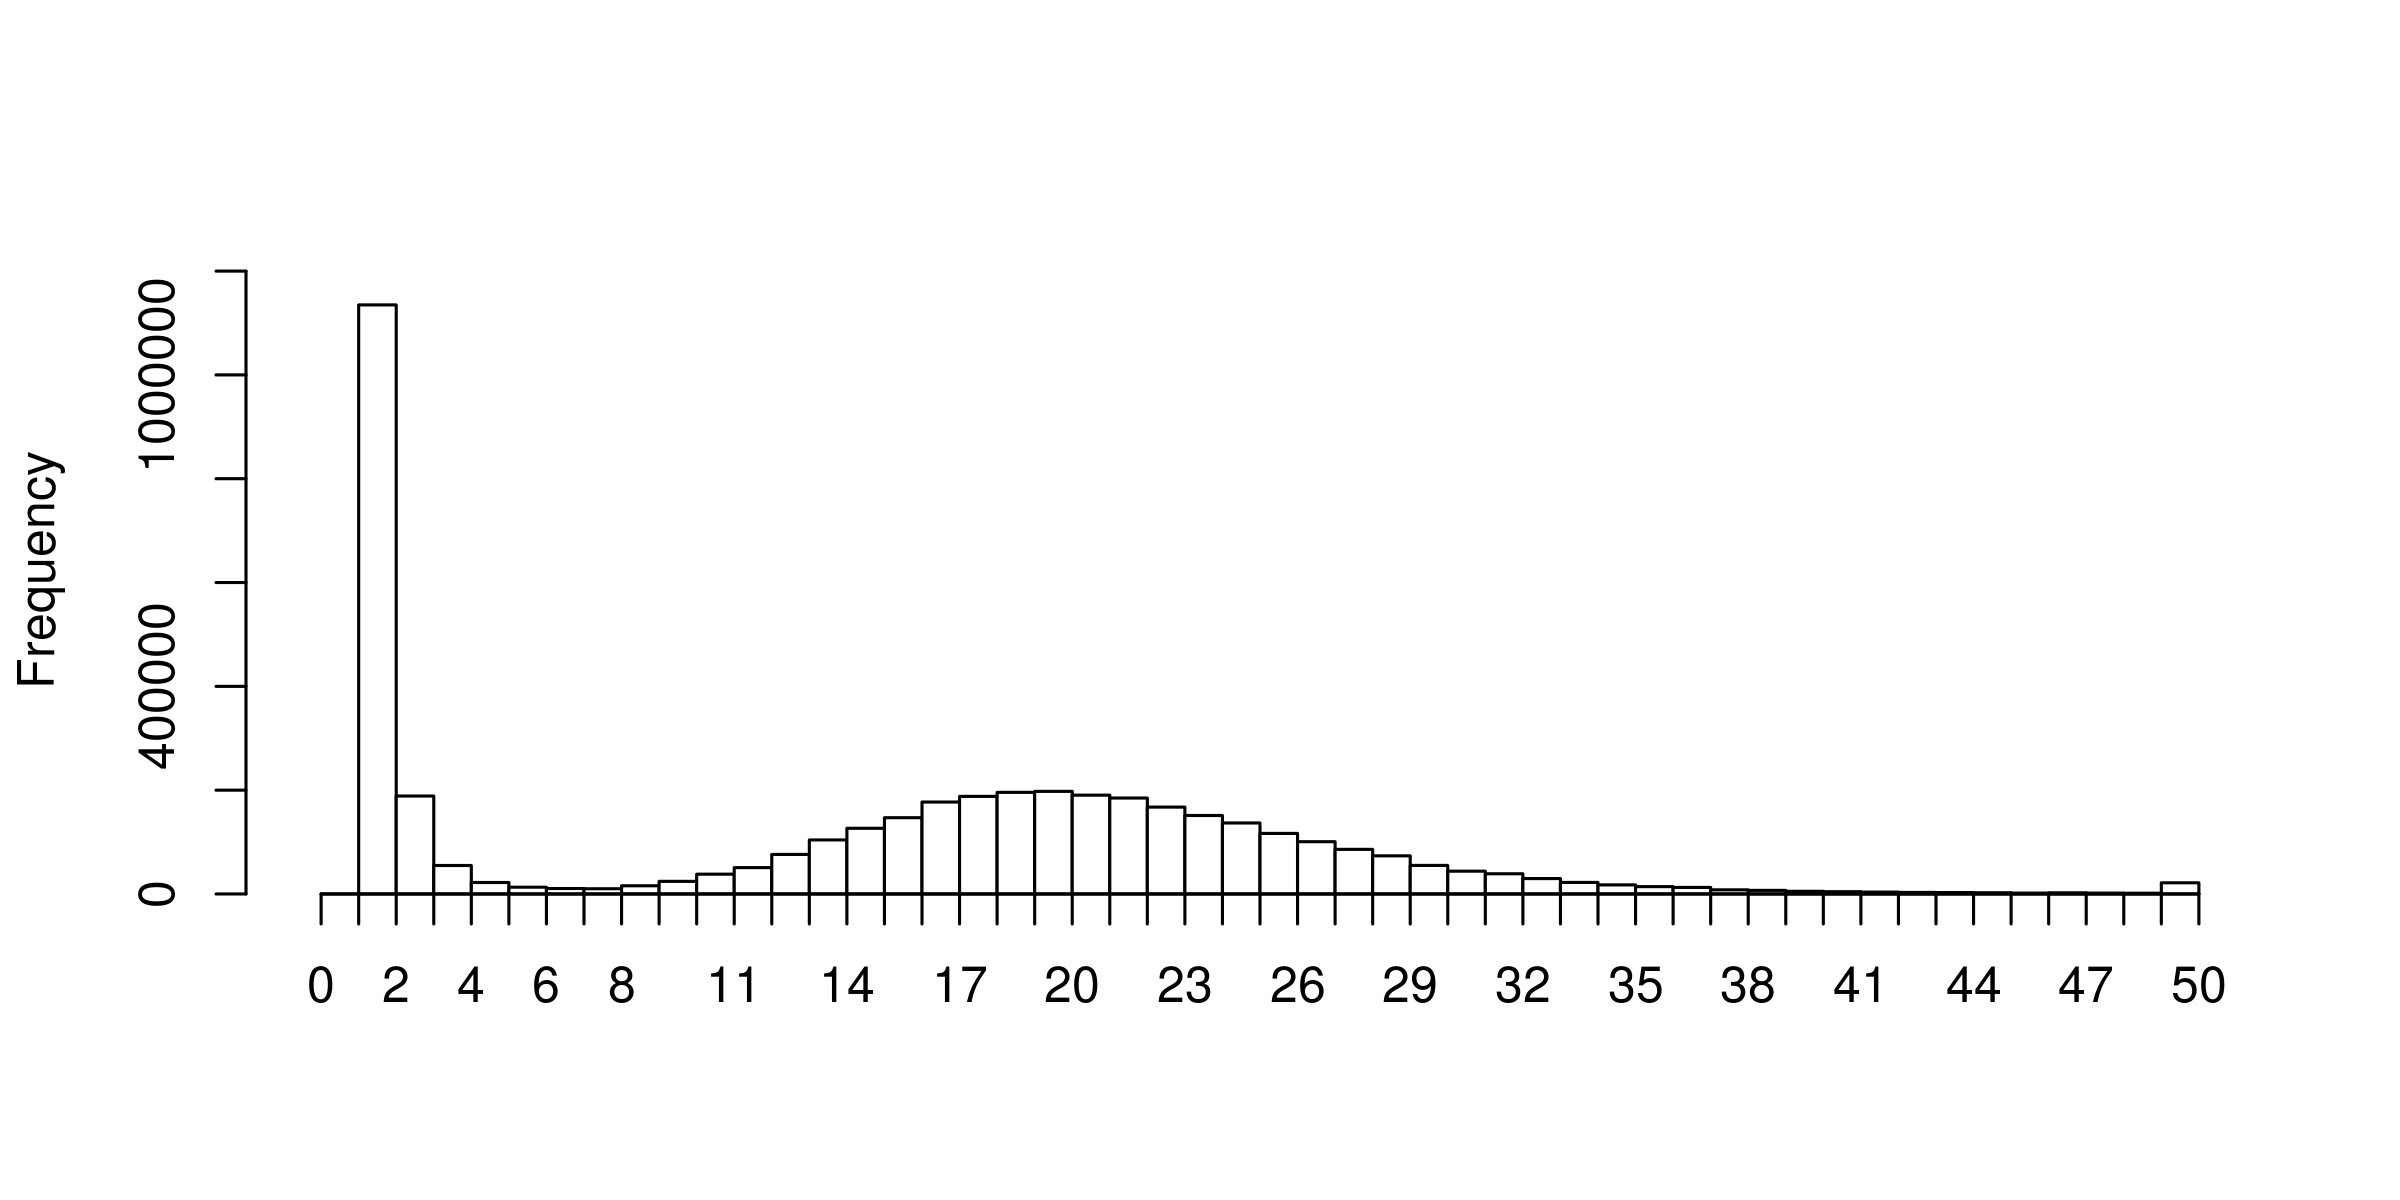
\includegraphics[width=0.8\textwidth]{de_novo/velvet/velvet_Rplot003.png}
\caption{\label{fig:velvetRplot003}}
\end{figure}

For me the histogram suggests to me to choose a coverage cut-off of around 9
with an expected coverage of about 19.

If you disagree, feel free to try different settings, but first leave R before
running \texttt{velvetg}:
\begin{lstlisting}[style=R]
q()
\end{lstlisting}

\begin{lstlisting}
cp run_25/contigs.fa run_25/contigs.fa.0

time velvetg run_25 -long_cov_cutoff 9
cp run_25/contigs.fa run_25/contigs.fa.1

time velvetg run_25 -long_cov_cutoff 9 -exp_cov 19
cp run_25/contigs.fa run_25/contigs.fa.2

gnx -min 100 -nx 25,50,75 run_25/contigs.fa*
\end{lstlisting}

\end{steps}

\begin{questions}
What is the N50 and runtime using:\\
\texttt{-long\_cov\_cutoff 9}
\begin{answer}
\texttt{5,747; real  0m11.457s; user  0m10.855s; sys  0m0.329s}
\end{answer}

\texttt{-long\_cov\_cutoff 9 -exp\_cov 19}
\begin{answer}
\texttt{16,781; real 0m29.830s; user 2m32.530s; sys 0m3.523s}
\end{answer}

other runs?

Which other parameters could improve the assembly quality for long reads?
\begin{answer}
\texttt{-conserveLong}
\end{answer}

What do you think about assembling 454 reads with Velvet?
\begin{answer}
It's working!
\end{answer}
\end{questions}


%\section{Assembling Multiple Insert Length Libraries}

\begin{note}
Like the previous examples, the data you will examine in this exercise is again
from Staphylococcus aureus which still has a genome of around 3MB. The reads are
Illumina paired end with an insert size of 170 bp and 350 bp.

You already downloaded the required reads from the SRA in previous exercises.
Specifically, the run data (SRR022863, SRR022852) from the SRA Study SRP001086.

\center{\url{http://www.ebi.ac.uk/ena/data/view/SRP001086}}
\end{note}

\begin{information}
The following exercise focuses on handing two insert length libraries with
velvet and the changes you have to look out for.
\end{information}

\begin{steps}
First move to the directory you made for this exercise, make a suitable named
directory for the exercise and check if all the files are in place:
\begin{lstlisting}
cd ~/NGS/velvet/part3
mkdir SRP001086
cd SRP001086
ln -s ~/NGS/Data/SRR022863_?.fastq.gz ./
ln -s ~/NGS/Data/SRR022852_?.fastq.gz ./
\end{lstlisting}

Now run \texttt{velveth} and \texttt{velvetg} using the appropriate command line
options by typing:
\begin{lstlisting}
time velveth run_25 25 -fmtAuto -create_binary -shortPaired -separate SRR022863_1.fastq.gz SRR022863_2.fastq.gz -shortPaired2 -separate SRR022852_1.fastq.gz SRR022852_2.fastq.gz
time velvetg run_25
\end{lstlisting}

The right thing to do is to run velvetg setting the cut-offs. To investigate
with R, as you did in the previous exercises, start up R and produce the
weighted histogram using the columns \texttt{short1\_cov} and
\texttt{short2\_cov} by typing:
\begin{lstlisting}[style=R]
R --no-save
library(plotrix) 
data <- read.table("run_25/stats.txt", header=TRUE) 
weighted.hist(data$short1_cov+data$short2_cov, data$lgth, breaks=0:70)
\end{lstlisting}

\begin{figure}[H]
\centering
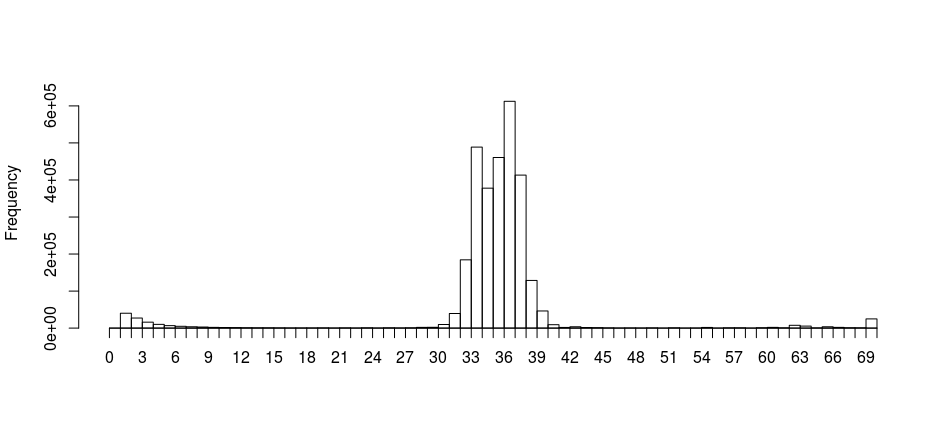
\includegraphics[width=0.8\textwidth]{de_novo/velvet/velvet_Rplot004.png}
\caption{\label{fig:velvet_Rplot004}}
\end{figure}

For me the histogram suggests a coverage cut-off of around 28
with an expected coverage of about 36. If you disagree, feel free to try
different settings, but first leave R before running \texttt{velvetg} with the coverage
parameters typing:
\begin{lstlisting}[style=R]
q()
\end{lstlisting}

\begin{lstlisting}
cp run_25/contigs.fa run_25/contigs.fa.0

time velvetg run_25 -cov_cutoff 28 
cp run_25/contigs.fa run_25/contigs.fa.1

time velvetg run_25 -cov_cutoff 28 -exp_cov 36 
cp run_25/contigs.fa run_25/contigs.fa.2

time velvetg run_25 -cov_cutoff 28 -exp_cov 36 -ins_length 170 -ins_length2 350
cp run_25/contigs.fa run_25/contigs.fa.3

gnx -min 100 -nx 25,50,75 run_25/contigs.fa*
\end{lstlisting}

\end{steps}

\begin{questions}
What was the best N50 you got?
\begin{answer}
62,741 bp
\end{answer}

How did the runtime/results compare to a run with a single paired-end library?
\begin{answer}
More memory, longer runtime, (in this case) similar results
\end{answer}

How many different libraries would you be able to run with this velvet version?
\begin{answer}
2 paired-end (or mate-pair) + one single end
\end{answer}

Would you be able to add a single-end library as well with this velvet version?
\begin{answer}
Yes
\end{answer}
\end{questions}


\begin{bonus}
Output an AMOS message file, convert it into an AMOS bank, update the
estimations for the insert size distributions and view the assembly with
Hawkeye.

\begin{lstlisting}
time velvetg run_25 -cov_cutoff 28 -exp_cov 36 -ins_length 170 -ins_length2 350 -amos_file yes -read_trkg yes
cp run_25/contigs.fa run_25/contigs.fa.4
gnx -min 100 -nx 25,50,75 run_25/contigs.fa.4

bank-transact -c -b run_25/velvet_asm.bnk -m run_25/velvet_asm.afg
asmQC -b run_25/velvet_asm.bnk -scaff -recompute -update -numsd 2
hawkeye run_25/velvet_asm.bnk
\end{lstlisting}

\begin{questions}
What are the mean and SD for the insert size distributions for the two libraries
used in the assembly?
\begin{answer}
Mean: 129; SD:31
Mean: 227; SD:19
\end{answer}
\end{questions}

\end{bonus}

% \begin{bonus}
% Find and download a different insert length library
% % TODO: \footnote affects the width of the shaded box - \renewcommand{\footnote}?
% \footnotemark[1]
% from the
% study SRP001086 and recompile velvet to allow the use of three insert length
% libraries. Maybe you could use the library you trimmed during previous
% exercises. You should be able to find these files here:
% \texttt{~/NGS/velvet/part2/SRX008042/SRR023408\_trim?.fastq}. If you don't still
% have these files, you can find a copy of them here:
% \texttt{~/NGS/Data/SRR023408\_trim?.fastq}.
% Use the fresh compiled Velvet version with the three (two provided and one
% downloaded library) to assemble the genome.
% \begin{questions}
% Does the extra library make any difference?
% \begin{answer}
% % TODO
% \end{answer}
% 
% How does the overall coverage change?
% \begin{answer}
% % TODO
% \end{answer}
% 
% Any other comments?
% \begin{answer}
% % TODO
% \end{answer}
% \end{questions}
% \footnotetext[1]{Paired insert
% lengths can be found on the NCBI SRA page in the library section (Nominal
% length) e.g. \url{http://www.ncbi.nlm.nih.gov/sra?term=SRR022866}}
% \end{bonus}


\begin{advanced}
\section{Hybrid Assembly}
\begin{note}
Like the previous examples, the data you will examine in this exercise is again
from Staphylococcus aureus which has a genome of around 3MB. The reads are 454
single end and Illumina paired end with an insert size of 170 bp.
You already downloaded the required reads from the SRA in previous exercises.
Specifically, the run data (SRR022863, SRR000892, SRR000893) from the SRA
experiments SRX007709 and SRX000181.
\end{note}

\begin{information}
The following exercise focuses on handing 454 long reads and paired-end reads
with velvet and the differences in setting parameters.
\end{information}

\begin{steps}
First move to the directory you made for this exercise, make a suitable named
directory for the exercise and check if all the three files are in place:
\begin{lstlisting}
cd ~/NGS/velvet/part3
mkdir SRR000892-SRR022863 
cd SRR000892-SRR022863
# 454 single end data
ln -s ~/NGS/Data/SRR00089[2-3].fastq.gz ./
# illumina paired end data
ln -s ~/NGS/Data/SRR022863_?.fastq.gz ./
\end{lstlisting}
\end{steps}

\begin{warning}
The following command will run for a LONG time. This indicated the amount of
calculations being preformed by Velvet to reach a conclusion. To wait for velvet
to finish would exceed the time available in this workshop, but it is up to you
to either let it run over night or kill the process by using the key combination
\texttt{CTRL+c}.
\begin{lstlisting}
velveth run_25 25 -fmtAuto -create_binary -long SRR00089?.fastq.gz -shortPaired -separate SRR022863_1.fastq.gz SRR022863_2.fastq.gz
time velvetg run_25
\end{lstlisting}

\begin{steps}
If you have decided to continue, we already inspected the weighted histograms
for the short and long read library separately, you can reuse this for the
cut-off values:
\begin{lstlisting}
time velvetg run_25 -cov_cutoff 7 -long_cov_cutoff 9
\end{lstlisting}
\end{steps}

\begin{questions}
What are your conclusions using Velvet in an hybrid assembly?
\begin{answer}
17 min:  time velvetg run\_25
\end{answer}
\end{questions}

\end{warning}
\end{advanced}



%
% End of modules
% Switch back to normal workshop chapter styling
%
\chapterstyle{workshop}



\chapter{Post-Workshop Information}
\clearpage
%
% Access to Computational Resources
%
\section{Access to Computational Resources}

By the end of the workshop we hope you're thinking one or more of the following:

\begin{itemize}
\item I'm interested in dabbling some more during my day-job!
\item How do I access a Linux box like the one I've been using in the workshop -
I \emph{really} don't want the hassle of setting this all up myself!
\item I'm hooked! I \emph{really} want to get down and dirty with NGS data! What
computational resources do I need, what do I have access to and how do I access
them?
\end{itemize}

We're ecstatic you're thinking this way and want to help guide you! However, lets
take this one step at a time.

The quickest way to dabble is to use a clone of the operating system (OS) you've
been using during this workshop. That means you'll have hassle-free access to a
plethora of pre-installed, pre-configured bioinformatics tools. You could even set it
up to contain a copy of all the workshop data and handouts etc to go through the
hands-on practicals in your own time!

We have created an image file (approx. 10 GBytes in size) of the NGS Training OS for you to
use as you wish:
\\\\
%\url{https://swift.rc.nectar.org.au:8888/v1/AUTH_809/NGSImage/NGSTrainingV1.0.vdi}
\url{https://swift.rc.nectar.org.au:8888/v1/AUTH_33065ff5c34a4652aa2fefb292b3195a/VMs/NGSTrainingV1.2.1.vdi}
\\\\
We would advise one of the following two approaches for making use of it:

\begin{itemize}
\item Import it into VirtualBox to setup a virtual machine (VM) on your own
computer.
\item Instantiate a VM on the NeCTAR Research Cloud.
\end{itemize}

\subsection{Setting up a VM using VirtualBox}
This approach requires the least amount of mind-bending to get up and running.
However, you will need to install some software. If you do not have
administrator access or your system administrator is slow or unwilling to
install the software, you may find using the NeCTAR Research Cloud to be viable
alternative.

This approach will use, at most, the computational resources available on
your own computer. If you are analysing non-microbial organisms or performing
\textit{de novo} assemblies, you may find these resources are insufficient. If this is the
case, you really should speak to someone from IT support at your institution or
get in touch with a bioinformatician for advise.

The software you need is VirtualBox, a freely available, Open Source
virtualisation product from Oracle (\url{https://www.virtualbox.org/}). This
software essentially allows you to run an operating system (the guest OS) within
another (the host OS). VirtualBox is available for several different host OSes
including MS Windows, OS X, Linux and Solaris
(\url{https://www.virtualbox.org/wiki/Downloads}). Once VirtualBox is installed
on your host OS, you can then install a guest OS inside VirtualBox. VirtualBox
supports a lot of different OSes
(\url{https://www.virtualbox.org/wiki/Guest_OSes}).

Here are the steps to setting up a VM in VirtualBox with our image file:
\begin{enumerate}
  \item Download and install VirtualBox for your OS: 
  \url{https://www.virtualbox.org/wiki/Downloads}
  \item Start VirtualBox and click New to start the Create New Virtual Machine wizard
  \item Give the VM a useful name like ``NGS Training'' and choose Linux and
  either Ubuntu or Ubuntu (64-bit) as the OS Type
  \item Give the VM access to a reasonable amount of the host Oses memory. i.e.
  somewhere near the top of the green. If this value is $<$ 2000 MB, you are
  likely to have insufficient memory for your NGS data analysis needs.
  \item For the virtual hard disk, select ``Use existing hard disk'' and browse
  to and select the \texttt{NGSTrainingV1.2.1.vdi} file you downloaded.
  \item Confirm remaining settings
  \item Select the ``NGS Training'' VM and click Start to boot he machine.
  \item Once booted, log into the VM as either \texttt{ubuntu} (a sudoer user;
  i.e. has admin rights) or as \texttt{ngstrainee} (a regular unprivileged
  user). See table below for passwords.
\end{enumerate}


\subsection{Setting up a VM using the NeCTAR Research Cloud}
All Australian researchers, who are members of an institution which subscribes
to the Australian Access Federation (AAF; \url{http://www.aaf.edu.au/}), have
access to a small amount of computing resources (2 CPU's and 8 GBytes RAM) on
the NeCTAR Research Cloud (\url{http://nectar.org.au/research-cloud}).

\subsubsection{Login to the NeCTAR Research Cloud Dashboard}
The online dashboard is a graphical interface for administering (creating,
deleting, rebooting etc) your virtual machines (VMs) on the NeCTAR research
cloud.

\begin{enumerate}
  \item Go to the dashboard: \url{http://dashboard.rc.nectar.org.au}
  \item When you see the following page, click the ``Log In" button:
  \begin{figure}[H]
    \centering
    
\includegraphics[scale=0.5]{post-workshop/nectar/aaf_login.png}
    \caption{\label{fig:aaf_login}}
  \end{figure}
  \item At the following screen, simply choose your institution from the
  dropdown box and click ``Select". Now follow the on screen prompts and enter
  your regular institutional login details.
  \begin{figure}[H]
    \centering
    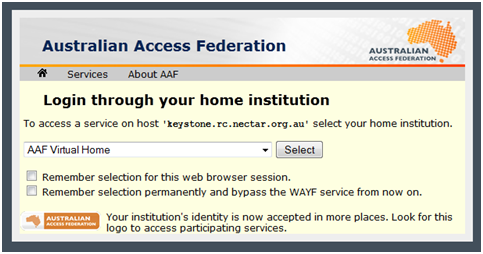
\includegraphics[scale=0.5]{post-workshop/nectar/aaf_home_institute.png}
    \caption{\label{fig:aaf_home_institute}}
  \end{figure}
  \item If you see the following screen, congratulations, you have
  successfully logged into the NeCTAR Research Cloud dashboard!
  \begin{figure}[H]
    \centering
    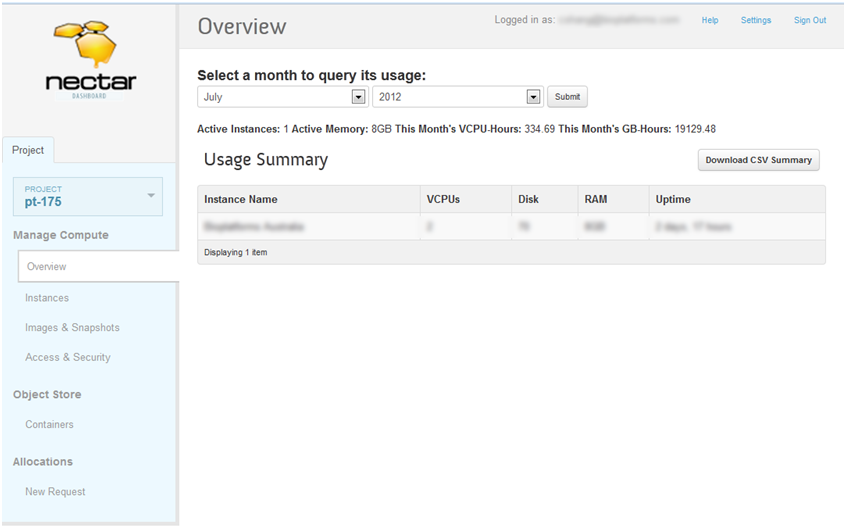
\includegraphics[scale=0.5]{post-workshop/nectar/dashboard_overview.png}
    \caption{\label{fig:dashboard_overview}}
  \end{figure}
\end{enumerate}

\subsubsection{Instantiating Your Own VM}
We will now show you how to instantiate the ``NGS Training'' image using your
own personal cloud allocation.

\begin{enumerate}
  \item In the NeCTAR Research Cloud dashboard, click ``Images \& Snapshots''
  to list all the publicly available images from which you can instantiate a
  VM. Under ``Snapshots" Click the ``Launch" button for the latest version of the
  ``NGSTraining" snapshot:
  \begin{figure}[H]
    \centering
    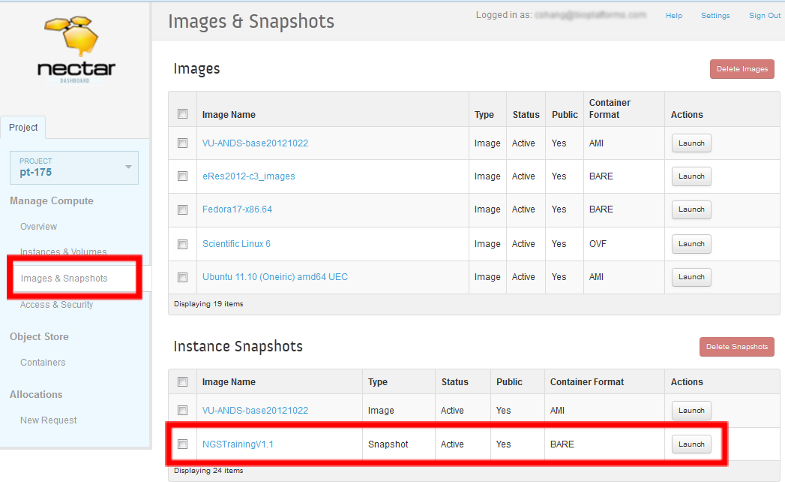
\includegraphics[scale=0.5]{post-workshop/nectar/dashboard_snapshots.png}
    \caption{\label{fig:dashboard_snapshots}}
  \end{figure}
  \item You will now see a ``Launch Instances'' window where you are required to
  enter some details about how you want the VM to be setup before clicking
  ``Launch Instance".
  In the ``Launch Instances'' pop-up frame choose the following settings:
  \begin{description}
  \item[Server Name] A human readable name for your convenience. e.g. ``My NGS VM''
  \item[Flavor] The resources you want to allocate to this VM. I suggest a
  Medium sized VM (2 CPUs and 8 GBytes RAM). This will use all your personal
  allocation, but anything less will probably be insufficient. You could request
  a new allocation of resources if you want to instantiate a larger VM with more
  memory.
  \item[Security Groups] Select SSH.
  \end{description}
  \item Click the ``Launch Instance'' button
  \begin{figure}[H]
    \centering
    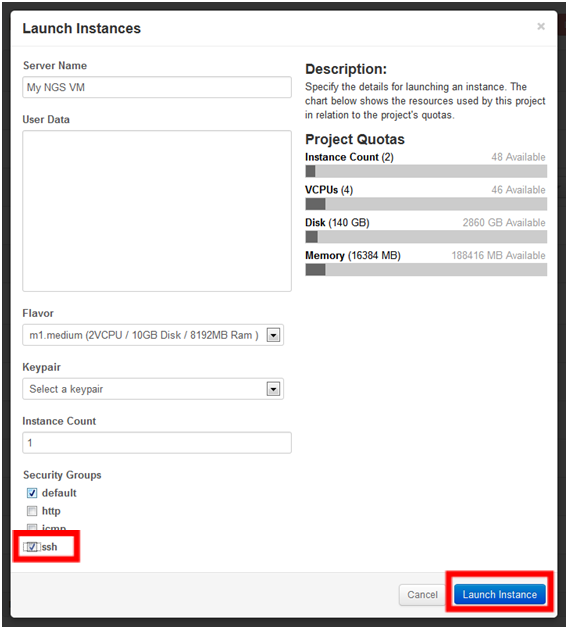
\includegraphics[scale=0.5]{post-workshop/nectar/dashboard_launch.png}
    \caption{\label{fig:dashboard_launch}}
  \end{figure}
  \item You will be taken to the ``Instances" page and you will see the
  ``Status" and ``Task" column for your new VM is ``Building" and ``Spawning". Once
  the ``IP Address" cell is populated, take a note of it as you will need it for
  configuring the NX Client later on.
  \begin{figure}[H]
    \centering
    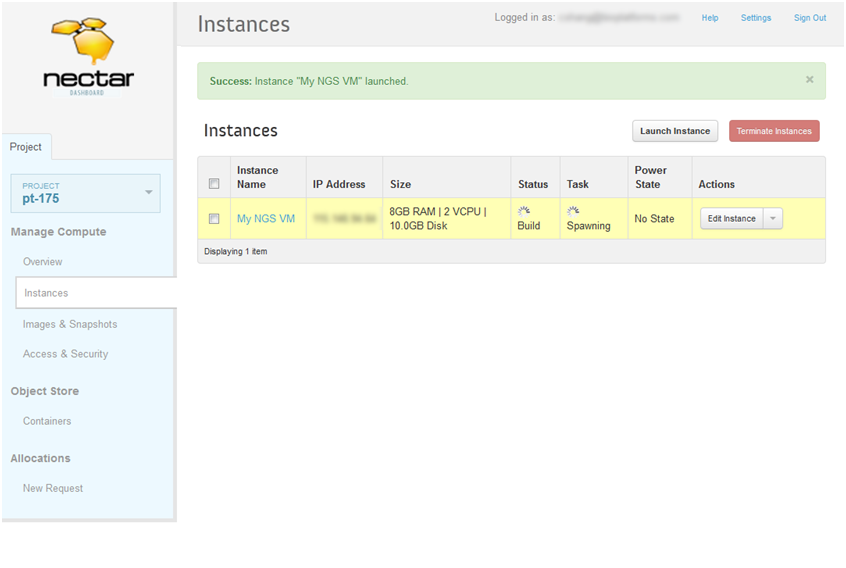
\includegraphics[scale=0.5]{post-workshop/nectar/dashboard_instance_building.png}
    \caption{\label{fig:dashboard_instance_building}}
  \end{figure}
  \item Once the Status and Task for the VM change to ``Active and ``None"
  respectively, your VM is powered up and is configuring itself.
  Congratulations, you have now instantiated a Virtual Machine! If you try to
  connect to the VM too quickly, you might not be successful. The OS may still
  be configuring itself, so give it a few minutes to finish before continuing.
  \begin{figure}[H]
    \centering
    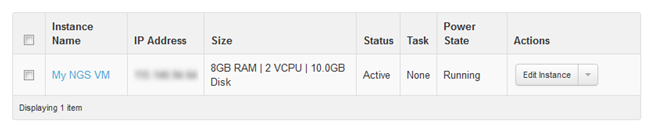
\includegraphics[scale=0.5]{post-workshop/nectar/dashboard_instance_running.png}
    \caption{\label{fig:dashboard_instance_running}}
  \end{figure}
\end{enumerate}

\subsubsection{VM Stuck Building and Spawning}
Sometimes, the cloud experiences a ``hiccup" and a newly instantiated VM will get
stuck in the ``Build" and ``Spawning" state (step 3) for more than a few minutes.
This can be rectified by terminating the instance and creating a new VM from
scratch:
\begin{enumerate}
  \item Selecting ``Terminate Instance" under the ``Edit Instance" dropdown box:
  \begin{figure}[H]
    \centering
    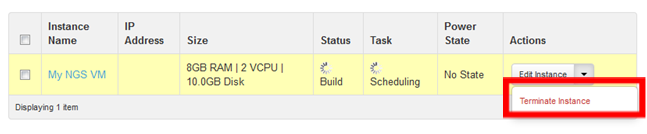
\includegraphics[scale=0.5]{post-workshop/nectar/dashboard_terminate_stuck_instance.png}
    \caption{\label{fig:dashboard_terminate_stuck_instance}}
  \end{figure}
  \item Go back to step 1 of ``Instantiating Your Own VM" and create the VM from scratch:
\end{enumerate}
  

\subsection{Remote Desktop with the NoMachine NX Client}
During the workshop you were using the free NX client from NoMachine
(\url{http://www.nomachine.com/}) to provide a remote desktop-like connection to
VMs running on the NeCTAR Research Cloud. Therefore, we provide information on how to
setup your local computer to connect to the VM you just instantiated in the steps
above.

We assume that:
\begin{itemize}
\item You have administrator rights on your local computer for installing
software.
\end{itemize}

\subsubsection{NoMachine NX Client Installing}
We show you instructions below for the MS Windows version of the NX Client, but
procedures for other supported OSes (Linux, Mac OSX and Solaris) should be very
similar.
\begin{enumerate}
  \item Go to the NoMachine download page: \url{http://www.nomachine.com/download.php}
  \item Click the download icon next to the NX Client for Windows:
  \begin{figure}[H]
    \centering
    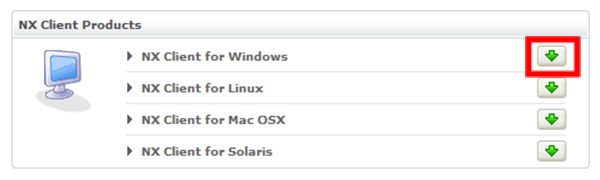
\includegraphics[scale=0.5]{post-workshop/nx_client/download.png}
    \caption{\label{fig:nx_download}}
  \end{figure}
  \item On the "NX Client for Windows" page, click the "Download package" button:
  \begin{figure}[H]
    \centering
    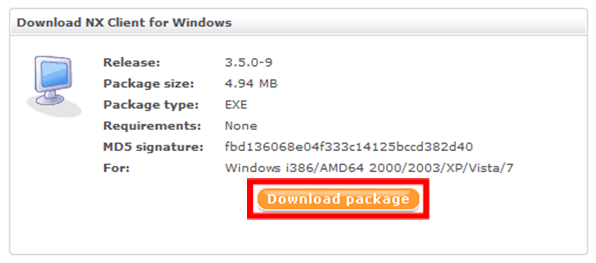
\includegraphics[scale=0.5]{post-workshop/nx_client/download_package.png}
    \caption{\label{fig:nx_download_package}}
  \end{figure}
  \item Run the file you just downloaded (accepting defaults is fine)
  \item Congratulations, you just installed the NoMachine NX Client!
\end{enumerate}

\subsection{NoMachine NX Client Configuration}
Now we have the NoMachine NX Client installed, we need to configure a new NX
"session" which will point to the VM we instantiated in the NeCTAR Research
Cloud.

We assume that:
\begin{itemize}
\item You know the IP address of the VM you want to remote desktop into.
\end{itemize}

\begin{enumerate}
  \item Start the NX Connection Wizard and click "Next" to advance to the
  "Session" settings page.
  \begin{figure}[H]
    \centering
    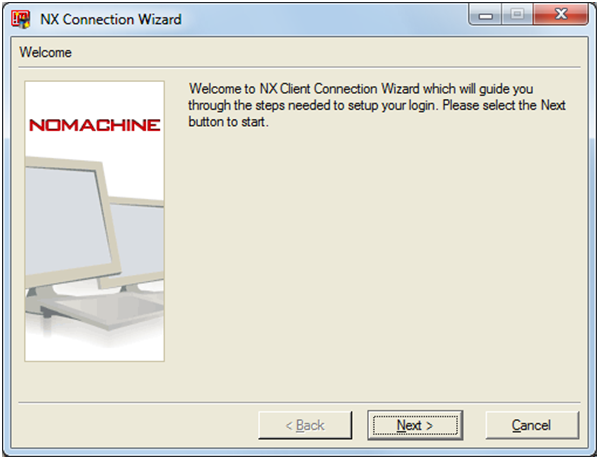
\includegraphics[scale=0.5]{post-workshop/nx_client/start_wizard.png}
    \caption{\label{fig:nx_start_wizard}}
  \end{figure}
  \item On the "Sessions" settings page enter the following details:
  \begin{description}
  \item[Session] A memorable name so you know which VM this session is pointing
  at. You could use the same name you chose for the VM you instantiated earlier
  e.g. "NGS Training".
  \item[Host] Enter the IP address of the VM you instantiated on the NeCTAR
  Research Cloud.
  \begin{figure}[H]
    \centering
    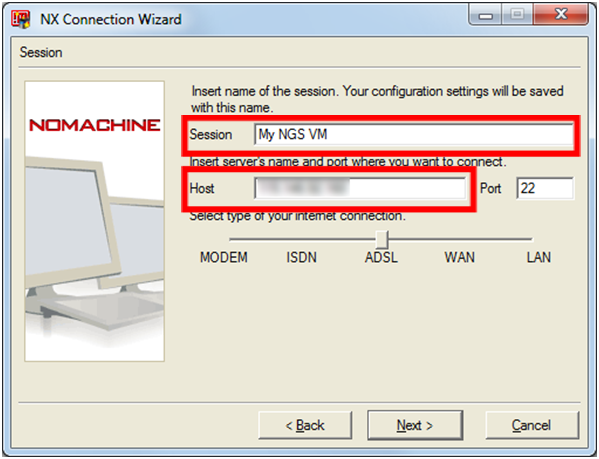
\includegraphics[scale=0.5]{post-workshop/nx_client/session_configuration.png}
    \caption{\label{fig:nx_session_configuration}}
  \end{figure}
  \end{description}
  \item Click "Next" to advance to the "Desktop" settings page. You should use the
  "Unix GNOME" setting.
  \begin{figure}[H]
    \centering
    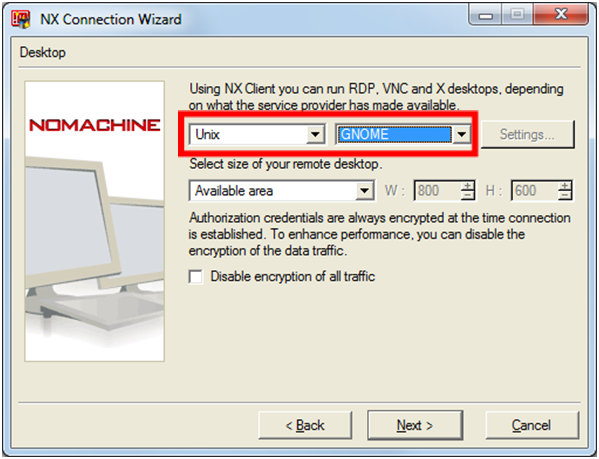
\includegraphics[scale=0.5]{post-workshop/nx_client/desktop_type.png}
    \caption{\label{fig:nx_desktop_type}}
  \end{figure}
  \item Click "Next" and "Finish" to complete the wizard.
\end{enumerate}

\subsection{Connecting to a VM}
If you just completed the NX Connection Wizard described above, the wizard
should have opened the NX Client window. If not, run the "NX Client". You will
be presented with a window like this:
\begin{figure}[H]
  \centering
  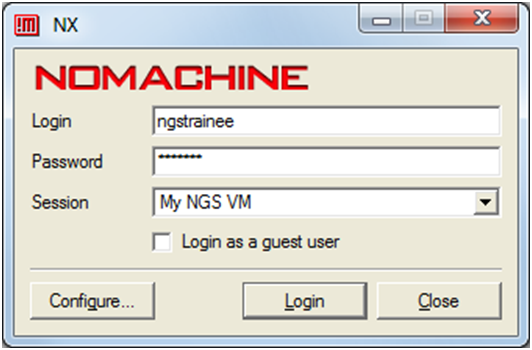
\includegraphics[scale=0.5]{post-workshop/nx_client/login.png}
  \caption{\label{fig:nx_login}}
\end{figure}

The "Login" and "Password" boxes in the NX Client are for user accounts setup on
the VM. By default our image, from which you instantiated your VM, has two
preconfigured users:
\begin{figure}[H]
  \centering
  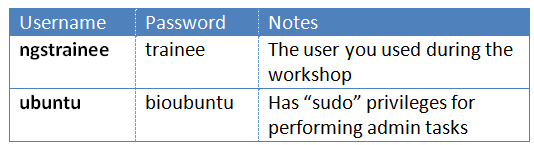
\includegraphics[scale=0.5]{post-workshop/nx_client/usernames_passwords.png}
  \caption{\label{fig:nx_usernames_passwords}}
\end{figure}

Unless you know what you are doing, we suggest you use the \texttt{ngstrainee}
user account details to initiate an NX connection to your VM. In less than a
minute, you should see an NX Window showing the desktop of your VM:
\begin{figure}[H]
  \centering
  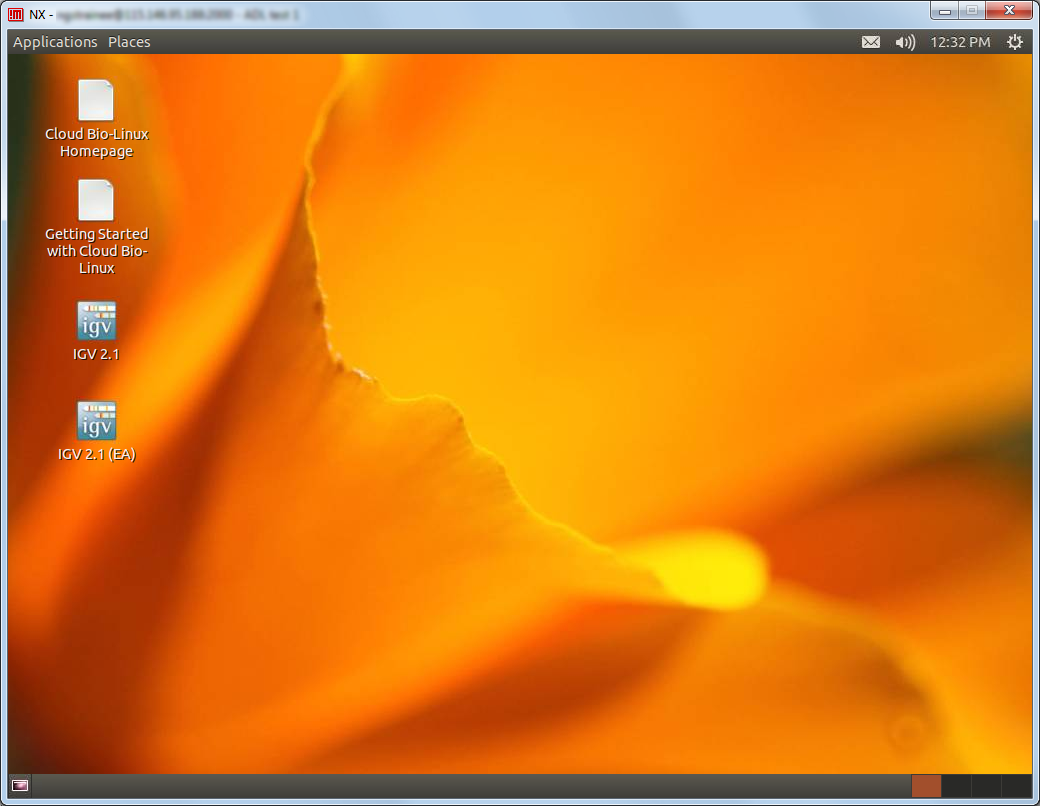
\includegraphics[width=0.8\textwidth]{post-workshop/nx_client/connected.png}
  \caption{\label{fig:nx_connected}}
\end{figure}

\subsection{NX Connection Failure}
In the event that you don't get the NX Window with your VM's desktop displaying
inside it. The most common errors are:
\begin{itemize}
\item You failed to select the "ssh" security group when instantiating the VM.
You'll need to terminate the instance and create a new VM from scratch
\item You failed to select "Unix GNOME" when you configured the NX Client
session. You'll need to reconfigure the session using the NX Client
\item Your institutions firewall blocks TCP port 22. You may need to request this
port to be opened by your local network team or configure the NX client to use a
proxy server.
\end{itemize}

\subsection{Advanced Configuration}
In the session configuration, you can configure the size of the NX Window in
which the desktop of the VM is drawn:
\begin{figure}[H]
  \centering
  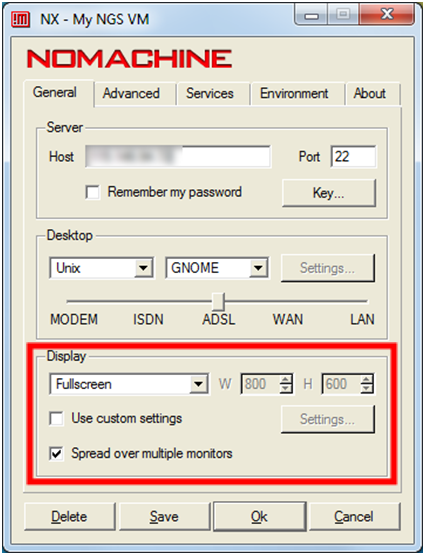
\includegraphics[scale=0.5]{post-workshop/nx_client/advanced_display.png}
  \caption{\label{fig:nx_advanced_display}}
\end{figure}

This can be useful if you want to:
\begin{itemize}
\item Have the NX Window occupy the entire screen, without window decorations.
This is often desirable if you wish to "hide" the host OS from the person
sitting at the computer running the NX Client.
\item Have the NX Window spread over multiple monitors.
\end{itemize}


\clearpage

%
% Access to Workshop Documents
%
\section{Access to Workshop Documents}

This document has been written in \LaTeX\ and deposited in a public github
repository (\url{https://github.com/nathanhaigh/ngs_workshop}). The
documentation has been released under a Creative Commons Attribution 3.0
Unported License (see the Licence page at the beginning of this handout).

For convienience, you can access up-to-date PDF versions of the \LaTeX\ documents at:
\begin{description}[style=multiline,labelindent=0cm,align=left,leftmargin=0.5cm]
\item[Trainee Handout]\hfill\\
\url{https://github.com/nathanhaigh/ngs_workshop/raw/master/trainee_handout.pdf}
\item[Trainer Handout]\hfill\\
\url{https://github.com/nathanhaigh/ngs_workshop/raw/master/trainer_handout.pdf}
\end{description}

\section{Access to Workshop Data}
Once you have created a VM from our image file, either locally using VirtualBox
or on the NeCTAR Research Cloud, you can configure the system with the workshop
documents and data. This way you can revisit and work through this workshop in
your own time.

In order to do this, we have provided you with access to a shell script which
should be executed on your NGS Training VM by the \texttt{ubuntu} user. This pulls
approx. 3.3 GBytes of data from the NeCTAR Cloud storage and configures the system
for running this workshop:

% NOTE This bash script could be entered into the user data when instantiating
% the VM in the first place
\begin{lstlisting}
# As the ubuntu user run the following commands:
cd /tmp
wget https://github.com/nathanhaigh/ngs_workshop/raw/master/\
workshop_deployment/NGS_workshop_deployment.sh
bash NGS_workshop_deployment.sh
\end{lstlisting}

While you're at it, you may also like to change the timezone of your VM to match
that of your own. To do this simply run the following commands as the
\texttt{ubuntu} user:
\begin{lstlisting}
TZ="Australia/Adelaide"
echo "$TZ" | sudo tee /etc/timezone
sudo dpkg-reconfigure --frontend noninteractive tzdata
\end{lstlisting}

For further information about what this script does and possible command line
arguments, see the script's help:
\begin{lstlisting}
bash NGS_workshop_deployment.sh -h
\end{lstlisting}


For further information about setting up the VM for the workshop, please see:
\\\\
\url{https://github.com/nathanhaigh/ngs_workshop/blob/master/workshop_deployment/README.md}


\chapter{Space for Personal Notes or Feedback}
\clearpage

%
% Some empty ruled comments pages
%
\myruledpage{3cm}{1cm}
\myruledpage{3cm}{1cm}
\myruledpage{3cm}{1cm}
\myruledpage{3cm}{1cm}

\end{document}
